\documentclass[Main.tex]{subfiles}
\begin{document}
%%%Phần mở đầu
%\chapter{Hợp chất của hiđro với halogen}
%\tatloigiai
\setcounter{section}{1}
\section{Hydrogen halide và axit halohidric}
\begin{Muctieu}
	\begin{itemize}
		\item Trình bày được thành phần phân tử, cấu tạo của các phân tử hydrogen halide (HX).
		\item Nêu được sự biến đổi nhiệt độ sôi của các hydrogen halide từ HF đến HI và giải thích được sự biến đổi này.
		\item Trình bày được tính chất vật lí, tính chất hoá học cơ bản của hydrohalic acid (tính acid, tính khử).
		\item Nêu được ứng dụng của một số hydrogen halide và hydrohalic acid trong đời sống và sản xuất.
		\item Giải thích được tính chất ăn mòn thuỷ tinh đặc biệt của hydrofluoric acid (HF).
	\end{itemize}
\end{Muctieu}
\begin{kd}
	\immini{Trong dạ dày của chúng ta có chứa một loại axit giúp tiêu hóa thức ăn, đó là axit clohidric ($HCl$). Ngoài ra, người ta còn dùng một loại axit khác để khắc các hoa văn tinh xảo lên thủy tinh. Các em có biết đó là axit gì không? $HCl$ và axit dùng khắc thủy tinh có những điểm gì chung và riêng về thành phần cấu tạo và tính chất? Chúng ta hãy cùng tìm hiểu trong bài học này nhé!}{}
\end{kd}

%%%Phần lý thuyết
\subsection{Nội dung bài học} 

\subsubsection{Hydrogen halide (HX)}
	\Noibat[\maunhan][][][]{Khái niệm và cấu tạo phân tử}
	\begin{ghinho}
		Hydrogen halide là hợp chất vô cơ có công thức chung là $HX$, trong đó $H$ là hydrogen và $X$ là một nguyên tố halogen (F, Cl, Br, I).
		Trong phân tử $HX$, nguyên tử $H$ và nguyên tử $X$ liên kết với nhau bằng một liên kết cộng hoá trị phân cực về phía nguyên tử halogen do halogen có độ âm điện lớn hơn hydrogen.
	\end{ghinho}

	\begin{hoivadap} 
        Dựa vào độ âm điện của các halogen (F=3.98, Cl=3.16, Br=2.96, I=2.66) và hydrogen (H=2.20), hãy so sánh độ phân cực của liên kết trong các phân tử $HF, HCl, HBr, HI$. Sự khác biệt về độ phân cực này ảnh hưởng như thế nào đến tính chất của chúng?
	\end{hoivadap}
	\Noibat[\maunhan][][][]{Tính chất vật lí}
	\begin{ghinho}
		Ở điều kiện thường, các hydrogen halide (HF, HCl, HBr, HI) đều là chất khí, không màu, mùi xốc, độc. Chúng dễ tan trong nước tạo thành các dung dịch hydrohalic acid tương ứng.
	\end{ghinho}
    \begin{Bancobiet}
        Khí $HCl$ khi tiếp xúc với không khí ẩm tạo thành các hạt nhỏ dung dịch $HCl$, giống như màn sương mù. Hiện tượng này được gọi là hiện tượng "bốc khói" của dung dịch $HCl$ đặc.
    \end{Bancobiet}
	\begin{tomtat}
		\textbf{Nhiệt độ sôi:} Nhiệt độ sôi của các hydrogen halide tăng dần từ $HCl$ đến $HI$ ($HCl < HBr < HI$). Riêng $HF$ có nhiệt độ sôi cao bất thường (19.5 $^\circ$C) so với các $HX$ còn lại.
	\end{tomtat}

    \begin{center}
		\textbf{Bảng: Nhiệt độ sôi của các hydrogen halide}\\
        \begin{tabular}{|c|c|c|c|c|}
            \hline
            \textbf{Chất} & \textbf{HF} & \textbf{HCl} & \textbf{HBr} & \textbf{HI} \\ 
            \hline
            Nhiệt độ sôi ($^\circ$C) & 19.5 & -85.1 & -66.8 & -35.4 \\
            \hline
        \end{tabular}
		\captionof{table}{Nhiệt độ sôi của một số hydrogen halide}
    \end{center}
	\begin{hoivadap}
		Tại sao $HF$ lại có nhiệt độ sôi cao bất thường so với $HCl$, $HBr$, $HI$? Yếu tố nào quyết định sự tăng dần nhiệt độ sôi từ $HCl$ đến $HI$? (Gợi ý: Liên kết hydrogen, khối lượng phân tử).
	\end{hoivadap}
	\begin{ghinho}
		Nguyên nhân $HF$ có nhiệt độ sôi cao bất thường là do giữa các phân tử $HF$ còn có liên kết yếu đặc biệt là \textbf{liên kết hydrogen} ($F^{\delta-}$---$H^{\delta+}$). Liên kết hydrogen trong $HF$ bền hơn nhiều so với liên kết hydrogen trong nước.
        Sự tăng nhiệt độ sôi từ $HCl$ đến $HI$ là do sự tăng khối lượng phân tử làm tăng lực tương tác van der Waals giữa các phân tử.
	\end{ghinho}

\subsubsection{Hydrohalic acid (Dung dịch HX)}
	\Noibat[\maunhan][][][]{Tính acid}
	\begin{ghinho}
		Khi tan trong nước, các hydrogen halide ($HX$) phân li ra ion $H^+$, thể hiện tính acid. Tên gọi của dung dịch axit: Hydrofluoric acid (HF), Hydrochloric acid (HCl), Hydrobromic acid (HBr), Hydroiodic acid (HI).
		Phương trình điện li tổng quát: $HX \rightleftharpoons H^+ + X^-$
	\end{ghinho}
	\begin{tomtat}
		Tính acid của các dung dịch hydrohalic acid tăng dần theo dãy: $HF < HCl < HBr < HI$.
        Trong đó, $HF$ là acid yếu, còn $HCl, HBr, HI$ là các acid mạnh.
	\end{tomtat}
	\begin{hoivadap}
		Tại sao tính acid lại tăng dần từ $HF$ đến $HI$ trong khi độ phân cực của liên kết lại giảm dần? Yếu tố nào quyết định độ mạnh yếu của acid trong dãy này? (Gợi ý: Năng lượng liên kết H-X)
	\end{hoivadap}
    \begin{ghinho}
        Độ mạnh của acid trong dãy $HX$ phụ thuộc chủ yếu vào độ bền liên kết $H-X$. Liên kết $H-F$ bền nhất nên $HF$ khó phân li ra $H^+$ nhất (acid yếu). Liên kết $H-I$ kém bền nhất nên $HI$ dễ phân li ra $H^+$ nhất (acid mạnh nhất).
    \end{ghinho}
    \begin{hopdongian}
        \textbf{Tính chất chung của acid:}
        \begin{itemize}
            \item Làm đổi màu chất chỉ thị (quỳ tím hóa đỏ).
            \item Tác dụng với kim loại đứng trước H trong dãy hoạt động hóa học $\rightarrow$ muối + $H_2$. Ví dụ: $Fe + 2HCl \rightarrow FeCl_2 + H_2$
            \item Tác dụng với basic oxide $\rightarrow$ muối + $H_2O$. Ví dụ: $CuO + 2HCl \rightarrow CuCl_2 + H_2O$
            \item Tác dụng với base $\rightarrow$ muối + $H_2O$. Ví dụ: $HBr + NaOH \rightarrow NaBr + H_2O$
            \item Tác dụng với muối của acid yếu hơn $\rightarrow$ muối mới + acid mới yếu hơn. Ví dụ: $2HCl + CaCO_3 \rightarrow CaCl_2 + H_2O + CO_2$
        \end{itemize}
    \end{hopdongian}
	\Noibat[\maunhan][][][]{Tính khử}
	\begin{ghinho}
		Trong các hợp chất $HX$, các halogen $X$ có số oxi hóa thấp nhất là -1. Do đó, ion halide $X^-$ có khả năng nhường electron, thể hiện tính khử.\\
		Ví dụ: $MnO_2 + 4HCl \xrightarrow[$t^\circ$] MnCl_2 + Cl_2 + 2H_2O$ (Trong phản ứng này, $Cl^-$ đã nhường electron để thành $Cl_2$, thể hiện tính khử).
	\end{ghinho}
	\begin{tomtat}
		Tính khử của các ion halide tăng dần theo dãy: $F^- < Cl^- < Br^- < I^-$.
		$F^-$ hầu như không thể hiện tính khử trong dung dịch.
		$Cl^-$ thể hiện tính khử khi tác dụng với chất oxi hóa mạnh ($MnO_2, KMnO_4, K_2Cr_2O_7$,...).
		$Br^-$ và $I^-$ có tính khử mạnh hơn $Cl^-$, có thể bị oxi hóa bởi các chất oxi hóa yếu hơn (như $Cl_2$, $H_2SO_4$ đặc).
	\end{tomtat}
	\begin{hoivadap}
        Tại sao tính khử lại tăng dần từ $F^-$ đến $I^-$? Yếu tố nào ảnh hưởng đến khả năng nhường electron của ion $X^-$? (Gợi ý: Bán kính ion, độ âm điện).
	\end{hoivadap}
     \begin{ghinho}
         Tính khử tăng từ $F^-$ đến $I^-$ là do bán kính ion tăng dần, làm cho lớp electron ngoài cùng xa hạt nhân hơn, dễ bị tách ra hơn (khả năng nhường electron tăng).
     \end{ghinho}
	\Noibat[\maunhan][][][]{Tính chất đặc biệt của Hydrofluoric acid (HF)}
	\begin{ghinho}
		Hydrofluoric acid ($HF$) có khả năng ăn mòn các đồ vật làm bằng thủy tinh (thành phần chính là silicon dioxide, $SiO_2$). Do đó, $HF$ được dùng để khắc chữ, họa tiết trên thủy tinh.
		Phương trình phản ứng: $SiO_2 + 4HF \rightarrow SiF_4\uparrow (\text{silicon tetrafluoride}) + 2H_2O$
	\end{ghinho}
	\begin{Bancobiet}
		Vì HF ăn mòn thủy tinh nên không thể đựng dung dịch HF trong các chai lọ thủy tinh thông thường mà phải đựng trong các bình chứa bằng nhựa (polyethylene) hoặc vật liệu chịu HF khác.
	\end{Bancobiet}

\subsubsection{Ứng dụng của Hydrogen halide và Hydrohalic acid}
    \begin{hopdongian}
        \begin{itemize}
            \item \textbf{HF:} Khắc thủy tinh, sản xuất một số hợp chất của fluorine, làm chất xúc tác trong tổng hợp hữu cơ, làm sạch bề mặt kim loại.
            \item \textbf{HCl:} Tẩy gỉ kim loại trước khi mạ hoặc hàn, sản xuất các muối chloride, điều chế glucose từ tinh bột, sản xuất chất dẻo PVC, là thành phần của dịch vị dạ dày.
            \item \textbf{HBr, HI:} Được sử dụng trong tổng hợp hữu cơ, sản xuất các muối bromide, iodide,\ldots
        \end{itemize}
    \end{hopdongian}
    \begin{hoivadap}
        Trong quá trình tẩy gỉ thép bằng dung dịch HCl, người ta thường thêm vào một chất gọi là chất ức chế ăn mòn. Theo em, chất ức chế ăn mòn có vai trò gì?
    \end{hoivadap}

    \subsubsection{Nhận biết ion halide ($X^-$) trong dung dịch}
	\Noibat[\maunhan][][][]{Thuốc thử và hiện tượng}
	\begin{ghinho}
		Thuốc thử phổ biến để nhận biết các ion halide ($Cl^-, Br^-, I^-$) trong dung dịch là dung dịch \textbf{bạc nitrate ($AgNO_3$)}. Ion fluoride ($F^-$) không tạo kết tủa với $AgNO_3$ do $AgF$ tan tốt trong nước.
	\end{ghinho}
    \begin{hopdongian}       
        \textbf{Cách tiến hành:} Nhỏ từ từ dung dịch $AgNO_3$ vào dung dịch muối halide cần nhận biết. Quan sát hiện tượng tạo thành kết tủa (nếu có) và màu sắc của nó. Để phân biệt rõ hơn các kết tủa bạc halide, có thể thử tính tan của chúng trong dung dịch ammonia ($NH_3$) đặc.
    \end{hopdongian}
	\begin{center}
		\textbf{Bảng tóm tắt hiện tượng nhận biết ion halide bằng $AgNO_3$}
		\begin{tabular}{|c|c|c|c|}
			\hline
			\textbf{Ion} & \textbf{Thuốc thử} & \textbf{Hiện tượng} & \textbf{Phương trình ion thu gọn} \\
			\hline
			\rowcolor{gray!10} $F^-$ & $AgNO_3$ & Không có kết tủa (AgF tan) & - \\
			\hline
			$Cl^-$ & $AgNO_3$ & Kết tủa \textbf{trắng} ($AgCl$) & $Ag^+ + Cl^- \rightarrow AgCl\downarrow$ \\
			\hline
			\rowcolor{yellow!20} $Br^-$ & $AgNO_3$ & Kết tủa \textbf{vàng nhạt} ($AgBr$) & $Ag^+ + Br^- \rightarrow AgBr\downarrow$ \\
			\hline
			\rowcolor{yellow!50} $I^-$ & $AgNO_3$ & Kết tủa \textbf{vàng đậm} ($AgI$) & $Ag^+ + I^- \rightarrow AgI\downarrow$ \\
			\hline
		\end{tabular}
        \captionof{table}{Hiện tượng nhận biết ion halide bằng dung dịch $AgNO_3$}
	\end{center}

	\Noibat[\maunhan][][][]{Phân biệt các kết tủa bạc halide bằng dung dịch Ammonia}
	\begin{ghinho}
		Để phân biệt rõ hơn ba kết tủa $AgCl$, $AgBr$, $AgI$, có thể dùng dung dịch ammonia ($NH_3$) đặc:
		\begin{itemize}
			\item $AgCl$ (trắng): Tan dễ dàng trong dung dịch $NH_3$ đặc tạo phức chất không màu $[Ag(NH_3)_2]Cl$. \\ $AgCl + 2NH_3 \rightarrow [Ag(NH_3)_2]^+ + Cl^-$
			\item $AgBr$ (vàng nhạt): Tan một phần (khó tan hơn $AgCl$) trong dung dịch $NH_3$ đặc.
			\item $AgI$ (vàng đậm): Không tan trong dung dịch $NH_3$ đặc.
		\end{itemize}
	\end{ghinho}
    \begin{hoivadap}
        Tại sao lại dùng dung dịch $AgNO_3$ để nhận biết các ion halide mà không dùng muối bạc khác như $Ag_2SO_4$? Tại sao tính tan của các kết tủa bạc halide trong dung dịch $NH_3$ lại khác nhau? (Gợi ý: Tích số tan, hằng số bền của phức chất).
    \end{hoivadap}
    \begin{Bancobiet}
        Trong nhiếp ảnh truyền thống (phim ảnh), các muối bạc halide (đặc biệt là $AgBr$) được sử dụng làm lớp phủ nhạy sáng trên phim nhờ khả năng bị phân hủy dưới tác dụng của ánh sáng, tạo ra hình ảnh ẩn sau đó được hiện hình bằng các hóa chất thích hợp. Phản ứng quang hóa: $2AgBr \xrightarrow[$\text{ánh sáng}$] 2Ag + Br_2$.
    \end{Bancobiet}

\begin{tongket}{Bảy điều cần nhớ}
    \begin{itemize}
        \item Hydrogen halide ($HX$) là khí, tan trong nước tạo dung dịch hydrohalic acid. Liên kết $H-X$ là liên kết cộng hóa trị phân cực.
        \item $HF$ có nhiệt độ sôi cao bất thường do có liên kết hydrogen.
        \item Tính acid tăng dần: $HF < HCl < HBr < HI$. ($HF$ yếu, còn lại mạnh).
        \item Tính khử của ion $X^-$ tăng dần: $F^- < Cl^- < Br^- < I^-$.
        \item $HF$ có tính chất đặc biệt là ăn mòn thủy tinh ($SiO_2$).
        \item Nhận biết ion $Cl^-, Br^-, I^-$ dùng dung dịch $AgNO_3$ (tạo kết tủa $AgCl$ trắng, $AgBr$ vàng nhạt, $AgI$ vàng đậm). Phân biệt các kết tủa bằng $NH_3$ đặc ($AgCl$ tan, $AgBr$ tan ít, $AgI$ không tan). $F^-$ không tạo kết tủa.
        \item Các $HX$ và dung dịch acid của chúng có nhiều ứng dụng quan trọng trong đời sống và sản xuất.
    \end{itemize}
\end{tongket}
%%%========================Phần Bài tập================%%%
\subsection{Bài tập}
%%%====================Dạng 1=====================%%%
\begin{dang}{Nhận biết, gọi tên, viết công thức và hoàn thành phương trình hóa học}\end{dang}
    \begin{phuongphap}
        \begin{itemize}
            \item Dựa vào quy tắc gọi tên thay thế và tên thông thường để gọi tên các hydrogen halide và hydrohalic acid.
            \item Viết đúng công thức hóa học của các chất.
            \item Áp dụng tính chất hóa học đã học (tác dụng với kim loại, base, oxide base, muối; tính khử của ion halide; phản ứng đặc trưng của HF) để hoàn thành phương trình hóa học.
            \item Cân bằng phương trình hóa học bằng phương pháp đại số hoặc thăng bằng electron (nếu là phản ứng oxi hóa – khử).
            \item Sử dụng thuốc thử đặc trưng (dung dịch $AgNO_3$) để nhận biết các ion halide $Cl^-$, $Br^-$, $I^-$.
        \end{itemize}
    \end{phuongphap}
    
    \Noibat[\maunhan][][\faBookmark][]{Ví dụ mẫu}
    %%%%%==========VD_01==========%%%%%
    \begin{vd}
        Hoàn thành phương trình hóa học sau và cho biết vai trò của $HCl$:
        $MnO_2 + HCl \xrightarrow[$t^\circ$]$
        \loigiai{
            Phương trình hóa học:
            \[MnO_2 + 4HCl \xrightarrow[$t^\circ$] MnCl_2 + Cl_2 + 2H_2O\]
            Trong phản ứng này:
            \begin{itemize}
                \item $HCl$ có số oxi hóa $-1$ trong $Cl^-$ bị oxi hóa lên $0$ trong $Cl_2$ $\rightarrow$ $HCl$ đóng vai trò là chất khử.
                \item $HCl$ tạo muối $MnCl_2$ với $Mn^{+2}$ (là sản phẩm từ $Mn^{+4}$ trong $MnO_2$ bị khử) $\rightarrow$ $HCl$ đóng vai trò là môi trường (tạo muối).
            \end{itemize}
        }
    \end{vd}
    
    %%%%%=====================Bài tập tự luyện Dạng 1==========================%%%
    \Noibat[\maunhan][][\faBook][]{Bài tập tự luyện}
    
    \phan{Bài tập tự luận}
    %%%=============SOẠN BT===============%%%
    \Opensolutionfile{ansbth}[Ans/LGBT-C04B02_Dang1] % Giả định Chương 4, Bài 2
    \Opensolutionfile{ansbt}[Ans/AnsBT-C04B02_Dang1]
    %%%%%============BT_01================%%%%%%
    \begin{bt}
        Viết công thức hóa học của các chất sau: hydrogen fluoride, hydrogen chloride, hydrogen bromide, hydrogen iodide và các axit tương ứng khi hòa tan chúng vào nước. Gọi tên các axit đó.
        \loigiai{
            \begin{itemize}
                \item Hydrogen fluoride: $HF$. Axit tương ứng: $HF(aq)$ - axit flohidric.
                \item Hydrogen chloride: $HCl$. Axit tương ứng: $HCl(aq)$ - axit clohidric.
                \item Hydrogen bromide: $HBr$. Axit tương ứng: $HBr(aq)$ - axit bromhidric.
                \item Hydrogen iodide: $HI$. Axit tương ứng: $HI(aq)$ - axit iot hidric.
            \end{itemize}
        }
    \end{bt}
    
    %%%%%============BT_02================%%%%%%
    \begin{bt}
        Hoàn thành các phương trình hóa học sau (ghi rõ điều kiện nếu có):
        \begin{enumerate}[a)]
            \item $Fe + HCl \rightarrow$
            \item $CuO + HBr \rightarrow$
            \item $CaCO_3 + HCl \rightarrow$
            \item $AgNO_3 + HCl \rightarrow$
            \item $SiO_2 + HF \rightarrow$
        \end{enumerate}
        \loigiai{
            \begin{enumerate}[a)]
                \item $Fe + 2HCl \rightarrow FeCl_2 + H_2$
                \item $CuO + 2HBr \rightarrow CuBr_2 + H_2O$
                \item $CaCO_3 + 2HCl \rightarrow CaCl_2 + CO_2 + H_2O$
                \item $AgNO_3 + HCl \rightarrow AgCl \downarrow + HNO_3$
                \item $SiO_2 + 4HF \rightarrow SiF_4 + 2H_2O$
            \end{enumerate}
        }
    \end{bt}
    
    %%%%%============BT_03================%%%%%%
    \begin{bt}
        Trình bày phương pháp hóa học để nhận biết các dung dịch mất nhãn sau: $HCl$, $H_2SO_4$ (loãng), $NaCl$, $NaNO_3$. Viết phương trình hóa học minh họa.
        \loigiai{
            \begin{itemize}
                \item Dùng quỳ tím:
                    \begin{itemize}
                        \item $HCl$, $H_2SO_4$ làm quỳ tím hóa đỏ (Nhóm 1).
                        \item $NaCl$, $NaNO_3$ không làm đổi màu quỳ tím (Nhóm 2).
                    \end{itemize}
                \item Phân biệt Nhóm 1: Dùng dung dịch $BaCl_2$.
                    \begin{itemize}
                        \item Mẫu thử xuất hiện kết tủa trắng là $H_2SO_4$: $BaCl_2 + H_2SO_4 \rightarrow BaSO_4 \downarrow + 2HCl$.
                        \item Mẫu thử không có hiện tượng là $HCl$.
                    \end{itemize}
                \item Phân biệt Nhóm 2: Dùng dung dịch $AgNO_3$.
                    \begin{itemize}
                        \item Mẫu thử xuất hiện kết tủa trắng là $NaCl$: $AgNO_3 + NaCl \rightarrow AgCl \downarrow + NaNO_3$.
                        \item Mẫu thử không có hiện tượng là $NaNO_3$.
                    \end{itemize}
            \end{itemize}
        }
    \end{bt}
    
    %%%%%============BT_04================%%%%%%
    \begin{bt}
        Viết phương trình hóa học chứng minh:
        \begin{enumerate}[a)]
            \item $HCl$ có tính axit.
            \item $HBr$ có tính khử.
        \end{enumerate}
        \loigiai{
            \begin{itemize}
                \item Chứng minh tính axit của $HCl$: Tác dụng với base, oxide base, muối của axit yếu hơn, kim loại đứng trước H.
                Ví dụ: $NaOH + HCl \rightarrow NaCl + H_2O$ hoặc $Fe + 2HCl \rightarrow FeCl_2 + H_2$
                \item Chứng minh tính khử của $HBr$: Tác dụng với chất oxi hóa mạnh.
                Ví dụ: $MnO_2 + 4HBr \xrightarrow[$t^\circ$] MnBr_2 + Br_2 + 2H_2O$ (Ion $Br^-$ bị oxi hóa thành $Br_2$)
            \end{itemize}
        }
    \end{bt}
    
    %%%%%============BT_05================%%%%%%
    \begin{bt}
        Nêu hiện tượng và viết phương trình hóa học xảy ra khi sục khí $H_2S$ vào dung dịch nước brom ($Br_2$). Xác định vai trò của các chất tham gia phản ứng.
        \loigiai{
            \begin{itemize}
                \item Hiện tượng: Dung dịch nước brom màu nâu đỏ bị mất màu, có thể xuất hiện kết tủa vàng nhạt của lưu huỳnh.
                \item Phương trình hóa học: $H_2S + Br_2 \rightarrow 2HBr + S \downarrow$
                \item Vai trò:
                    \begin{itemize}
                        \item $H_2S$: Chất khử (số oxi hóa của S tăng từ -2 lên 0).
                        \item $Br_2$: Chất oxi hóa (số oxi hóa của Br giảm từ 0 xuống -1).
                    \end{itemize}
            \end{itemize}
        }
    \end{bt}
    %%%=============BT_1=============%%%
\begin{bt}
    Giải thích hiện tượng khi dẫn khí HCl vào giấy quỳ tím ẩm. Viết phương trình hóa học (nếu có) để minh họa.
    \loigiai{
    Khí HCl tan trong nước tạo thành dung dịch acid.
    HCl + H$_2$O $\rightarrow$ H$_3$O$^+$ + Cl$^-$
    Ion H$_3$O$^+$ làm quỳ tím hóa đỏ. Do đó, giấy quỳ tím ẩm chuyển sang màu đỏ khi tiếp xúc với khí HCl.
    }
\end{bt}

%%%=============BT_2=============%%%
\begin{bt}
    Tại sao giấy quỳ tím phải ẩm mới có thể nhận biết được khí HCl? Nếu dùng giấy quỳ tím khô thì có hiện tượng gì xảy ra không? Giải thích.
    \loigiai{
    HCl là hợp chất cộng hóa trị, tồn tại ở dạng phân tử trong điều kiện thường. HCl chỉ thể hiện tính acid khi tan trong nước.
    Nếu dùng giấy quỳ tím khô, khí HCl không thể hiện tính acid nên sẽ không làm đổi màu quỳ tím.
    }
\end{bt}

%%%=============BT_3=============%%%
\begin{bt}
    Giải thích tại sao HF có khả năng ăn mòn thủy tinh, trong khi các acid halogenhydric khác (HCl, HBr, HI) không có tính chất này. Viết phương trình hóa học minh họa.
    \loigiai{
    Thành phần chính của thủy tinh là SiO$_2$. HF có khả năng phản ứng với SiO$_2$ tạo thành SiF$_4$ và H$_2$O.
    SiO$_2$(s) + 4HF(aq) $\rightarrow$ SiF$_4$(g) + 2H$_2$O(l)
    Phản ứng này làm phá hủy cấu trúc của thủy tinh, gây ra hiện tượng ăn mòn. Các acid halogenhydric khác không phản ứng với SiO$_2$ nên không có khả năng ăn mòn thủy tinh.
    }
\end{bt}

%%%=============BT_4=============%%%
\begin{bt}
    Để khắc chữ lên thủy tinh, người ta sử dụng acid nào? Giải thích quy trình khắc chữ và các biện pháp an toàn cần tuân thủ.
    \loigiai{
    Để khắc chữ lên thủy tinh, người ta sử dụng acid HF.
    Quy trình khắc chữ:
    1. Phủ một lớp sáp lên bề mặt thủy tinh.
    2. Dùng vật nhọn khắc hình ảnh/chữ cần khắc lên lớp sáp, tạo thành các vùng thủy tinh lộ ra.
    3. Nhúng thủy tinh vào dung dịch HF hoặc bôi dung dịch HF lên vùng cần khắc. HF sẽ ăn mòn phần thủy tinh không được bảo vệ bởi sáp.
    4. Rửa sạch HF và loại bỏ lớp sáp.
    Biện pháp an toàn:
    - HF là acid độc hại, cần đeo găng tay, kính bảo hộ và làm việc trong môi trường thông thoáng.
    - Tránh tiếp xúc trực tiếp với HF, nếu bị dính HF vào da cần rửa ngay bằng nước sạch và đến cơ sở y tế gần nhất.
    }
\end{bt}

%%%=============BT_5=============%%%
\begin{bt}
    Trình bày cách phân biệt dung dịch HBr và HI bằng dung dịch AgNO$_3$, bao gồm hiện tượng quan sát được và phương trình hóa học của các phản ứng xảy ra.
    \loigiai{
    Khi cho dung dịch AgNO$_3$ vào dung dịch HBr, xuất hiện kết tủa màu vàng nhạt:
    HBr(aq) + AgNO$_3$(aq) $\rightarrow$ AgBr(s) + HNO$_3$(aq)
    Khi cho dung dịch AgNO$_3$ vào dung dịch HI, xuất hiện kết tủa màu vàng:
    HI(aq) + AgNO$_3$(aq) $\rightarrow$ AgI(s) + HNO$_3$(aq)
    Màu sắc khác nhau của kết tủa (AgBr vàng nhạt, AgI vàng) cho phép phân biệt hai dung dịch acid này.
    }
\end{bt}

%%%=============BT_6=============%%%
\begin{bt}
    AgBr và AgI có tính chất gì khác biệt ngoài màu sắc có thể dùng để phân biệt hai chất này? Giải thích.
    \loigiai{
    AgI ít tan trong dung dịch NH$_3$ hơn AgBr.
    Do AgI có tích số tan nhỏ hơn AgBr, nên AgI khó tan hơn trong NH$_3$.
    }
\end{bt}

%%%=============BT_7=============%%%
\begin{bt}
    Cho 4 dung dịch không nhãn, mỗi dung dịch chứa một trong các chất sau: HF, HCl, HBr, HI. Hãy trình bày phương pháp hóa học để nhận biết từng dung dịch, viết các phương trình phản ứng xảy ra và nêu rõ hiện tượng quan sát được.
    \loigiai{
    1. Dùng dung dịch AgNO$_3$:
        - HF: không có hiện tượng
        - HCl: tạo kết tủa trắng: HCl + AgNO$_3$ $\rightarrow$ AgCl$\downarrow$ + HNO$_3$
        - HBr: tạo kết tủa vàng nhạt: HBr + AgNO$_3$ $\rightarrow$ AgBr$\downarrow$ + HNO$_3$
        - HI: tạo kết tủa vàng: HI + AgNO$_3$ $\rightarrow$ AgI$\downarrow$ + HNO$_3$
    2. Dùng quỳ tím ẩm: Mẫu nào làm quỳ tím hóa đỏ là acid.
    3. Dùng khả năng ăn mòn kính: Chỉ có HF ăn mòn kính.
    }
\end{bt}

%%%=============BT_8=============%%%
\begin{bt}
    Có 3 lọ mất nhãn chứa các dung dịch HCl, HBr và NaI. Trình bày phương pháp nhận biết các dung dịch trên bằng một thuốc thử duy nhất. Giải thích và viết phương trình phản ứng minh họa.
    \loigiai{
    Sử dụng dung dịch AgNO$_3$:
    - Nhỏ AgNO$_3$ vào các mẫu thử:
    \begin{itemize}
        \item HCl: Tạo kết tủa trắng: HCl + AgNO$_3$ $\rightarrow$ AgCl$\downarrow$ + HNO$_3$
        \item HBr: Tạo kết tủa vàng nhạt: HBr + AgNO$_3$ $\rightarrow$ AgBr$\downarrow$ + HNO$_3$
        \item NaI: Tạo kết tủa vàng: NaI + AgNO$_3$ $\rightarrow$ AgI$\downarrow$ + NaNO$_3$
    \end{itemize}
    Dựa vào màu sắc khác nhau của các kết tủa AgCl, AgBr, AgI để nhận biết các dung dịch.
    }
\end{bt}

%%%=============BT_9=============%%%
\begin{bt}
    Gọi tên các chất HF, HCl, HBr, HI theo danh pháp IUPAC.
    \loigiai{
    Theo danh pháp IUPAC:
    \begin{itemize}
        \item HF: hydrogen fluoride
        \item HCl: hydrogen chloride
        \item HBr: hydrogen bromide
        \item HI: hydrogen iodide
    \end{itemize}
    }
\end{bt}

%%%=============BT_10=============%%%
\begin{bt}
    Vì sao danh pháp IUPAC của các acid halogenhydric lại có dạng "hydrogen halide" mà không phải một tên gọi khác? Giải thích.
    \loigiai{
    Danh pháp IUPAC sử dụng tên "hydrogen halide" để chỉ các hợp chất HX ở trạng thái khí hoặc trạng thái khan. Khi HX tan trong nước, chúng tạo thành các dung dịch acid và thường được gọi bằng tên khác (ví dụ: acid clohidric, acid bromhydric...). Việc sử dụng tên "hydrogen halide" theo IUPAC giúp phân biệt rõ ràng trạng thái và tính chất của hợp chất.
    }
\end{bt}

%%%=============BT_11=============%%%
\begin{bt}
    Gọi tên thông thường của các dung dịch acid HF, HCl, HBr, HI trong nước.
    \loigiai{
    \begin{itemize}
        \item HF trong nước: Acid fluorhydric
        \item HCl trong nước: Acid clohidric
        \item HBr trong nước: Acid bromhydric
        \item HI trong nước: Acid iodhydric
    \end{itemize}
    }
    \end{bt}
    
    
    
    
    %%%=============BT_13=============%%%
    \begin{bt}
    Viết công thức và gọi tên các muối tạo thành khi cho acid clohidric (HCl) phản ứng với các base sau: NaOH, KOH, Ca(OH)$_2$.
    \loigiai{
        \begin{itemize}
            \item HCl + NaOH $\rightarrow$ NaCl + H$_2$O: Sodium chloride
            \item HCl + KOH $\rightarrow$ KCl + H$_2$O: Potassium chloride
            \item 2HCl + Ca(OH)$_2$ $\rightarrow$ CaCl$_2$ + 2H$_2$O: Calcium chloride
        \end{itemize}
    }
    \end{bt}
    
    %%%=============BT_14=============%%%
    \begin{bt}
    Viết công thức và gọi tên các muối tạo thành khi cho acid bromhydric (HBr) phản ứng với các kim loại sau: Mg, Al, Zn.
    \loigiai{
        \begin{itemize}
            \item Mg + 2HBr $\rightarrow$ MgBr$_2$ + H$_2$: Magnesium bromide
            \item 2Al + 6HBr $\rightarrow$ 2AlBr$_3$ + 3H$_2$: Aluminum bromide
            \item Zn + 2HBr $\rightarrow$ ZnBr$_2$ + H$_2$: Zinc bromide
        \end{itemize}
    }
    \end{bt}
    
    %%%=============BT_15=============%%%
    \begin{bt}
    Viết công thức và gọi tên các acid có oxy của clo (Cl), biết clo có các số oxy hóa +1, +3, +5, +7.
    \loigiai{
        \begin{itemize}
            \item HClO: Hypochlorous acid
            \item HClO$_2$: Chlorous acid
            \item HClO$_3$: Chloric acid
            \item HClO$_4$: Perchloric acid
        \end{itemize}
    }
    \end{bt}
    
    %%%=============BT_16=============%%%
    \begin{bt}
    Giải thích quy tắc gọi tên các acid có oxy của halogen. Cho biết yếu tố nào quyết định tên gọi của các acid này.
    \loigiai{
        \begin{itemize}
            \item Quy tắc gọi tên các acid có oxy của halogen dựa trên số oxy hóa của halogen trong acid:
            \begin{itemize}
                \item Acid có số oxy hóa thấp nhất (ví dụ: +1): Hypo...ous acid
                \item Acid có số oxy hóa trung bình (ví dụ: +3): ...ous acid
                \item Acid có số oxy hóa cao (ví dụ: +5): ...ic acid
                \item Acid có số oxy hóa cao nhất (ví dụ: +7): Per...ic acid
            \end{itemize}
            \item Số oxy hóa của halogen quyết định tên gọi của các acid này.
        \end{itemize}
    }
    \end{bt}
    
    
    %%%=============BT_17=============%%%
    \begin{bt}
    Viết công thức hóa học của các acid sau: acid clohidric, acid bromhydric, acid iodhydric và acid fluorhydric. Giải thích sự khác biệt về công thức của các acid này so với các acid có oxy của clo (ví dụ: HClO, HClO$_2$, HClO$_3$, HClO$_4$).
    \loigiai{
        \begin{itemize}
            \item Hydrochloric acid: HCl
            \item Hydrobromic acid: HBr
            \item Hydroiodic acid: HI
            \item Hydrofluoric acid: HF
            \item Các acid này là acid không có oxy, chỉ chứa hydrogen và halogen. Trong khi đó, các acid có oxy của clo (HClO, HClO$_2$, HClO$_3$, HClO$_4$) chứa thêm nguyên tố oxy trong phân tử.
        \end{itemize}
    }
    \end{bt}
    
    %%%=============BT_18=============%%%
    \begin{bt}
    Cho biết công thức hóa học của các hydrogen halide tương ứng với các acid sau: acid clohidric, acid bromhydric, acid iodhydric và acid fluorhydric.
    \loigiai{
        \begin{itemize}
            \item Hydrochloric acid (HCl): Hydrogen chloride (HCl)
            \item Hydrobromic acid (HBr): Hydrogen bromide (HBr)
            \item Hydroiodic acid (HI): Hydrogen iodide (HI)
            \item Hydrofluoric acid (HF): Hydrogen fluoride (HF)
        \end{itemize}
    }
    \end{bt}
    
    %%%=============BT_19=============%%%
    \begin{bt}
    Viết công thức hóa học của các muối halogenua tạo thành từ các kim loại kiềm (Li, Na, K) và các halogen (F, Cl, Br, I).
    \loigiai{
        \begin{itemize}
            \item Lithium halides:
            \begin{itemize}
                \item Lithium fluoride: LiF
                \item Lithium chloride: LiCl
                \item Lithium bromide: LiBr
                \item Lithium iodide: LiI
            \end{itemize}
            \item Sodium halides:
            \begin{itemize}
                \item Sodium fluoride: NaF
                \item Sodium chloride: NaCl
                \item Sodium bromide: NaBr
                \item Sodium iodide: NaI
            \end{itemize}
            \item Potassium halides:
            \begin{itemize}
                \item Potassium fluoride: KF
                \item Potassium chloride: KCl
                \item Potassium bromide: KBr
                \item Potassium iodide: KI
            \end{itemize}
        \end{itemize}
    }
    \end{bt}
    
    %%%=============BT_20=============%%%
    \begin{bt}
    Viết công thức hóa học của các muối halogenua tạo thành từ các kim loại kiềm thổ (Mg, Ca, Ba) và các halogen (F, Cl, Br, I). Giải thích tại sao công thức của các muối này khác với muối của kim loại kiềm.
    \loigiai{
        \begin{itemize}
            \item Magnesium halides:
            \begin{itemize}
                \item Magnesium fluoride: MgF$_2$
                \item Magnesium chloride: MgCl$_2$
                \item Magnesium bromide: MgBr$_2$
                \item Magnesium iodide: MgI$_2$
            \end{itemize}
            \item Calcium halides:
            \begin{itemize}
                \item Calcium fluoride: CaF$_2$
                \item Calcium chloride: CaCl$_2$
                \item Calcium bromide: CaBr$_2$
                \item Calcium iodide: CaI$_2$
            \end{itemize}
            \item Barium halides:
            \begin{itemize}
                \item Barium fluoride: BaF$_2$
                \item Barium chloride: BaCl$_2$
                \item Barium bromide: BaBr$_2$
                \item Barium iodide: BaI$_2$
            \end{itemize}
            \item Công thức của các muối halogenua của kim loại kiềm thổ khác với kim loại kiềm do kim loại kiềm thổ có hóa trị 2, trong khi kim loại kiềm có hóa trị 1. Do đó, mỗi ion kim loại kiềm thổ cần liên kết với hai ion halogenua để tạo thành hợp chất trung hòa điện.
        \end{itemize}
    }
    \end{bt}
    
    %%%=============BT_21=============%%%
    \begin{bt}
    Viết công thức hóa học của các acid có oxy của clo, trong đó clo có số oxy hóa lần lượt là +1, +3, +5, +7.
    \loigiai{
        \begin{itemize}
            \item Chlorine có số oxy hóa +1: Hypochlorous acid (HClO)
            \item Chlorine có số oxy hóa +3: Chlorous acid (HClO$_2$)
            \item Chlorine có số oxy hóa +5: Chloric acid (HClO$_3$)
            \item Chlorine có số oxy hóa +7: Perchloric acid (HClO$_4$)
        \end{itemize}
    }
    \end{bt}
    
    %%%=============BT_22=============%%%
    \begin{bt}
    Vẽ công thức cấu tạo của các acid có oxy của clo: HClO, HClO$_2$, HClO$_3$, HClO$_4$. Nhận xét về sự thay đổi số lượng nguyên tử oxy liên kết với clo trong các acid này.
    \loigiai{
        \begin{itemize}
            \item Hypochlorous acid: H-O-Cl
            \item Chlorous acid: H-O-Cl=O
            \item Chloric acid: H-O-Cl(=O)$_2$
            \item Perchloric acid: H-O-Cl(=O)$_3$
            \item Số lượng nguyên tử oxy liên kết với clo tăng dần từ HClO đến HClO$_4$.
        \end{itemize}
    }
    \end{bt}
    
    %%%=============BT_23=============%%%
    \begin{bt}
    Viết công thức hóa học của các chất sau: natri clorua, kali bromua, magie iotua, canxi florua.
    \loigiai{
        \begin{itemize}
            \item Sodium chloride: NaCl
            \item Potassium bromide: KBr
            \item Magnesium iodide: MgI$_2$
            \item Calcium fluoride: CaF$_2$
        \end{itemize}
    }
    \end{bt}
    
    %%%=============BT_24=============%%%
    \begin{bt}
    Viết công thức hóa học của các chất sau: acid cloric, acid pecloric, natri hipoclorit, kali clorat.
    \loigiai{
        \begin{itemize}
            \item Chloric acid: HClO$_3$
            \item Perchloric acid: HClO$_4$
            \item Sodium hypochlorite: NaClO
            \item Potassium chlorate: KClO$_3$
        \end{itemize}
    }
    \end{bt}
    
    %%%=============BT_25=============%%%
    \begin{bt}
    Hoàn thành các phương trình hóa học sau:
    \begin{enumerate}[a)]
        \item Fe + HCl $\rightarrow$
        \item Mg + HBr $\rightarrow$
        \item Al + HI $\rightarrow$
        \item Zn + HF $\rightarrow$
    \end{enumerate}
    Nêu điều kiện phản ứng (nếu có) và cho biết vai trò của các chất trong phản ứng.
    \loigiai{
        \begin{enumerate}[a)]
            \item Fe + 2HCl $\rightarrow$ Iron(II) chloride + H$_2$
            \item Mg + 2HBr $\rightarrow$ Magnesium bromide + H$_2$
            \item 2Al + 6HI $\rightarrow$ 2Aluminum iodide + 3H$_2$
            \item Zn + 2HF $\rightarrow$ Zinc fluoride + H$_2$
        \end{enumerate}
        Các phản ứng xảy ra ở điều kiện thường. Acid HX đóng vai trò là acid, kim loại đóng vai trò là chất khử.
    }
    \end{bt}
    
    %%%=============BT_26=============%%%
    \begin{bt}
    Viết phương trình hóa học của phản ứng giữa Cu và HCl. Giải thích tại sao phản ứng này không xảy ra ở điều kiện thường. Để phản ứng xảy ra, cần thêm chất gì? Viết phương trình hóa học của phản ứng khi có thêm chất đó.
    \loigiai{
        Cu + HCl $\nrightarrow$
        Phản ứng này không xảy ra ở điều kiện thường vì Cu là kim loại kém hoạt động, không phản ứng với acid HCl.
        Để phản ứng xảy ra, cần thêm chất oxy hóa như HNO$_3$:
        3Cu + 8HCl + 2HNO$_3$ $\rightarrow$ 3Copper(II) chloride + 2NO + 4H$_2$O
    }
    \end{bt}
    
    %%%=============BT_27=============%%%
    \begin{bt}
    Hoàn thành các phương trình hóa học sau:
    \begin{enumerate}[a)]
        \item NaOH + HCl $\rightarrow$
        \item KOH + HBr $\rightarrow$
        \item Ca(OH)$_2$ + HI $\rightarrow$
        \item Ba(OH)$_2$ + HF $\rightarrow$
    \end{enumerate}
    Nêu bản chất của các phản ứng trên và cho biết tên gọi của sản phẩm.
    \loigiai{
        \begin{enumerate}[a)]
            \item NaOH + HCl $\rightarrow$ Sodium chloride + H$_2$O
            \item KOH + HBr $\rightarrow$ Potassium bromide + H$_2$O
            \item Ca(OH)$_2$ + 2HI $\rightarrow$ Calcium iodide + 2H$_2$O
            \item Ba(OH)$_2$ + 2HF $\rightarrow$ Barium fluoride + 2H$_2$O
        \end{enumerate}
        Các phản ứng trên là phản ứng trung hòa giữa acid và base, tạo thành muối và nước.
    }
    \end{bt}
    
    %%%=============BT_28=============%%%
    \begin{bt}
    Viết phương trình hóa học của phản ứng giữa NH$_3$ và HCl. Cho biết sản phẩm của phản ứng có tính chất gì?
    \loigiai{
        NH$_3$ + HCl $\rightarrow$ Ammonium chloride
        Sản phẩm NH$_4$Cl là muối amoni, tan trong nước, có khả năng phân ly thành ion NH$_4$$^+$ và Cl$^-$.
    }
    \end{bt}
    
    %%%=============BT_29=============%%%
    \begin{bt}
    Hoàn thành các phương trình hóa học sau:
    \begin{enumerate}[a)]
        \item CuO + HCl $\rightarrow$
        \item Fe$_2$O$_3$ + HBr $\rightarrow$
        \item Al$_2$O$_3$ + HI $\rightarrow$
        \item MgO + HF $\rightarrow$
    \end{enumerate}
    Nêu hiện tượng quan sát được (nếu có) và cho biết tên gọi của sản phẩm.
    \loigiai{
        \begin{enumerate}[a)]
            \item CuO + 2HCl $\rightarrow$ Copper(II) chloride + H$_2$O (Chất rắn CuO tan dần, dung dịch chuyển màu xanh)
            \item Fe$_2$O$_3$ + 6HBr $\rightarrow$ 2Iron(III) bromide + 3H$_2$O (Chất rắn Fe$_2$O$_3$ tan dần, dung dịch chuyển màu vàng nâu)
            \item Al$_2$O$_3$ + 6HI $\rightarrow$ 2Aluminum iodide + 3H$_2$O (Chất rắn Al$_2$O$_3$ tan dần, dung dịch không màu)
            \item MgO + 2HF $\rightarrow$ Magnesium fluoride + H$_2$O (Chất rắn MgO tan dần, dung dịch không màu)
        \end{enumerate}
    }
    \end{bt}
    
    %%%=============BT_30=============%%%
    \begin{bt}
    Viết phương trình hóa học của phản ứng giữa Na$_2$O và HCl. Cho biết sản phẩm của phản ứng có tính chất gì?
    \loigiai{
        Na$_2$O + 2HCl $\rightarrow$ 2Sodium chloride + H$_2$O
        Sản phẩm NaCl là muối trung tính, tan tốt trong nước.
    }
    \end{bt}
    
    %%%=============BT_31=============%%%
    \begin{bt}
    Hoàn thành các phương trình hóa học sau:
    \begin{enumerate}[a)]
        \item NaCl(r) + H$_2$SO$_4$(đặc, nóng) $\rightarrow$
        \item NaBr(r) + H$_2$SO$_4$(đặc, nóng) $\rightarrow$
        \item NaI(r) + H$_2$SO$_4$(đặc, nóng) $\rightarrow$
    \end{enumerate}
    Giải thích vì sao phản ứng (c) có thể xảy ra nhiều hướng khác nhau.
    \loigiai{
        \begin{enumerate}[a)]
            \item NaCl(r) + H$_2$SO$_4$(đặc, nóng) $\rightarrow$ Sodium hydrogen sulfate + HCl(k)
            \item NaBr(r) + H$_2$SO$_4$(đặc, nóng) $\rightarrow$ Sodium hydrogen sulfate + HBr(k)
            \item NaI(r) + H$_2$SO$_4$(đặc, nóng) $\rightarrow$ Sodium hydrogen sulfate + HI(k)
        \end{enumerate}
        Tuy nhiên, HI sinh ra có tính khử mạnh nên có thể bị H$_2$SO$_4$ oxy hóa:
        $2HI + H_2SO_4 \rightarrow I_2 + SO_2 + 2H_2O$
        $8HI + H_2SO_4 \rightarrow 4I_2 + H_2S + 4H_2O$
        $5HI + H_2SO_4 \rightarrow \frac{5}{2}I_2 + H_2S + 4H_2O$
    
        Phản ứng (c) xảy ra nhiều hướng do HI có tính khử mạnh hơn HCl và HBr.
    }
    \end{bt}
    
    %%%=============BT_32=============%%%
    \begin{bt}
    Có thể điều chế HF bằng cách cho CaF$_2$ tác dụng với H$_2$SO$_4$ đặc được không? Viết phương trình phản ứng (nếu có).
    \loigiai{
        Có thể điều chế HF bằng cách cho CaF$_2$ tác dụng với H$_2$SO$_4$ đặc:
        CaF$_2$(r) + H$_2$SO$_4$(đặc, nóng) $\rightarrow$ Calcium sulfate + 2HF(k)
    }
    \end{bt}
    
    %%%=============BT_33=============%%%
    \begin{bt}
    Hoàn thành các phương trình hóa học sau:
    \begin{enumerate}[a)]
        \item AgNO$_3$ + HCl $\rightarrow$
        \item BaCl$_2$ + H$_2$SO$_4$ $\rightarrow$
        \item CaCO$_3$ + HBr $\rightarrow$
        \item Na$_2$SO$_3$ + HI $\rightarrow$
    \end{enumerate}
    Nêu hiện tượng quan sát được (nếu có) và cho biết điều kiện để phản ứng xảy ra.
    \loigiai{
        \begin{enumerate}[a)]
            \item AgNO$_3$(aq) + HCl(aq) $\rightarrow$ Silver chloride(s)$\downarrow$ + Nitric acid(aq) (Kết tủa trắng AgCl)
            \item BaCl$_2$(aq) + H$_2$SO$_4$(aq) $\rightarrow$ Barium sulfate(s)$\downarrow$ + 2Hydrochloric acid(aq) (Kết tủa trắng BaSO$_4$)
            \item CaCO$_3$(s) + 2HBr(aq) $\rightarrow$ Calcium bromide(aq) + H$_2$O(l) + CO$_2$(g)$\uparrow$ (Sủi bọt khí CO$_2$)
            \item Na$_2$SO$_3$(aq) + 2HI(aq) $\rightarrow$ 2Sodium iodide(aq) + H$_2$O(l) + SO$_2$(g)$\uparrow$ (Sủi bọt khí SO$_2$)
        \end{enumerate}
    }
    \end{bt}
    
    %%%=============BT_34=============%%%
    \begin{bt}
    Viết phương trình hóa học của phản ứng giữa NaCl và H$_2$SO$_4$ đặc, nóng. Phản ứng này có dùng để điều chế HCl trong phòng thí nghiệm được không? Vì sao?
    \loigiai{
        NaCl(r) + H$_2$SO$_4$(đặc, nóng) $\rightarrow$ Sodium hydrogen sulfate + HCl(k)
        Phản ứng này được dùng để điều chế HCl trong phòng thí nghiệm vì phản ứng xảy ra dễ dàng khi đun nóng và sản phẩm HCl là chất khí, dễ thu được.
    }
    \end{bt}
    
    \Closesolutionfile{ansbt}
    \Closesolutionfile{ansbth}
    %\bangdapanSA{AnsBT-C04B02_Dang1}
    
    \phan{Bài tập trả lời ngắn}
    %%%=============SOẠN BT===============%%%
    \Opensolutionfile{ansbth}[Ans/LGSA-C04B02_Dang1]
    \Opensolutionfile{ansbt}[Ans/AnsSA-C04B02_Dang1]
    %%%%%============SA_01================%%%%%%
    \begin{bt}
        Trong phản ứng: $Cl_2 + 2NaOH \rightarrow NaCl + NaClO + H_2O$. Tổng hệ số cân bằng (số nguyên, tối giản) của các chất tham gia phản ứng là bao nhiêu?
        \shortans{3}
        \loigiai{Hệ số của $Cl_2$ là 1, hệ số của $NaOH$ là 2. Tổng là $1+2=3$.}
    \end{bt}
    
    %%%%%============SA_02================%%%%%%
    \begin{bt}
        Khối lượng mol (g/mol) của axit clohidric ($HCl$) là bao nhiêu? (Cho $H=1, Cl=35.5$)
        \shortans{36.5}
        \loigiai{$M_{HCl} = 1 + 35.5 = 36.5$ (g/mol).}
    \end{bt}
    
    %%%%%============SA_03================%%%%%%
    \begin{bt}
        Số oxi hóa của nguyên tố brom trong phân tử $HBrO_3$ là bao nhiêu?
        \shortans{+5}
        \loigiai{Gọi số oxi hóa của Br là x. Ta có: $(+1) + x + 3 \times (-2) = 0 \Rightarrow x = +5$.}
    \end{bt}
    
    %%%%%============SA_04================%%%%%%
    \begin{bt}
        Trong phòng thí nghiệm, người ta điều chế hydro clorua ($HCl$) bằng phương pháp sunfat. Cần bao nhiêu gam $NaCl$ (tinh khiết) để điều chế được 7.3 gam $HCl$? (Cho $Na=23, Cl=35.5, H=1$). Giả sử hiệu suất phản ứng là 100%.
        \shortans{11.7}
        \loigiai{
        Phương trình: $NaCl + H_2SO_{4(đ)} \xrightarrow[$\leq 250^\circ C$] NaHSO_4 + HCl$
        Số mol $HCl$: $n_{HCl} = \frac{7.3}{36.5} = 0.2$ mol.
        Theo phương trình, $n_{NaCl} = n_{HCl} = 0.2$ mol.
        Khối lượng $NaCl$: $m_{NaCl} = 0.2 \times (23 + 35.5) = 0.2 \times 58.5 = 11.7$ gam.
        }
    \end{bt}
    
    %%%%%============SA_05================%%%%%%
    \begin{bt}
        Có bao nhiêu electron lớp ngoài cùng trong nguyên tử của nguyên tố Clo (Z=17)?
        \shortans{7}
        \loigiai{Cấu hình electron của Clo (Z=17): $1s^2 2s^2 2p^6 3s^2 3p^5$. Lớp ngoài cùng (lớp 3) có $2+5=7$ electron.}
    \end{bt}
    %%%=============SA_1=============%%%
\begin{bt}
    Cho các khí sau: HF,HCl, HBr, HI. Ở điều kiện thường, áp suất 1 atm và nhiệt độ 25$^\circ$C, có bao nhiêu khí tan rất tốt trong nước tạo thành dung dịch acid mạnh?
    \shortans{3} 
    \loigiai{Cả HCl, HBr, HI đều tan rất tốt trong nước và tạo thành các acid mạnh.}
    \end{bt}
    
    
    
    %%%=============SA_3=============%%%
    \begin{bt}
    Theo danh pháp IUPAC, tên của hợp chất có công thức HBr là gì? (Chỉ nhập số lượng chữ cái trong tên gọi đó)
    \shortans{16} 
    \loigiai{Theo danh pháp IUPAC, HBr có tên là hydrogen bromide (16 chữ cái).}
    \end{bt}
    
    %%%=============SA_4=============%%%
    \begin{bt}
    Theo danh pháp IUPAC, tên của hợp chất có công thức HI có bao nhiêu chữ cái?
    \shortans{15} 
    \loigiai{Theo danh pháp IUPAC, HI có tên là hydrogen iodide (15 chữ cái).}
    \end{bt}
    
    %%%=============SA_5=============%%%
    \begin{bt}
    Cho các dung dịch acid: HF, HCl, HBr, HI. Nếu nhỏ dung dịch AgNO$_3$ vào mỗi dung dịch, có bao nhiêu dung dịch tạo kết tủa?
    \shortans{3}
    \loigiai{Cả HCl, HBr, HI đều tạo kết tủa với AgNO$_3$: AgCl (trắng), AgBr (vàng nhạt), AgI (vàng).}
    \end{bt}
    
    %%%=============SA_6=============%%%
    \begin{bt}
    Khi cho dung dịch AgNO$_3$ tác dụng với các dung dịch HF, HCl, HBr, HI, NaF, NaCl, NaBr, NaI. Có bao nhiêu dung dịch tạo thành kết tủa?
    \shortans{6}
    \loigiai{Dung dịch phản ứng với $AgNO_3$ tạo thành kết tủa là HCl, HBr, HI,NaCl, NaBr, NaI }
    \end{bt}
    
    
    %%%=============SA_8=============%%%
    \begin{bt}
    Trong phân tử hydro iodide (HI), số lượng liên kết hóa học là bao nhiêu?
    \shortans{1}
    \loigiai{Công thức cấu tạo của HI là H-I, biểu diễn một liên kết đơn giữa H và I.}
    \end{bt}
    
    %%%=============SA_9=============%%%
    \begin{bt}
    Trong các hydrogen halide: HF, HCl, HBr, HI, có bao nhiêu chất dễ bị phân hủy bởi nhiệt nhất?
    \shortans{1}
    \loigiai{HI dễ bị phân hủy bởi nhiệt nhất do có độ bền liên kết yếu nhất.}
    \end{bt}
    
    %%%=============SA_10=============%%%
    \begin{bt}
    Trong các hydrogen halide HF, HCl, HBr, HI, có bao nhiêu chất có độ bền nhiệt cao nhất?
    \shortans{1}
    \loigiai{HF có độ bền nhiệt cao nhất do có năng lượng liên kết lớn nhất.}
    \end{bt}
    
    %%%=============SA_15=============%%%
    \begin{bt}
    Các acid halogenhydric như HCl, HBr, HI là acid một nấc hay nhiều nấc?
    \shortans{1}
    \loigiai{Các acid halogenhydric chỉ có 1 nguyên tử H có khả năng phân ly ra ion H$^+$ nên là acid một nấc.}
    \end{bt}
    
    %%%=============SA_17=============%%%
    \begin{bt}
    Trong dãy acid halogenhydric (HF, HCl, HBr, HI), có bao nhiêu acid mạnh?
    \shortans{3}
    \loigiai{HCl, HBr, HI là các acid mạnh, HF là acid yếu.}
    \end{bt}
    
    %%%=============SA_18=============%%%
    \begin{bt}
    Trong dãy acid halogenhydric, có bao nhiêu acid yếu?
    \shortans{1}
    \loigiai{Trong dãy acid halogenhydric, chỉ có HF là acid yếu.}
    \end{bt}
    
    %%%=============SA_19=============%%%
    \begin{bt}
    Trong dãy acid halogenhydric (HF, HCl, HBr, HI), acid nào có tính acid mạnh nhất?
    \shortans{HI}
    \loigiai{HI có tính acid mạnh nhất trong dãy acid halogenhydric.}
    \end{bt}
    
    %%%=============SA_20=============%%%
    \begin{bt}
    Trong dãy HF, HCl, HBr, HI, acid nào có tính acid yếu nhất? 
    \shortans{HF}
    \loigiai{Trong dãy acid halogenhydric, HF có tính acid yếu nhất.}
    \end{bt}
    
    %%%=============SA_21=============%%%
    \begin{bt}
    Khi hydrogen chloride (HCl) phản ứng với nước, số ion H$^+$ tạo thành từ 1 phân tử HCl là bao nhiêu?
    \shortans{1}
    \loigiai{HCl + H$_2$O $\rightarrow$ H$_3$O$^+$ + Cl$^-$, mỗi phân tử HCl tạo ra 1 ion H$^+$.}
    \end{bt}
    
    
    %%%=============SA_23=============%%%
    \begin{bt}
    Sắt (Fe) phản ứng với acid clohidric (HCl) tạo ra muối sắt có hóa trị mấy?
    \shortans{2}
    \loigiai{Fe + 2HCl $\rightarrow$ FeCl$_2$ + H$_2$. Sắt tạo ra muối sắt(II) clorua.}
    \end{bt}
    
    %%%=============SA_24=============%%%
    \begin{bt}
    Khi kẽm (Zn) tác dụng với acid bromhydric (HBr), số lượng sản phẩm khí tạo thành là bao nhiêu?
    \shortans{1}
    \loigiai{Zn + 2HBr $\rightarrow$ ZnBr$_2$ + H$_2$. Chỉ có 1 sản phẩm khí là H$_2$.}
    \end{bt}
    
    
    %%%=============SA_30=============%%%
    \begin{bt}
    Số mol khí CO$_2$ tạo thành khi cho 2 mol acid bromhydric (HBr) tác dụng với kali cacbonat (K$_2$CO$_3$) là bao nhiêu?
    \shortans{1}
    \loigiai{2HBr + K$_2$CO$_3$ $\rightarrow$ 2KBr + H$_2$O + CO$_2$. 2 mol HBr tạo ra 1 mol CO$_2$.}
    \end{bt}
    
    %%%=============SA_31=============%%%
    \begin{bt}
    Hòa tan 7{,}3 gam HCl vào nước thu được 200 ml dung dịch. Nồng độ mol của dung dịch HCl thu được là bao nhiêu?
    \shortans{1}
    \loigiai{$n_{HCl}$ = 7{,}3/36{,}5 = 0{,}2 mol. $C_M$ = 0{,}2/0{,}2 = 1M.}
    \end{bt}
    
    %%%=============SA_32=============%%%
    \begin{bt}
    Hòa tan 8{,}1 gam HBr vào nước để được 100 ml dung dịch. Tính nồng độ mol của dung dịch HBr thu được.
    \shortans{1}
    \loigiai{$n_{HBr}$ = 8{,}1/81 = 0{,}1 mol. $C_M$ = 0{,}1/0{,}1 = 1M.}
    \end{bt}
    
    %%%=============SA_33=============%%%
    \begin{bt}
    Cho 5{,}6 gam Fe tác dụng hoàn toàn với dung dịch HCl dư. Khối lượng muối FeCl$_2$ tạo thành là bao nhiêu gam?
    \shortans{12{,}7}
    \loigiai{$n_{Fe}$ = 5{,}6/56 = 0{,}1 mol. $Fe + 2HCl \rightarrow FeCl_2 + H_2$. $n_{FeCl_2}$ = $n_{Fe}$ = 0{,}1 mol. $m_{FeCl_2}$ = 0{,}1 x 127 = 12{,}7 gam.}
    \end{bt}
    
    %%%=============SA_34=============%%%
    \begin{bt}
    Cho 4 gam NaOH tác dụng vừa đủ với dung dịch HCl. Khối lượng muối NaCl tạo thành là bao nhiêu gam?
    \shortans{5{,}85}
    \loigiai{$n_{NaOH}$ = 4/40 = 0{,}1 mol. $NaOH + HCl \rightarrow NaCl + H_2O$. $n_{NaCl}$ = $n_{NaOH}$ = 0{,}1 mol. $m_{NaCl}$ = 0{,}1 x 58{,}5 = 5{,}85 gam.}
    \end{bt}
    
    %%%=============SA_35=============%%%
    \begin{bt}
    Cho 6{,}5 gam Zn tác dụng hoàn toàn với dung dịch HCl dư. Thể tích khí H$_2$ (đktc) thu được là bao nhiêu lít?
    \shortans{2{,}24}
    \loigiai{$n_{Zn}$ = 6{,}5/65 = 0{,}1 mol. $Zn + 2HCl \rightarrow ZnCl_2 + H_2$. $n_{H_2} = n_{Zn} = 0{,}1 mol$. $V_{H_2}$ = 0{,}1 x 22{,}4 = 2{,}24 lít.}
    \end{bt}
    
    %%%=============SA_36=============%%%
    \begin{bt}
    Cho 2{,}7 gam Al tác dụng hoàn toàn với dung dịch HBr dư. Thể tích khí H$_2$ (đktc) thu được là bao nhiêu lít?
    \shortans{3{,}36}
    \loigiai{$n_{Al}$ = 2{,}7/27 = 0{,}1 mol. $2Al + 6HBr \rightarrow 2AlBr_3 + 3H_2$. $n_{H_2} = \frac{3}{2}n_{Al} = \frac{3}{2} \times 0{,}1 = 0{,}15 mol$. $V_{H_2}$ = 0{,}15 x 22{,}4 = 3{,}36 lít.}
    \end{bt}
    
    %%%=============SA_37=============%%%
    \begin{bt}
    Để điều chế 200 ml dung dịch HCl 1M, cần hòa tan bao nhiêu lít khí HCl (đktc) vào nước?
    \shortans{4{,}48}
    \loigiai{$n_{HCl}$ = $C_M$ x V = 1 x 0{,}2 = 0{,}2 mol. $V_{HCl}$ = 0{,}2 x 22{,}4 = 4{,}48 lít.}
    \end{bt}
    
    %%%=============SA_38=============%%%
    \begin{bt}
    Để điều chế 100 ml dung dịch HBr 0{,}5M, cần hòa tan bao nhiêu gam HBr vào nước?
    \shortans{4{,}05}
    \loigiai{$n_{HBr}$ = $C_M$ x V = 0{,}5 x 0{,}1 = 0{,}05 mol. $m_{HBr}$ = 0{,}05 x 81 = 4{,}05 gam.}
    \end{bt}
    
    %%%=============SA_39=============%%%
    \begin{bt}
    Dung dịch X chứa HCl 0{,}1M và HBr 0{,}2M. Để trung hòa hoàn toàn 100 ml dung dịch X cần bao nhiêu mol NaOH?
    \shortans{0{,}03}
    \loigiai{$n_{HCl}$ = 0{,}1 x 0{,}1 = 0{,}01 mol. $n_{HBr}$ = 0{,}2 x 0{,}1 = 0{,}02 mol. $n_{NaOH}$ = $n_{HCl}$ + $n_{HBr}$ = 0{,}01 + 0{,}02 = 0{,}03 mol.}
    \end{bt}
    
    %%%=============SA_40=============%%%
    \begin{bt}
    Dung dịch Y chứa HCl và HI có cùng nồng độ mol. Để trung hòa 200 ml dung dịch Y cần 0{,}04 mol KOH. Nồng độ mol của mỗi acid trong dung dịch Y là bao nhiêu?
    \shortans{0{,}1}
    \loigiai{$n_{HCl} + n_{HI} = n_{KOH}$ = 0{,}04 mol. Vì $C_M$(HCl) = $C_M$(HI) nên $n_{HCl} = n_{HI} = 0{,}02 mol$. $C_M$ = 0{,}02/0{,}2 = 0{,}1 M.}
    \end{bt}

    \Closesolutionfile{ansbt}
    \Closesolutionfile{ansbth}
    %\bangdapanSA{AnsSA-C04B02_Dang1}
    
    
    %%%%============Phần trắc nghiệm============%%%
    \phan{Trắc nghiệm nhiều lựa chọn}
    %%%=============SOẠN EX===============%%%
    \Opensolutionfile{ansex}[Ans/LGEX-C04B02_Dang1]
    \Opensolutionfile{ans}[Ans/Ans-C04B02_Dang1]
    %%%%%============EX_01================%%%%%%
    \begin{ex}
        Công thức hóa học của hydrogen bromide là
        \choice
        {HF}
        {HCl}
        {\True HBr}
        {HI}
        \loigiai{Hydrogen bromide có công thức hóa học là HBr.}
    \end{ex}
    
    %%%%%============EX_02================%%%%%%
    \begin{ex}
        Dung dịch axit nào sau đây được dùng để khắc chữ lên thủy tinh?
        \choice
        {HCl}
        {HBr}
        {HI}
        {\True HF}
        \loigiai{Axit flohidric (HF) có khả năng phản ứng với $SiO_2$ (thành phần chính của thủy tinh) theo phương trình: $SiO_2 + 4HF \rightarrow SiF_4 + 2H_2O$. Do đó, HF được dùng để khắc chữ lên thủy tinh.}
    \end{ex}
    
    %%%%%============EX_03================%%%%%%
    \begin{ex}
        Để nhận biết ion $Cl^-$ trong dung dịch, người ta thường dùng thuốc thử nào sau đây?
        \choice
        {Dung dịch $BaCl_2$}
        {\True Dung dịch $AgNO_3$}
        {Dung dịch $NaOH$}
        {Quỳ tím}
        \loigiai{Dung dịch $AgNO_3$ tác dụng với ion $Cl^-$ tạo kết tủa trắng $AgCl$ không tan trong axit mạnh: $Ag^+ + Cl^- \rightarrow AgCl \downarrow$.}
    \end{ex}
    
    %%%%%============EX_04================%%%%%%
    \begin{ex}
        Phản ứng nào sau đây chứng tỏ $HCl$ có tính khử?
        \choice
        {$Fe + 2HCl \rightarrow FeCl_2 + H_2$}
        {$CuO + 2HCl \rightarrow CuCl_2 + H_2O$}
        {$NaOH + HCl \rightarrow NaCl + H_2O$}
        {\True $MnO_2 + 4HCl \xrightarrow[$t^\circ$] MnCl_2 + Cl_2 + 2H_2O$}
        \loigiai{Trong phản ứng với $MnO_2$, số oxi hóa của $Cl$ trong $HCl$ tăng từ -1 lên 0 trong $Cl_2$, thể hiện tính khử của $HCl$.}
    \end{ex}
    
    %%%%%============EX_05================%%%%%%
    \begin{ex}
        Dãy axit nào sau đây được sắp xếp theo chiều tăng dần tính axit?
        \choice
        {$HCl, HBr, HI, HF$}
        {$HI, HBr, HCl, HF$}
        {\True $HF, HCl, HBr, HI$}
        {$HF, HI, HBr, HCl$}
        \loigiai{Trong dãy hydrohalic acid, đi từ HF đến HI, độ bền liên kết H-X giảm dần, khả năng phân li ra ion $H^+$ tăng dần, do đó tính axit tăng dần: $HF < HCl < HBr < HI$.}
    \end{ex}
    %%%=============EX_1=============%%%
\begin{ex}
    Khí nào sau đây có mùi đặc trưng, xốc và thường được nhận biết qua hiện tượng "bốc khói" trong không khí ẩm?
    \choice
    {HF}
    {HBr}
    {\True HCl}
    {HI}
    \loigiai{HCl có mùi xốc đặc trưng và tạo khói trắng trong không khí ẩm do hút ẩm mạnh.}
    \end{ex}
    
    %%%=============EX_2=============%%%
    \begin{ex}
    Chất nào sau đây vừa là chất khí ở điều kiện thường, vừa có khả năng tồn tại ở trạng thái lỏng do liên kết hydrogen mạnh giữa các phân tử?
    \choice
    {HCl}
    {HBr}
    {HI}
    {\True HF}
    \loigiai{HF có liên kết hydrogen mạnh, làm tăng nhiệt độ sôi và có thể tồn tại ở trạng thái lỏng.}
    \end{ex}
    
    %%%=============EX_3=============%%%
    \begin{ex}
    Tên gọi theo danh pháp IUPAC của hợp chất có công thức HBr là:
    \choice
    {Axit bromic}
    {Bromide hydro}
    {\True Hydrogen bromide}
    {Axit bromhydric}
    \loigiai{Theo danh pháp IUPAC, HBr được gọi là hydrogen bromide.}
    \end{ex}
    
    %%%=============EX_4=============%%%
    \begin{ex}
    Tên gọi nào sau đây là đúng theo danh pháp IUPAC cho hợp chất HF?
    \choice
    {Axit floric}
    {Florua hiđrô}
    {Axit flohiđric}
    {\True Hydrogen fluoride}
    \loigiai{Theo danh pháp IUPAC, HF được gọi là hydrogen fluoride.}
    \end{ex}
    
    %%%=============EX_5=============%%%
    \begin{ex}
    Công thức cấu tạo nào sau đây biểu diễn đúng cho phân tử hydrogen chloride?
    \choice
    {H=Cl}
    {H-Cl-H}
    {Cl-H-Cl}
    {\True H-Cl}
    \loigiai{Hydrogen chloride (HCl) có công thức cấu tạo là H-Cl, thể hiện một liên kết đơn giữa nguyên tử H và Cl.}
    \end{ex}
    
    %%%=============EX_6=============%%%
    \begin{ex}
    Công thức cấu tạo nào sau đây mô tả đúng cấu trúc của hydrogen fluoride?
    \choice
    {F-H-F}
    {H=F}
    {H-H-F}
    {\True H-F}
    \loigiai{Hydrogen fluoride (HF) có công thức cấu tạo là H-F, thể hiện một liên kết đơn giữa nguyên tử H và F.}
    \end{ex}
    
    %%%=============EX_7=============%%%
    \begin{ex}
    Để phân biệt khí HCl và khí HI, có thể dùng chất nào sau đây?
    \choice
    {Dung dịch NaOH}
    {Dung dịch NaCl}
    {\True Dung dịch AgNO$_3$}
    {Dung dịch H$_2$SO$_4$}
    \loigiai{Dung dịch AgNO$_3$ tạo kết tủa AgCl (trắng) với HCl và AgI (vàng) với HI, giúp phân biệt hai khí này.}
    \end{ex}
    
    %%%=============EX_8=============%%%
    \begin{ex}
    Khí nào sau đây tác dụng với SiO$_2$ (thành phần chính của thủy tinh) ở nhiệt độ thường?
    \choice
    {HCl}
    {HBr}
    {HI}
    {\True HF}
    \loigiai{HF có khả năng tác dụng với SiO$_2$, do đó có thể ăn mòn thủy tinh.}
    \end{ex}
    
    %%%=============EX_9=============%%%
    \begin{ex}
    Công thức hóa học của axit bromhydric là:
    \choice
    {HBrO}
    {HBrO$_3$}
    {HBrO$_4$}
    {\True HBr}
    \loigiai{Axit bromhydric có công thức hóa học là HBr.}
    \end{ex}
    
    %%%=============EX_10=============%%%
    \begin{ex}
    Axit iodhydric có công thức hóa học là:
    \choice
    {HIO$_3$}
    {HIO$_4$}
    {HIO}
    {\True HI}
    \loigiai{Axit iodhydric có công thức hóa học là HI.}
    \end{ex}
    
    %%%=============EX_11=============%%%
    \begin{ex}
    Tên gọi thông thường của dung dịch hydrogen chloride trong nước là:
    \choice
    {Hydrogen chloride}
    {Axit hypochlorous}
    {\True Axit clohidric}
    {Axit cloric}
    \loigiai{Dung dịch hydrogen chloride trong nước thường được gọi là axit clohidric.}
    \end{ex}
    
    %%%=============EX_12=============%%%
    \begin{ex}
    Tên gọi nào sau đây là tên thông thường của dung dịch HF trong nước?
    \choice
    {Hydrogen fluoride}
    {Axit hypofluorous}
    {Axit fluoric}
    {\True Axit flohidric}
    \loigiai{Dung dịch HF trong nước được gọi là axit flohidric.}
    \end{ex}
    
    %%%=============EX_13=============%%%
    \begin{ex}
    Trong các axit sau, axit nào là axit yếu?
    \choice
    {HCl}
    {HBr}
    {HI}
    {\True HF}
    \loigiai{HF là axit yếu do liên kết H-F bền và có liên kết hydrogen.}
    \end{ex}
    
    %%%=============EX_14=============%%%
    \begin{ex}
    Dãy nào sau đây sắp xếp đúng theo thứ tự tính axit tăng dần?
    \choice
    {HCl < HBr < HI < HF}
    {HI < HBr < HCl < HF}
    {HI < HCl < HBr < HF}
    {\True HF < HCl < HBr < HI}
    \loigiai{Tính axit tăng dần theo thứ tự: HF < HCl < HBr < HI.}
    \end{ex}
    
    %%%=============EX_15=============%%%
    \begin{ex}
    Axit nào sau đây phản ứng mạnh nhất với kim loại magie?
    \choice
    {HF}
    {HCl}
    {HBr}
    {\True HI}
    \loigiai{HI là axit mạnh nhất trong dãy HX, nên phản ứng mạnh nhất với magie.}
    \end{ex}
    
    %%%=============EX_16=============%%%
    \begin{ex}
    Trong các axit sau, axit nào không phản ứng với SiO$_2$?
    \choice
    {HF}
    {HCl}
    {HBr}
    {\True Cả HCl và HBr}
    \loigiai{Chỉ HF có khả năng phản ứng với SiO$_2$.}
    \end{ex}
    
    %%%=============EX_17=============%%%
    \begin{ex}
    Phương trình nào sau đây biểu diễn đúng phản ứng giữa hydrogen chloride và nước?
    \choice
    {HCl + H$_2$O $\rightleftharpoons$ HOCl + H$_2$}
    {HCl + H$_2$O $\rightarrow$ HClO$_4$ + H$_2$}
    {\True HCl + H$_2$O $\rightarrow$ H$_3$O$^+$ + Cl$^-$}
    {HCl + H$_2$O $\rightarrow$ ClOH + H$_2$}
    \loigiai{HCl phản ứng với nước tạo thành ion hydronium (H$_3$O$^+$) và ion chloride (Cl$^-$).}
    \end{ex}
    
    %%%=============EX_18=============%%%
    \begin{ex}
    Sản phẩm của phản ứng giữa HBr và H$_2$O là:
    \choice
    {HBrO + H$_2$}
    {BrOH + H$_2$}
    {H$_3$O$^+$ + BrO$^-$}
    {\True H$_3$O$^+$ + Br$^-$}
    \loigiai{HBr phản ứng với nước tạo thành ion hydronium (H$_3$O$^+$) và ion bromide (Br$^-$).}
    \end{ex}
    
    %%%=============EX_19=============%%%
    \begin{ex}
    Phương trình hóa học nào sau đây biểu diễn đúng phản ứng của Zn với HCl?
    \choice
    {Zn + HCl $\rightarrow$ ZnCl + H}
    {Zn + HCl $\rightarrow$ ZnCl$_2$ + H$_2$O}
    {\True Zn + 2HCl $\rightarrow$ ZnCl$_2$ + H$_2$}
    {Zn + 3HCl $\rightarrow$ ZnCl$_3$ + H$_2$}
    \loigiai{Zn phản ứng với HCl tạo ZnCl$_2$ và H$_2$.}
    \end{ex}
    
    %%%=============EX_20=============%%%
    \begin{ex}
    Khi cho Fe tác dụng với dung dịch HBr dư, sản phẩm tạo thành là:
    \choice
    {FeBr$_3$ và H$_2$}
    {FeBr và H$_2$O}
    {FeBr$_3$ và H$_2$O}
    {\True FeBr$_2$ và H$_2$}
    \loigiai{Fe phản ứng với HBr dư tạo FeBr$_2$ và H$_2$.}
    \end{ex}
    
    %%%=============EX_21=============%%%
    \begin{ex}
    Phương trình hóa học nào sau đây biểu diễn đúng phản ứng của CuO với HCl?
    \choice
    {CuO + HCl $\rightarrow$ CuCl + H$_2$O}
    {CuO + 3HCl $\rightarrow$ CuCl$_3$ + H$_2$O}
    {\True CuO + 2HCl $\rightarrow$ CuCl$_2$ + H$_2$O}
    {CuO + 4HCl $\rightarrow$ CuCl$_4$ + H$_2$}
    \loigiai{CuO phản ứng với HCl tạo CuCl$_2$ và H$_2$O.}
    \end{ex}
    
    %%%=============EX_22=============%%%
    \begin{ex}
    Sản phẩm tạo thành khi cho Na$_2$O tác dụng với dung dịch HBr là:
    \choice
    {NaBrO và H$_2$}
    {NaBrO$_3$ và H$_2$O}
    {NaBrO và H$_2$O}
    {\True NaBr và H$_2$O}
    \loigiai{Na$_2$O phản ứng với HBr tạo NaBr và H$_2$O.}
    \end{ex}
    
    %%%=============EX_23=============%%%
    \begin{ex}
    Phản ứng nào sau đây biểu diễn đúng phản ứng trung hòa giữa NaOH và HCl?
    \choice
    {NaOH + HCl $\rightarrow$ NaClO + H$_2$}
    {2NaOH + HCl $\rightarrow$ Na$_2$Cl + H$_2$O}
    {\True NaOH + HCl $\rightarrow$ NaCl + H$_2$O}
    {NaOH + 2HCl $\rightarrow$ NaCl$_2$ + H$_2$O}
    \loigiai{NaOH phản ứng với HCl tạo NaCl và H$_2$O.}
    \end{ex}
    
    %%%=============EX_24=============%%%
    \begin{ex}
    Sản phẩm của phản ứng giữa KOH và HBr là:
    \choice
    {KBrO và H$_2$}
    {KH và BrOH}
    {KBr và OH$_2$}
    {\True KBr và H$_2$O}
    \loigiai{KOH phản ứng với HBr tạo KBr và H$_2$O.}
    \end{ex}
    
    %%%=============EX_25=============%%%
    \begin{ex}
    Phương trình hóa học nào sau đây biểu diễn đúng phản ứng giữa AgNO$_3$ và HCl?
    \choice
    {AgNO$_3$ + HCl $\rightarrow$ AgCl + HNO$_2$}
    {AgNO$_3$ + 2HCl $\rightarrow$ AgCl$_2$ + HNO$_3$}
    {\True AgNO$_3$ + HCl $\rightarrow$ AgCl $\downarrow$ + HNO$_3$}
    {AgNO$_3$ + HCl $\rightarrow$ AgOH + ClNO$_3$}
    \loigiai{AgNO$_3$ phản ứng với HCl tạo AgCl kết tủa và HNO$_3$.}
    \end{ex}
    
    %%%=============EX_26=============%%%
    \begin{ex}
    Sản phẩm của phản ứng giữa CaCO$_3$ và HBr là:
    \choice
    {CaBrO và H$_2$CO$_3$}
    {CaBrO$_3$ và CO$_2$}
    {Ca(OH)$_2$ và CO$_2$}
    {\True CaBr$_2$ + CO$_2$ + H$_2$O}
    \loigiai{CaCO$_3$ phản ứng với HBr tạo CaBr$_2$, CO$_2$ và H$_2$O.}
    \end{ex}
    
    %%%=============EX_27=============%%%
    \begin{ex}
    Phương trình hóa học nào sau đây biểu diễn đúng phản ứng giữa hydrogen và chlorine?
    \choice
    {H$_2$ + Cl $\rightarrow$ HCl}
    {H + Cl$_2$ $\rightarrow$ HCl}
    {\True H$_2$ + Cl$_2$ $\rightarrow$ 2HCl}
    {H$_2$ + Cl$_2$ $\rightarrow$ HCl$_2$}
    \loigiai{Hydrogen và chlorine phản ứng tạo hydrogen chloride theo tỉ lệ 1:1.}
    \end{ex}
    
    %%%=============EX_28=============%%%
    \begin{ex}
    Sản phẩm tạo thành khi cho hydrogen tác dụng với iodine là:
    \choice
    {HI$_2$}
    {I$_2$H}
    {HIO}
    {\True 2HI}
    \loigiai{Hydrogen tác dụng với iodine tạo hydrogen iodide theo tỉ lệ 1:1.}
    \end{ex}
    
    %%%=============EX_29=============%%%
    \begin{ex}
    Cho 10 gam hỗn hợp Cu và Fe tác dụng với dung dịch HCl dư, thu được 2.24 lít khí H$_2$ (đktc). Khối lượng của Cu trong hỗn hợp ban đầu là:
    \choice
    {5.4 gam}
    {4.4 gam}
    {\True 6.4 gam}
    {3.6 gam}
    \loigiai{Chỉ Fe phản ứng với HCl tạo H$_2$. \\
    n$_{H_2}$ = 2.24/22.4 = 0.1 mol. \\
    Fe + 2HCl $\rightarrow$ FeCl$_2$ + H$_2$ \\
    n$_{Fe}$ = n$_{H_2}$ = 0.1 mol. \\
    m$_{Fe}$ = 0.1 * 56 = 5.6 gam. \\
    m$_{Cu}$ = 10 - 5.6 = 4.4 gam.}
    \end{ex}
    
    %%%=============EX_30=============%%%
    \begin{ex}
    Hòa tan hoàn toàn 8 gam CuO vào 200 ml dung dịch HCl, sau phản ứng thu được dung dịch X. Để trung hòa dung dịch X cần bao nhiêu ml dung dịch NaOH 1M?
    \choice
    {50 ml}
    {75 ml}
    {150 ml}
    {\True 100 ml}
    \loigiai{CuO + 2HCl $\rightarrow$ CuCl$_2$ + H$_2$O \\
    n$_{CuO}$ = 8/80 = 0.1 mol \\
    n$_{HCl (phản ứng)}$ = 2 * n$_{CuO}$ = 0.2 mol \\
    Để trung hòa lượng HCl dư cần NaOH có số mol bằng số mol HCl dư. \\
    Đặt nồng độ HCl ban đầu là x, ta có: \\
    0.  2 * x = 0.2 + n$_{NaOH}$ \\
    Để trung hòa, n$_{NaOH}$ = n$_{HCl dư}$ => V$_{NaOH}$ = 0.1/1 = 0.1 lít = 100 ml.}
    \end{ex}
    
    %%%=============EX_31=============%%%
    \begin{ex}
    Để chuẩn độ 20 ml dung dịch HCl cần 15 ml dung dịch NaOH 0.1M. Nồng độ của dung dịch HCl là:
    \choice
    {0.05 M}
    {0.065 M}
    {\True 0.075 M}
    {0.08 M}
    \loigiai{HCl + NaOH $\rightarrow$ NaCl + H$_2$O \\
    n$_{NaOH}$ = 0.015 * 0.1 = 0.0015 mol \\
    n$_{HCl}$ = n$_{NaOH}$ = 0.0015 mol \\
    C$_{M}$(HCl) = 0.0015/0.02 = 0.075 M}
    \end{ex}
    
    %%%=============EX_32=============%%%
    \begin{ex}
    Chuẩn độ 25 ml dung dịch HBr bằng dung dịch KOH 0.05M, người ta dùng hết 20 ml dung dịch KOH. Nồng độ mol của dung dịch HBr là:
    \choice
    {0.03 M}
    {0.035 M}
    {\True 0.04 M}
    {0.045 M}
    \loigiai{HBr + KOH $\rightarrow$ KBr + H$_2$O \\
    n$_{KOH}$ = 0.02 * 0.05 = 0.001 mol \\
    n$_{HBr}$ = n$_{KOH}$ = 0.001 mol \\
    C$_{M}$(HBr) = 0.001/0.025 = 0.04 M}
    \end{ex}
    
    %%%=============EX_33=============%%%
    \begin{ex}
    Để phân biệt ba dung dịch HCl, HBr, HI, có thể dùng hóa chất nào sau đây?
    \choice
    {Dung dịch NaOH}
    {Quỳ tím}
    {\True Dung dịch AgNO$_3$}
    {Kim loại Cu}
    \loigiai{Dung dịch AgNO$_3$ tạo kết tủa AgCl (trắng), AgBr (vàng nhạt), AgI (vàng đậm), giúp phân biệt ba dung dịch.}
    \end{ex}
    
    %%%=============EX_34=============%%%
    \begin{ex}
    Có ba ống nghiệm đựng ba dung dịch không nhãn là NaCl, NaBr, NaI. Để phân biệt ba dung dịch này, có thể sử dụng:
    \choice
    {Dung dịch NaOH}
    {Dung dịch HCl}
    {Dung dịch quỳ tím}
    {\True Dung dịch AgNO$_3$}
    \loigiai{Dung dịch AgNO$_3$ tạo kết tủa AgCl (trắng), AgBr (vàng nhạt), AgI (vàng đậm), giúp phân biệt ba dung dịch.}
    \end{ex}
    
    %%%=============EX_35=============%%%
    \begin{ex}
    Tại sao dung dịch HF có khả năng ăn mòn thủy tinh (SiO$_2$)?
    \choice
    {Do HF là một axit mạnh.}
    {Do HF có tính oxi hóa mạnh.}
    {\True Do HF tạo phức với silic trong SiO$_2$.}
    {Do HF có khả năng hòa tan SiO$_2$.}
    \loigiai{HF tạo phức với silic trong SiO$_2$ theo phản ứng: SiO$_2$ + 4HF $\rightarrow$ SiF$_4$ + 2H$_2$O, làm ăn mòn thủy tinh.}
    \end{ex}
    
    %%%=============EX_36=============%%%
    \begin{ex}
    Hiện tượng gì xảy ra khi dẫn khí HCl vào dung dịch AgNO$_3$?
    \choice
    {Không có hiện tượng gì.}
    {Tạo khí màu vàng lục.}
    {Tạo dung dịch màu xanh.}
    {\True Tạo kết tủa trắng.}
    \loigiai{HCl tác dụng với AgNO$_3$ tạo kết tủa AgCl màu trắng: HCl + AgNO$_3$ $\rightarrow$ AgCl $\downarrow$ + HNO$_3$.}
    \end{ex}
    \Closesolutionfile{ans}
    \Closesolutionfile{ansex}
    %\bangdapan{Ans-C04B02_Dang1}
    
    %%%%%%%%%%%%%%%Trắc nghiệm đúng sai%%%%%%%%%%%%%%%%%%%%%%%%
    \phan{Bài tập trắc nghiệm Đúng Sai}
    %%%=============SOẠN EXTF===============%%%
    \Opensolutionfile{ansex}[Ans/LGTF-C04B02_Dang1]
    \Opensolutionfile{ansbook}[Ansbook/AnsTF-C04B02_Dang1]
    \Opensolutionfile{ans}[Ans/Tempt-C04B02_Dang1]
    %%%%%============TF_01================%%%%%%
    \begin{ex}%[0C1Y1-1]
        Cho các phát biểu sau về hydrogen halide và hydrohalic acid:
        \begin{enumerate}[(a)]
            \item Tất cả các khí hydrogen halide đều tan tốt trong nước tạo thành dung dịch axit mạnh.
            \item Axit HF là axit yếu nhưng có khả năng ăn mòn thủy tinh.
            \item Trong công nghiệp, HCl được điều chế chủ yếu bằng phương pháp tổng hợp từ $H_2$ và $Cl_2$.
            \item Tính khử của các ion halide tăng dần theo thứ tự $F^- < Cl^- < Br^- < I^-$.
        \end{enumerate}
        \choiceTF
        {Phát biểu (a) sai vì HF tan tốt trong nước nhưng tạo axit yếu.}
        {\True Phát biểu (b) đúng.}
        {\True Phát biểu (c) đúng.}
        {\True Phát biểu (d) đúng.}
        \loigiai{
            \begin{itemchoice}[F1,T2,T3,T4]
                \itemch (a) Sai. Các khí HX tan tốt trong nước, nhưng HF tạo dung dịch axit yếu, còn HCl, HBr, HI tạo dung dịch axit mạnh.
                \itemch (b) Đúng. HF là axit yếu do liên kết H-F bền và có liên kết hydrogen mạnh giữa các phân tử, nhưng HF phản ứng được với $SiO_2$ trong thủy tinh.
                \itemch (c) Đúng. $M_{HCl} = 36.5$ g/mol, $M_{kk} \approx 29$ g/mol. Do đó, HCl nặng hơn không khí.
                \itemch (d) Đúng. Dung dịch HCl đặc trên thị trường thường có nồng độ khoảng 37%.
            \end{itemchoice}
        }
    \end{ex}
    
    %%%%%============TF_02================%%%%%%
    \begin{ex}
        Xét phản ứng điều chế HCl trong phòng thí nghiệm: $NaCl(r) + H_2SO_4(đ) \xrightarrow[$t^\circ$] NaHSO_4(r) + HCl(k)$. Các phát biểu sau đúng hay sai?
        \begin{enumerate}[(a)]
            \item Phản ứng này xảy ra được do $HCl$ là axit yếu hơn $H_2SO_4$.
            \item Có thể thay $NaCl$ rắn bằng dung dịch $NaCl$ bão hòa.
            \item Sản phẩm $HCl$ thu được ở dạng khí và tan nhiều trong nước.
            \item Để thu khí $HCl$, người ta có thể dùng phương pháp đẩy nước.
        \end{enumerate}
        \choiceTF
        {Phát biểu (a) sai, phản ứng xảy ra do HCl dễ bay hơi.}
        {Phát biểu (b) sai, phải dùng NaCl rắn.}
        {\True Phát biểu (c) đúng.}
        {Phát biểu (d) sai, HCl tan nhiều trong nước nên phải thu bằng cách đẩy không khí.}
        \loigiai{
            \begin{itemchoice}[F1,F2,T3,F4]
                \itemch (a) Sai. Phản ứng xảy ra do $HCl$ là chất khí, dễ bay hơi ra khỏi hỗn hợp phản ứng, làm chuyển dịch cân bằng. $H_2SO_4$ đặc có nhiệt độ sôi cao.
                \itemch (b) Sai. Phải dùng $NaCl$ ở dạng rắn (tinh thể) để phản ứng với $H_2SO_4$ đặc. Dùng dung dịch sẽ làm loãng axit và phản ứng khó xảy ra.
                \itemch (c) Đúng. $HCl$ sinh ra ở dạng khí, không màu, mùi xốc, tan rất tốt trong nước tạo dung dịch axit clohidric.
                \itemch (d) Sai. Do $HCl$ tan rất nhiều trong nước nên không thể thu bằng phương pháp đẩy nước. Phải thu bằng phương pháp đẩy không khí (ngửa bình vì $HCl$ nặng hơn không khí).
            \end{itemchoice}
        }
    \end{ex}
    
    %%%%%============TF_03================%%%%%%
    \begin{ex}
        Liên quan đến việc nhận biết các ion halide bằng dung dịch $AgNO_3$:
        \begin{enumerate}[(a)]
            \item Ion $F^-$ không tạo kết tủa với $AgNO_3$ vì $AgF$ tan trong nước.
            \item Kết tủa $AgCl$ có màu trắng và không tan trong dung dịch $NH_3$ đặc.
            \item Kết tủa $AgBr$ có màu vàng nhạt và tan một phần trong dung dịch $NH_3$ đặc.
            \item Kết tủa $AgI$ có màu vàng đậm và tan dễ dàng trong dung dịch $NH_3$ đặc.
        \end{enumerate}
        \choiceTF
        {\True Phát biểu (a) đúng.}
        {Phát biểu (b) sai, AgCl tan trong dung dịch $NH_3$ đặc.}
        {\True Phát biểu (c) đúng.}
        {Phát biểu (d) sai, AgI không tan trong dung dịch $NH_3$ đặc.}
        \loigiai{
            \begin{itemchoice}[T1,F2,T3,F4]
                \itemch (a) Đúng. $AgF$ là muối tan nên không dùng $AgNO_3$ để nhận biết $F^-$.
                \itemch (b) Sai. $AgCl$ (trắng) tan được trong dung dịch $NH_3$ đặc do tạo phức: $AgCl + 2NH_3 \rightarrow [Ag(NH_3)_2]Cl$.
                \itemch (c) Đúng. $AgBr$ (vàng nhạt) tan kém hơn $AgCl$ trong dung dịch $NH_3$ đặc.
                \itemch (d) Sai. $AgI$ (vàng đậm) không tan trong dung dịch $NH_3$ đặc do có tích số tan rất nhỏ.
            \end{itemchoice}
        }
    \end{ex}
    
    %%%%%============TF_04================%%%%%%
    \begin{ex}
        Xét các phản ứng hóa học sau:
        \begin{enumerate}[(a)]
            \item $Fe + 2HCl \rightarrow FeCl_2 + H_2$
            \item $Cl_2 + 2HBr \rightarrow 2HCl + Br_2$
            \item $SiO_2 + 4HF \rightarrow SiF_4 + 2H_2O$
            \item $2HI + H_2SO_4 (đ) \rightarrow I_2 + SO_2 + 2H_2O$
        \end{enumerate}
        Các phát biểu sau đúng hay sai?
        \begin{enumerate}[(a)]
            \item Phản ứng (a) chứng tỏ $HCl$ có tính oxi hóa.
            \item Phản ứng (b) chứng tỏ $Cl_2$ có tính oxi hóa mạnh hơn $Br_2$.
            \item Phản ứng (c) được ứng dụng để sản xuất thủy tinh.
            \item Phản ứng (d) chứng tỏ $HI$ có tính khử mạnh.
        \end{enumerate}
        \choiceTF
        {Phát biểu (a) sai, $H^+$ trong HCl thể hiện tính oxi hóa, không phải $HCl$ nói chung.}
        {\True Phát biểu (b) đúng.}
        {Phát biểu (c) sai, phản ứng này dùng để khắc thủy tinh.}
        {\True Phát biểu (d) đúng.}
        \loigiai{
            \begin{itemchoice}[F1,T2,F3,T4]
                \itemch (1) Sai. Trong phản ứng (a), ion $H^+$ trong $HCl$ nhận electron ($2H^+ + 2e \rightarrow H_2$), thể hiện tính oxi hóa của ion $H^+$.
                \itemch (2) Đúng. $Cl_2$ (chất oxi hóa) đã oxi hóa $Br^-$ trong $HBr$ thành $Br_2$, chứng tỏ $Cl_2$ có tính oxi hóa mạnh hơn $Br_2$.
                \itemch (3) Sai. Phản ứng (c) là phản ứng ăn mòn thủy tinh, được ứng dụng để khắc chữ, hoa văn lên thủy tinh, không phải sản xuất thủy tinh.
                \itemch (4) Đúng. Trong phản ứng (d), ion $I^-$ trong $HI$ đã nhường electron để tạo $I_2$ (số oxi hóa tăng từ -1 lên 0), thể hiện tính khử mạnh của $HI$.
            \end{itemchoice}
        }
    \end{ex}
    %%%=============TF_1=============%%%
\begin{ex}
    Để nhận biết các khí HCl, HBr, HI, ta có thể dùng các phát biểu sau:
    \choiceTF
    {\True Dẫn các khí qua dung dịch AgNO$_3$, khí nào tạo kết tủa vàng đậm là HI.}
    {Dẫn các khí qua dung dịch NaOH, khí nào làm quỳ tím hóa đỏ là HCl.}
    {\True Dẫn các khí qua dung dịch AgNO$_3$, khí nào tạo kết tủa trắng là HCl.}
    {Dẫn các khí qua nước brom, khí nào làm mất màu nước brom là HI.}
    \loigiai{
    \begin{itemchoice}[T1,F2,T3,F4]
    \itemch AgI có màu vàng đậm.
    \itemch HCl không làm quỳ tím hóa đỏ nếu đã trung hòa bằng NaOH.
    \itemch AgCl có màu trắng.
    \itemch HI không tác dụng trực tiếp với nước brom.
    \end{itemchoice}
    }
    \end{ex}
    
    %%%=============TF_2=============%%%
    \begin{ex}
    Để phân biệt các khí HCl, HBr, HI, người ta thực hiện các thí nghiệm sau:
    \choiceTF
    {Dùng giấy quỳ ẩm, khí nào làm quỳ ẩm hóa đỏ mạnh nhất là HI.}
    {\True Dẫn các khí qua dung dịch AgNO$_3$, khí nào tạo kết tủa vàng nhạt là HBr.}
    {Dẫn các khí qua dung dịch NaOH, khí nào bị hấp thụ hoàn toàn là HCl.}
    {\True Dẫn các khí qua dung dịch AgNO$_3$, khí nào tạo kết tủa trắng là HCl.}
    \loigiai{
    \begin{itemchoice}[F1,T2,F3,T4]
    \itemch Tính axit mạnh yếu: HI > HBr > HCl.
    \itemch AgBr có màu vàng nhạt.
    \itemch Cả 3 khí đều bị hấp thụ.
    \itemch AgCl có màu trắng.
    \end{itemchoice}
    }
    \end{ex}
    
    %%%=============TF_3=============%%%
    \begin{ex}
    Xét các tên gọi sau của các hợp chất hydrogen halide:
    \choiceTF
    {\True HCl được gọi là hydrogen chloride.}
    {HBr được gọi là axit bromhidric.}
    {\True HI được gọi là hydrogen iodide.}
    {HF được gọi là axit floric.}
    \loigiai{
    \begin{itemchoice}[T1,F2,T3,F4]
    \itemch Tên IUPAC của HCl là hydrogen chloride.
    \itemch HBr là công thức, axit bromhidric là tên thông thường của dung dịch HBr trong nước.
    \itemch Tên IUPAC của HI là hydrogen iodide.
    \itemch HF là công thức, axit florhidric là tên thông thường của dung dịch HF trong nước.
    \end{itemchoice}
    }
    \end{ex}
    
    %%%=============TF_4=============%%%
    \begin{ex}
    Xét các phát biểu sau về tên gọi của các hydrogen halide:
    \choiceTF
    {\True Hydrogen fluoride là tên gọi của hợp chất HF ở trạng thái khí.}
    {Axit clohidric là tên gọi của khí HCl.}
    {\True Hydrogen bromide là tên gọi của hợp chất HBr ở trạng thái khí.}
    {Axit iodic là tên gọi của hợp chất HI trong nước.}
    \loigiai{
    \begin{itemchoice}[T1,F2,T3,F4]
    \itemch Đúng, HF ở trạng thái khí gọi là hydrogen fluoride.
    \itemch Sai, axit clohidric là tên của dung dịch HCl trong nước.
    \itemch Đúng, HBr ở trạng thái khí gọi là hydrogen bromide.
    \itemch Sai, axit iodic không phải là tên gọi của HI trong nước, axit iothidric mới đúng.
    \end{itemchoice}
    }
    \end{ex}
    
    %%%=============TF_5=============%%%
    \begin{ex}
    Để phân biệt các dung dịch HCl, HBr, HI, có thể dùng các nhận định sau:
    \choiceTF
    {\True Cho AgNO$_3$ vào, dung dịch tạo kết tủa trắng là HCl.}
    {Dùng quỳ tím, dung dịch làm quỳ tím hóa đỏ nhanh nhất là HCl.}
    {\True Cho AgNO$_3$ vào, dung dịch tạo kết tủa vàng nhạt là HBr.}
    {\True Cho AgNO$_3$ vào, dung dịch tạo kết tủa vàng đậm là HI.}
    \loigiai{
    \begin{itemchoice}[T1,F2,T3,T4]
    \itemch AgCl có màu trắng.
    \itemch Độ mạnh của axit halogenhidric tăng dần từ HCl -> HI
    \itemch AgBr có màu vàng nhạt.
    \itemch AgI có màu vàng đậm.
    \end{itemchoice}
    }
    \end{ex}
    
    %%%=============TF_6=============%%%
    \begin{ex}
    Để phân biệt 3 dung dịch HCl, HBr, HI, có thể dùng các cách sau:
    \choiceTF
    {\True Dùng AgNO$_3$ và quan sát màu của kết tủa tạo thành.}
    {Dùng giấy quỳ tím và so sánh tốc độ làm đỏ quỳ.}
    {\True Cho tác dụng với KMnO$_4$, dung dịch nào làm mất màu nhanh nhất là HI.}
    {Dùng dung dịch NaOH dư, dung dịch nào phản ứng nhanh nhất là HCl.}
    \loigiai{
    \begin{itemchoice}[T1,F2,T3,F4]
    \itemch Màu kết tủa AgCl, AgBr, AgI khác nhau.
    \itemch Tốc độ làm đỏ quỳ không đủ để phân biệt.
    \itemch HI có tính khử mạnh nhất nên làm mất màu KMnO$_4$ nhanh nhất.
    \itemch HCl phản ứng trung hòa với NaOH, tốc độ không thể hiện rõ sự khác biệt.
    \end{itemchoice}
    }
    \end{ex}
    
    %%%=============TF_7=============%%%
    \begin{ex}
    Xét các công thức cấu tạo sau:
    \choiceTF
    {\True Công thức cấu tạo của HCl là H-Cl.}
    {Công thức cấu tạo của HBr là Br-H.}
    {\True Công thức cấu tạo của HF là H-F.}
    {Công thức cấu tạo của HI là I=H.}
    \loigiai{
    \begin{itemchoice}[T1,T2,T3,F4]
    \itemch Đúng, H-Cl biểu diễn liên kết đơn giữa H và Cl.
    \itemch Đúng, Br-H biểu diễn liên kết đơn giữa Br và H.
    \itemch Đúng, H-F biểu diễn liên kết đơn giữa H và F.
    \itemch Sai, HI chỉ có liên kết đơn I-H.
    \end{itemchoice}
    }
    \end{ex}
    
    %%%=============TF_8=============%%%
    \begin{ex}
    Về công thức cấu tạo của các acid halogenhydric:
    \choiceTF
    {\True Liên kết trong phân tử HF là liên kết cộng hóa trị có cực.}
    {Phân tử HCl có cấu tạo Cl-H.}
    {\True Liên kết trong phân tử HBr là liên kết đơn.}
    {Phân tử HI có cấu tạo H=I.}
    \loigiai{
    \begin{itemchoice}[T1,F2,T3,F4]
    \itemch Đúng, do độ âm điện khác nhau giữa H và F.
    \itemch Sai, phải là H-Cl
    \itemch Đúng, HBr có liên kết đơn giữa H và Br.
    \itemch Sai, HI chỉ có liên kết đơn giữa H và I.
    \end{itemchoice}
    }
    \end{ex}
    
    %%%=============TF_9=============%%%
    \begin{ex}
    Xét các công thức và tên gọi của các acid halogenhydric:
    \choiceTF
    {\True HF là công thức của acid fluorhydric.}
    {HCl là công thức của acid cloric.}
    {\True HBr là công thức của acid bromhydric.}
    {\True HI là công thức của acid iodhydric.}
    \loigiai{
    \begin{itemchoice}[T1,F2,T3,T4]
    \itemch HF là công thức của acid fluorhydric.
    \itemch HCl là công thức của acid clohydric, không phải acid cloric.
    \itemch HBr là công thức của acid bromhydric.
    \itemch HI là công thức của acid iodhydric.
    \end{itemchoice}
    }
    \end{ex}
    
    %%%=============TF_10=============%%%
    \begin{ex}
    Về công thức hóa học và tên gọi acid:
    \choiceTF
    {\True Acid clohydric có công thức là HCl.}
    {\True Acid bromhydric có công thức là HBr.}
    {Acid florhydric có công thức là HFO.}
    {\True Acid iodhydric có công thức là HI.}
    \loigiai{
    \begin{itemchoice}[T1,T2,F3,T4]
    \itemch Acid clohydric có công thức là HCl.
    \itemch Acid bromhydric có công thức là HBr.
    \itemch Acid florhydric có công thức là HF.
    \itemch Acid iodhydric có công thức là HI.
    \end{itemchoice}
    }
    \end{ex}
    
    %%%=============TF_11=============%%%
    \begin{ex}
    Xét các cách gọi tên sau cho các acid halogenhydric:
    \choiceTF
    {\True HCl có tên thông thường là acid clohydric và tên IUPAC là hydrogen chloride.}
    {HBr có tên thông thường là hydrogen bromide và tên IUPAC là acid bromhydric.}
    {\True HF có tên thông thường là acid fluorhydric và tên IUPAC là hydrogen fluoride.}
    {\True HI có tên thông thường là acid iodhydric và tên IUPAC là hydrogen iodide.}
    \loigiai{
    \begin{itemchoice}[T1,F2,T3,T4]
    \itemch HCl có tên thông thường là acid clohydric và tên IUPAC là hydrogen chloride.
    \itemch HBr có tên thông thường là acid bromhydric, hydrogen bromide là tên của khí.
    \itemch HF có tên thông thường là acid fluorhydric và tên IUPAC là hydrogen fluoride.
    \itemch HI có tên thông thường là acid iodhydric và tên IUPAC là hydrogen iodide.
    \end{itemchoice}
    }
    \end{ex}
    
    %%%=============TF_12=============%%%
    \begin{ex}
    Về tên gọi của các acid halogenhydric:
    \choiceTF
    {\True Tên gọi "acid ...hydric" là tên thông thường.}
    {Tên gọi "hydrogen ...ide" là tên thông thường.}
    {\True Tên gọi "hydrogen ...ide" là tên IUPAC.}
    {\True Tên gọi "acid ...hydric" thường dùng cho dung dịch acid trong nước.}
    \loigiai{
    \begin{itemchoice}[T1,F2,T3,T4]
    \itemch Đúng, acid clohydric, acid bromhydric...
    \itemch Sai, hydrogen chloride, hydrogen bromide... là tên IUPAC.
    \itemch Đúng, theo danh pháp IUPAC.
    \itemch Đúng, thường dùng để chỉ dung dịch.
    \end{itemchoice}
    }
    \end{ex}
    
    %%%=============TF_13=============%%%
    \begin{ex}
    Xét số oxi hóa của halogen trong các acid halogenhydric:
    \choiceTF
    {\True Số oxi hóa của Cl trong HCl là -1.}
    {Số oxi hóa của Br trong HBr là +1.}
    {\True Số oxi hóa của F trong HF là -1.}
    {\True Số oxi hóa của I trong HI là -1.}
    \loigiai{
    \begin{itemchoice}[T1,F2,T3,T4]
    \itemch Vì H có số oxi hóa +1.
    \itemch Số oxi hóa của Br là -1.
    \itemch Vì F có độ âm điện lớn nhất.
    \itemch Vì H có số oxi hóa +1.
    \end{itemchoice}
    }
    \end{ex}
    
    %%%=============TF_14=============%%%
    \begin{ex}
    Về số oxi hóa của halogen trong acid halogenhydric:
    \choiceTF
    {\True Halogen luôn có số oxi hóa âm.}
    {Số oxi hóa của halogen thay đổi theo độ âm điện của halogen.}
    {\True Số oxi hóa của halogen trong các acid này là -1.}
    {\True Hidro luôn có số oxi hóa +1.}
    \loigiai{
    \begin{itemchoice}[T1,F2,T3,T4]
    \itemch Vì halogen có độ âm điện lớn hơn hidro.
    \itemch Vì halogen luôn có độ âm điện lớn hơn hidro nên số oxi hóa không đổi.
    \itemch Vì H có số oxi hóa +1.
    \itemch Trong hợp chất với halogen.
    \end{itemchoice}
    }
    \end{ex}
    
    %%%=============TF_15=============%%%
    \begin{ex}
    Xét về tính acid của các acid halogenhydric:
    \choiceTF
    {\True Tính acid tăng dần theo thứ tự HF < HCl < HBr < HI.}
    {HF là acid mạnh nhất trong dãy.}
    {\True Độ bền liên kết HX giảm dần từ HF đến HI.}
    {\True Bán kính nguyên tử halogen tăng dần từ F đến I.}
    \loigiai{
    \begin{itemchoice}[T1,F2,T3,T4]
    \itemch Đúng, do độ bền liên kết HX giảm dần.
    \itemch HF là acid yếu.
    \itemch Đúng, do kích thước nguyên tử halogen tăng.
    \itemch Đúng, bán kính tăng khi đi xuống nhóm.
    \end{itemchoice}
    }
    \end{ex}
    
    %%%=============TF_16=============%%%
    \begin{ex}
    Về so sánh tính acid:
    \choiceTF
    {\True HI là acid mạnh hơn HBr.}
    {HF là acid mạnh vì độ âm điện của F lớn nhất.}
    {\True Tính acid của HCl mạnh hơn HF.}
    {\True HBr là acid mạnh hơn HCl.}
    \loigiai{
    \begin{itemchoice}[T1,F2,T3,T4]
    \itemch Do độ bền liên kết HI kém hơn HBr.
    \itemch HF là acid yếu do liên kết H-F bền.
    \itemch Do độ bền liên kết HCl kém hơn HF.
    \itemch Do độ bền liên kết HBr kém hơn HCl.
    \end{itemchoice}
    }
    \end{ex}
    
    %%%=============TF_17=============%%%
    \begin{ex}
    Xét các phương trình phản ứng điều chế HX từ halogen và hydrogen:
    \choiceTF
    {\True Phản ứng H$_2$ + F$_2$ $\rightarrow$ 2HF xảy ra mãnh liệt, ngay cả trong bóng tối và ở nhiệt độ thấp.}
    {Phản ứng H$_2$ + Cl$_2$ $\rightarrow$ 2HCl chỉ xảy ra khi có ánh sáng hoặc nhiệt độ cao.}
    {\True Phản ứng H$_2$ + Br$_2$ $\rightarrow$ 2HBr cần nhiệt độ cao và xúc tác.}
    {Phản ứng H$_2$ + I$_2$ $\rightarrow$ 2HI xảy ra hoàn toàn và nhanh chóng.}
    \loigiai{
    \begin{itemchoice}[T1,T2,T3,F4]
    \itemch Đúng, F$_2$ phản ứng rất mạnh với H$_2$.
    \itemch Đúng, cần điều kiện ánh sáng hoặc nhiệt độ.
    \itemch Đúng, phản ứng khó xảy ra hơn so với F$_2$ và Cl$_2$.
    \itemch Sai, phản ứng thuận nghịch và xảy ra chậm.
    \end{itemchoice}
    }
    \end{ex}
    
    %%%=============TF_18=============%%%
    \begin{ex}
    Về phản ứng điều chế HX:
    \choiceTF
    {\True Khả năng phản ứng của halogen với hidro giảm dần từ F$_2$ đến I$_2$.}
    {Phản ứng giữa H$_2$ và Cl$_2$ luôn nổ mạnh.}
    {\True Phản ứng giữa H$_2$ và I$_2$ là phản ứng thuận nghịch.}
    {\True HF được điều chế dễ dàng bằng cách đốt cháy H$_2$ trong F$_2$.}
    \loigiai{
    \begin{itemchoice}[T1,F2,T3,T4]
    \itemch Do độ âm điện giảm dần.
    \itemch Nổ mạnh khi có đủ điều kiện.
    \itemch Vì vậy cần kiểm soát điều kiện phản ứng.
    \itemch Do F2 phản ứng rất mạnh.
    \end{itemchoice}
    }
    \end{ex}
    
    %%%=============TF_19=============%%%
    \begin{ex}
    Xét các phương trình điều chế HX từ muối halogen và acid mạnh:
    \choiceTF
    {\True NaCl(r) + H$_2$SO$_4$(đặc) $\\xrightarrow{< 250^\circ C}$ NaHSO$_4$ + HCl(k) là phương pháp điều chế HCl trong phòng thí nghiệm.}
    {CaF$_2$(r) + H$_2$SO$_4$(đặc) $\rightarrow$ CaSO$_4$ + HF(k) không cần nhiệt độ.}
    {\True NaBr(r) + H$_3$PO$_4$(đặc) $\rightarrow$ NaH$_2$PO$_4$ + HBr(k) là phương pháp thích hợp để điều chế HBr.}
    {NaI(r) + H$_2$SO$_4$(đặc) $\rightarrow$ Na$_2$SO$_4$ + HI(k) là phương pháp điều chế HI hiệu quả.}
    \loigiai{
    \begin{itemchoice}[T1,F2,T3,F4]
    \itemch Đúng, phương pháp phổ biến điều chế HCl.
    \itemch Cần nhiệt độ để phản ứng xảy ra.
    \itemch H$_3$PO$_4$ ít oxi hóa hơn H$_2$SO$_4$ nên phù hợp điều chế HBr, HI.
    \itemch HI dễ bị oxi hóa bởi H$_2$SO$_4$ đặc, nên không dùng H$_2$SO$_4$ để điều chế HI.
    \end{itemchoice}
    }
    \end{ex}
    
    %%%=============TF_20=============%%%
    \begin{ex}
    Về điều chế acid halogenhydric:
    \choiceTF
    {\True Có thể điều chế HF bằng cách cho CaF$_2$ tác dụng với H$_2$SO$_4$ đặc.}
    {Có thể điều chế HCl bằng cách cho NaCl tác dụng với HNO$_3$ đặc.}
    {\True Nên dùng H$_3$PO$_4$ thay vì H$_2$SO$_4$ để điều chế HBr và HI.}
    {\True Phản ứng giữa muối halogen và acid mạnh thường cần nhiệt độ.}
    \loigiai{
    \begin{itemchoice}[T1,F2,T3,T4]
    \itemch CaF$_2$ + H$_2$SO$_4$ $\rightarrow$ CaSO$_4$ + 2HF
    \itemch HNO$_3$ có tính oxi hóa mạnh, có thể oxi hóa HCl.
    \itemch H$_3$PO$_4$ ít oxi hóa hơn, tránh oxi hóa HBr và HI.
    \itemch Để tăng tốc độ phản ứng.
    \end{itemchoice}
    }
    \end{ex}
    
    %%%=============TF_21=============%%%
    \begin{ex}
    Xét các phản ứng của kim loại với acid halogenhydric:
    \choiceTF
    {\True Fe + 2HCl $\rightarrow$ FeCl$_2$ + H$_2$}
    {Cu + HCl $\rightarrow$ CuCl$_2$ + H$_2$}
    {\True Zn + 2HBr $\rightarrow$ ZnBr$_2$ + H$_2$}
    {\True Mg + 2HI $\rightarrow$ MgI$_2$ + H$_2$}
    \loigiai{
    \begin{itemchoice}[T1,F2,T3,T4]
    \itemch Fe tác dụng với HCl tạo FeCl$_2$ và H$_2$.
    \itemch Cu không tác dụng với HCl.
    \itemch Zn tác dụng với HBr tạo ZnBr$_2$ và H$_2$.
    \itemch Mg tác dụng với HI tạo MgI$_2$ và H$_2$.
    \end{itemchoice}
    }
    \end{ex}
    
    %%%=============TF_22=============%%%
    \begin{ex}
    Về phản ứng của acid halogenhydric với kim loại:
    \choiceTF
    {\True Các kim loại đứng trước H trong dãy điện hóa có thể tác dụng với HCl, HBr, HI.}
    {Tất cả các kim loại đều tác dụng với HF.}
    {\True Sản phẩm của phản ứng luôn có khí hidro.}
    {\True Kim loại tác dụng với acid halogenhydric tạo muối halogenua.}
    \loigiai{
    \begin{itemchoice}[T1,F2,T3,T4]
    \itemch Tạo thành muối và giải phóng H$_2$.
    \itemch HF là acid yếu, nhiều kim loại không phản ứng.
    \itemch Nếu kim loại có nhiều hóa trị, có thể tạo nhiều sản phẩm.
    \itemch Muối halogenua của kim loại tương ứng.
    \end{itemchoice}
    }
    \end{ex}
    
    %%%=============TF_23=============%%%
    \begin{ex}
    Xét các phản ứng của acid halogenhydric với base:
    \choiceTF
    {\True HCl + NaOH $\rightarrow$ NaCl + H$_2$O}
    {HBr + KOH $\rightarrow$ K + BrOH}
    {\True HI + NH$_3$ $\rightarrow$ NH$_4$I}
    {\True HF + Ca(OH)$_2$ $\rightarrow$ CaF$_2$ + H$_2$O}
    \loigiai{
    \begin{itemchoice}[T1,F2,T3,T4]
    \itemch Phản ứng trung hòa tạo muối và nước.
    \itemch Sản phẩm là KBr và H$_2$O.
    \itemch Acid tác dụng với base tạo muối.
    \itemch Cần cân bằng phương trình.
    \end{itemchoice}
    }
    \end{ex}
    
    %%%=============TF_24=============%%%
    \begin{ex}
    Về phản ứng của acid halogenhydric với base:
    \choiceTF
    {\True Acid halogenhydric tác dụng với base tạo muối và nước.}
    {HF không tác dụng với base.}
    {\True Phản ứng là phản ứng trung hòa.}
    {\True Tỉ lệ mol giữa acid và base phụ thuộc vào số nhóm OH- trong base.}
    \loigiai{
    \begin{itemchoice}[T1,F2,T3,T4]
    \itemch Phản ứng acid-base.
    \itemch HF vẫn tác dụng với base.
    \itemch Mục đích là trung hòa acid và base.
    \itemch Ví dụ: 2HCl + Ca(OH)$_2$ -> CaCl$_2$ + 2H$_2$O
    \end{itemchoice}
    }
    \end{ex}
    
    %%%=============TF_25=============%%%
    \begin{ex}
    Xét các phản ứng của acid halogenhydric với oxit bazơ:
    \choiceTF
    {\True HCl + Na$_2$O $\rightarrow$ NaCl + H$_2$O}
    {HBr + CaO $\rightarrow$ CaBrO + H$_2$}
    {\True 2HI + CuO $\rightarrow$ CuI$_2$ + H$_2$O}
    {\True 2HF + MgO $\rightarrow$ MgF$_2$ + H$_2$O}
    \loigiai{
    \begin{itemchoice}[F1,F2,T3,T4]
    \itemch Cần cân bằng phương trình: 2HCl + Na$_2$O -> 2NaCl + H$_2$O
    \itemch Sản phẩm là CaBr$_2$ và H$_2$O.
    \itemch Axit tác dụng với oxit bazơ tạo muối và nước.
    \itemch Phản ứng tạo muối và nước.
    \end{itemchoice}
    }
    \end{ex}
    
    %%%=============TF_26=============%%%
    \begin{ex}
    Về phản ứng của acid halogenhydric với oxit bazơ:
    \choiceTF
    {\True Acid halogenhydric tác dụng với oxit bazơ tạo muối và nước.}
    {HF không tác dụng với oxit bazơ.}
    {\True Phản ứng là phản ứng trung hòa.}
    {\True Tỉ lệ mol giữa acid và oxit bazơ phụ thuộc vào hóa trị của kim loại trong oxit.}
    \loigiai{
    \begin{itemchoice}[T1,F2,T3,T4]
    \itemch Phản ứng acid-base.
    \itemch HF vẫn tác dụng với oxit bazơ.
    \itemch Mục đích là trung hòa acid và oxit bazơ.
    \itemch Ví dụ: 2HCl + Na$_2$O -> 2NaCl + H$_2$O.
    \end{itemchoice}
    }
    \end{ex}
    
    %%%=============TF_27=============%%%
    \begin{ex}
    Xét các phản ứng của acid halogenhydric với muối:
    \choiceTF
    {\True HCl + AgNO$_3$ $\rightarrow$ AgCl + HNO$_3$}
    {HBr + CaCO$_3$ $\rightarrow$ CaBr + H$_2$CO$_3$}
    {\True 2HI + K$_2$CO$_3$ $\rightarrow$ 2KI + H$_2$O + CO$_2$}
    {\True HF + SiO$_2$ $\rightarrow$ H$_2$SiF$_6$ + H$_2$O}
    \loigiai{
    \begin{itemchoice}[T1,F2,T3,T4]
    \itemch Tạo kết tủa AgCl.
    \itemch Cần cân bằng và sản phẩm là CaBr$_2$ + H$_2$O + CO$_2$
    \itemch Giải phóng khí CO$_2$.
    \itemch Phản ứng đặc biệt của HF với SiO$_2$
    \end{itemchoice}
    }
    \end{ex}
    
    %%%=============TF_28=============%%%
    \begin{ex}
    Về phản ứng của acid halogenhydric với muối:
    \choiceTF
    {\True HCl có thể tác dụng với muối của acid yếu hơn tạo thành muối mới và acid mới.}
    {HF không tác dụng với muối.}
    {\True Điều kiện để phản ứng xảy ra là tạo thành chất kết tủa hoặc chất khí.}
    {\True Phản ứng của HF với SiO$_2$ dùng để khắc thủy tinh.}
    \loigiai{
    \begin{itemchoice}[T1,F2,T3,T4]
    \itemch HCl mạnh hơn H$_2$CO$_3$ nên đẩy được CO$_2$ ra khỏi muối.
    \itemch HF vẫn tác dụng với một số muối đặc biệt.
    \itemch Để cân bằng chuyển dịch theo chiều tạo sản phẩm.
    \itemch Do HF ăn mòn SiO$_2$.
    \end{itemchoice}
    }
    \end{ex}
    
    %%%=============TF_29=============%%%
    \begin{ex}
    Xét bài toán: Hòa tan 7{,}3 gam HCl vào nước thu được 200 ml dung dịch.
    \choiceTF
    {\True Số mol HCl là 0{,}2 mol.}
    {Nồng độ mol của dung dịch là 0{,}5M.}
    {\True Công thức tính nồng độ mol là $C_M = \frac{n}{V}$.}
    {\True Nồng độ mol của dung dịch là 1M.}
    \loigiai{
    \begin{itemchoice}[T1,F2,T3,T4]
    \itemch $n_{HCl} = \frac{m}{M} = \frac{7{,}3}{36{,}5} = 0{,}2 \, mol$.
    \itemch Sai, phải là 1M.
    \itemch Công thức đúng để tính nồng độ mol.
    \itemch $C_M = \frac{n}{V} = \frac{0{,}2}{0{,}2} = 1M$.
    \end{itemchoice}
    }
    \end{ex}
    
    %%%=============TF_30=============%%%
    \begin{ex}
    Xét bài toán: Hòa tan 16{,}2 gam HBr vào nước thu được 500 ml dung dịch.
    \choiceTF
    {\True Số mol HBr là 0{,}2 mol.}
    {\True Khối lượng mol của HBr là 81 g/mol.}
    {Nồng độ mol của dung dịch là 0{,}2M.}
    {\True Nồng độ mol của dung dịch là 0{,}4M.}
    \loigiai{
    \begin{itemchoice}[T1,T2,F3,T4]
    \itemch $n_{HBr} = \frac{m}{M} = \frac{16{,}2}{81} = 0{,}2 \, mol$.
    \itemch $M_{HBr} = 1 + 80 = 81 \, g/mol$.
    \itemch Sai, phải là 0{,}4M.
    \itemch $C_M = \frac{n}{V} = \frac{0{,}2}{0{,}5} = 0{,}4M$.
    \end{itemchoice}
    }
    \end{ex}
    
    %%%=============TF_31=============%%%
    \begin{ex}
    Xét dung dịch HCl 0{,}01M.
    \choiceTF
    {\True HCl là một acid mạnh và phân ly hoàn toàn trong nước.}
    {pH của dung dịch là 1.}
    {\True Công thức tính pH là pH = -log[H$^+$].}
    {\True pH của dung dịch là 2.}
    \loigiai{
    \begin{itemchoice}[T1,F2,T3,T4]
    \itemch HCl phân ly hoàn toàn: HCl $\rightarrow$ H$^+$ + Cl$^-$
    \itemch Sai, pH = -log(0{,}01) = 2.
    \itemch Công thức đúng để tính pH.
    \itemch [H$^+$] = 0{,}01M, pH = -log(0{,}01) = 2.
    \end{itemchoice}
    }
    \end{ex}
    
    %%%=============TF_32=============%%%
    \begin{ex}
    Xét dung dịch HBr 0{,}005M.
    \choiceTF
    {\True Nồng độ ion H$^+$ trong dung dịch là 0{,}005M.}
    {\True pH của dung dịch được tính bằng -log(0{,}005).}
    {pH của dung dịch là 3.}
    {\True pH của dung dịch là 2{,}3.}
    \loigiai{
    \begin{itemchoice}[T1,T2,F3,T4]
    \itemch HBr phân ly hoàn toàn: HBr $\rightarrow$ H$^+$ + Br$^-$.
    \itemch pH = -log[H$^+$].
    \itemch Sai, pH = -log(0{,}005) $\approx$ 2{,}3
    \itemch pH = -log(0{,}005) $\approx$ 2{,}3
    \end{itemchoice}
    }
    \end{ex}
    
    %%%=============TF_33=============%%%
    \begin{ex}
    Xét bài toán: Cần bao nhiêu ml dung dịch HCl 0{,}1M để trung hòa 200 ml dung dịch NaOH 0{,}05M?
    \choiceTF
    {\True Số mol NaOH cần trung hòa là 0{,}01 mol.}
    {Thể tích dung dịch HCl cần dùng là 50 ml.}
    {\True Phương trình phản ứng là HCl + NaOH $\rightarrow$ NaCl + H$_2$O.}
    {\True Thể tích dung dịch HCl cần dùng là 100 ml.}
    \loigiai{
    \begin{itemchoice}[T1,F2,T3,F4]
    \itemch $n_{NaOH} = C_M \times V = 0{,}05 \times 0{,}2 = 0{,}01 \, mol$.
    \itemch Sai, phải là 100 ml.
    \itemch Phản ứng trung hòa giữa acid và base.
    \itemch $n_{HCl} = n_{NaOH} = 0{,}01 \, mol$, $V_{HCl} = \frac{n}{C_M} = \frac{0{,}01}{0{,}1} = 0{,}1 \, lit = 100 \, ml$.
    \end{itemchoice}
    }
    \end{ex}
    
    %%%=============TF_34=============%%%
    \begin{ex}
    Xét bài toán: Cần bao nhiêu ml dung dịch HBr 0{,}2M để trung hòa 100 ml dung dịch Ba(OH)$_2$ 0{,}1M?
    \choiceTF
    {\True Số mol Ba(OH)$_2$ cần trung hòa là 0{,}01 mol.}
    {\True Cần 1 mol HBr để trung hòa 1 mol Ba(OH)$_2$.}
    {Thể tích dung dịch HBr cần dùng là 50 ml.}
    {\True Thể tích dung dịch HBr cần dùng là 100 ml.}
    \loigiai{
    \begin{itemchoice}[T1,F2,T3,T4]
    \itemch $n_{Ba(OH)_2} = C_M \times V = 0{,}1 \times 0{,}1 = 0{,}01 \, mol$.
    \itemch Sai, cần 2 mol HBr.
    \itemch Sai, phải là 100 ml.
    \itemch $Ba(OH)_2 + 2HBr \rightarrow BaBr_2 + 2H_2O$, $n_{HBr} = 2 \times n_{Ba(OH)_2} = 0{,}02 \, mol$, $V_{HBr} = \frac{n}{C_M} = \frac{0{,}02}{0{,}2} = 0{,}1 \, lit = 100 \, ml$.
    \end{itemchoice}
    }
    \end{ex}
    
    %%%=============TF_35=============%%%
    \begin{ex}
    Cho 100 ml dung dịch HCl 1M tác dụng vừa đủ với NaOH.
    \choiceTF
    {\True Số mol HCl tham gia phản ứng là 0{,}1 mol.}
    {Khối lượng NaOH tham gia phản ứng là 4 gam.}
    {\True Muối tạo thành là NaCl.}
    {\True Khối lượng NaCl tạo thành là 5{,}85 gam.}
    \loigiai{
    \begin{itemchoice}[T1,T2,T3,T4]
    \itemch $n_{HCl} = C_M \times V = 1 \times 0{,}1 = 0{,}1 \, mol$.
    \itemch $n_{NaOH} = n_{HCl} = 0{,}1 \, mol$, $m_{NaOH} = n \times M = 0{,}1 \times 40 = 4 \, gam$.
    \itemch HCl + NaOH $\rightarrow$ NaCl + H$_2$O
    \itemch $n_{NaCl} = n_{HCl} = 0{,}1 \, mol$, $m_{NaCl} = n \times M = 0{,}1 \times 58{,}5 = 5{,}85 \, gam$.
    \end{itemchoice}
    }
    \end{ex}
    
    %%%=============TF_36=============%%%
    \begin{ex}
    Cho 200 ml dung dịch HBr 0{,}5M tác dụng vừa đủ với KOH.
    \choiceTF
    {\True Số mol HBr tham gia phản ứng là 0{,}1 mol.}
    {\True Khối lượng KOH tham gia phản ứng là 5{,}6 gam.}
    {Muối tạo thành là KCl.}
    {\True Khối lượng KBr tạo thành là 11{,}9 gam.}
    \loigiai{
    \begin{itemchoice}[T1,T2,F3,T4]
    \itemch $n_{HBr} = C_M \times V = 0{,}5 \times 0{,}2 = 0{,}1 \, mol$.
    \itemch $n_{KOH} = n_{HBr} = 0{,}1 \, mol$, $m_{KOH} = n \times M = 0{,}1 \times 56 = 5{,}6 \, gam$.
    \itemch Muối tạo thành là KBr
    \itemch $n_{KBr} = n_{HBr} = 0{,}1 \, mol$, $m_{KBr} = n \times M = 0{,}1 \times 119 = 11{,}9 \, gam$.
    \end{itemchoice}
    }
    \end{ex}
    
    %%%=============TF_37=============%%%
    \begin{ex}
    Trộn 100 ml dung dịch HCl 1M với 200 ml dung dịch HCl 0{,}5M.
    \choiceTF
    {\True Số mol HCl trong dung dịch 1 là 0{,}1 mol.}
    {\True Số mol HCl trong dung dịch 2 là 0{,}1 mol.}
    {Nồng độ mol của dung dịch sau khi trộn là 0{,}5M.}
    {\True Nồng độ mol của dung dịch sau khi trộn là 0{,}67M.}
    \loigiai{
    \begin{itemchoice}[T1,T2,F3,T4]
    \itemch $n_1 = C_1 \times V_1 = 1 \times 0{,}1 = 0{,}1 \, mol$.
    \itemch $n_2 = C_2 \times V_2 = 0{,}5 \times 0{,}2 = 0{,}1 \, mol$.
    \itemch Sai, phải là 0{,}67M.
    \itemch $V_{sau} = 0{,}1 + 0{,}2 = 0{,}3 \, lit$, $n_{sau} = 0{,}1 + 0{,}1 = 0{,}2 \, mol$, $C_{M_{sau}} = \frac{0{,}2}{0{,}3} \approx 0{,}67 \, M$.
    \end{itemchoice}
    }
    \end{ex}
    
    %%%=============TF_38=============%%%
    \begin{ex}
    Pha loãng 50 ml dung dịch HBr 2M thành 200 ml dung dịch.
    \choiceTF
    {\True Số mol HBr không đổi khi pha loãng.}
    {\True Số mol HBr là 0{,}1 mol.}
    {Nồng độ mol của dung dịch sau khi pha loãng là 0{,}25M.}
    {\True Nồng độ mol của dung dịch sau khi pha loãng là 0{,}5M.}
    \loigiai{
    \begin{itemchoice}[T1,T2,F3,T4]
    \itemch Chỉ thêm dung môi, số mol chất tan không đổi.
    \itemch $n_{HBr} = C_1 \times V_1 = 2 \times 0{,}05 = 0{,}1 \, mol$.
    \itemch Sai, phải là 0{,}5M.
    \itemch $C_{M_{sau}} = \frac{n}{V_{sau}} = \frac{0{,}1}{0{,}2} = 0{,}5 \, M$.
    \end{itemchoice}
    }
    \end{ex}
    \Closesolutionfile{ans}
    \Closesolutionfile{ansbook}
    \Closesolutionfile{ansex}
    %\bangdapanTF{AnsTF-C04B02_Dang1}
    
    %%%=============BT_13=============%%%
    \begin{bt}
    Viết công thức và gọi tên các muối tạo thành khi cho acid clohidric (HCl) phản ứng với các base sau: NaOH, KOH, Ca(OH)$_2$.
    \loigiai{
        \begin{itemize}
            \item HCl + NaOH $\rightarrow$ NaCl + H$_2$O: Sodium chloride
            \item HCl + KOH $\rightarrow$ KCl + H$_2$O: Potassium chloride
            \item 2HCl + Ca(OH)$_2$ $\rightarrow$ CaCl$_2$ + 2H$_2$O: Calcium chloride
        \end{itemize}
    }
    \end{bt}

    %%%=============BT_14=============%%%
    \begin{bt}
    Viết công thức và gọi tên các muối tạo thành khi cho acid bromhydric (HBr) phản ứng với các kim loại sau: Mg, Al, Zn.
    \loigiai{
        \begin{itemize}
            \item Mg + 2HBr $\rightarrow$ MgBr$_2$ + H$_2$: Magnesium bromide
            \item 2Al + 6HBr $\rightarrow$ 2AlBr$_3$ + 3H$_2$: Aluminum bromide
            \item Zn + 2HBr $\rightarrow$ ZnBr$_2$ + H$_2$: Zinc bromide
        \end{itemize}
    }
    \end{bt}

    %%%=============BT_15=============%%%
    \begin{bt}
    Viết công thức và gọi tên các acid có oxy của clo (Cl), biết clo có các số oxy hóa +1, +3, +5, +7.
    \loigiai{
        \begin{itemize}
            \item HClO: Hypochlorous acid
            \item HClO$_2$: Chlorous acid
            \item HClO$_3$: Chloric acid
            \item HClO$_4$: Perchloric acid
        \end{itemize}
    }
    \end{bt}

    %%%=============BT_16=============%%%
    \begin{bt}
    Giải thích quy tắc gọi tên các acid có oxy của halogen. Cho biết yếu tố nào quyết định tên gọi của các acid này.
    \loigiai{
        \begin{itemize}
            \item Quy tắc gọi tên các acid có oxy của halogen dựa trên số oxy hóa của halogen trong acid:
            \begin{itemize}
                \item Acid có số oxy hóa thấp nhất (ví dụ: +1): Hypo...ous acid
                \item Acid có số oxy hóa trung bình (ví dụ: +3): ...ous acid
                \item Acid có số oxy hóa cao (ví dụ: +5): ...ic acid
                \item Acid có số oxy hóa cao nhất (ví dụ: +7): Per...ic acid
            \end{itemize}
            \item Số oxy hóa của halogen quyết định tên gọi của các acid này.
        \end{itemize}
    }
    \end{bt}

    %%%=============BT_25=============%%%
    \begin{bt}
    Hoàn thành các phương trình hóa học sau:
    \begin{enumerate}[a)]
        \item Fe + HCl $\rightarrow$
        \item Mg + HBr $\rightarrow$
        \item Al + HI $\rightarrow$
        \item Zn + HF $\rightarrow$
    \end{enumerate}
    Nêu điều kiện phản ứng (nếu có) và cho biết vai trò của các chất trong phản ứng.
    \loigiai{
        \begin{enumerate}[a)]
            \item Fe + 2HCl $\rightarrow$ Iron(II) chloride + H$_2$
            \item Mg + 2HBr $\rightarrow$ Magnesium bromide + H$_2$
            \item 2Al + 6HI $\rightarrow$ 2Aluminum iodide + 3H$_2$
            \item Zn + 2HF $\rightarrow$ Zinc fluoride + H$_2$
        \end{enumerate}
        Các phản ứng xảy ra ở điều kiện thường. Acid HX đóng vai trò là acid, kim loại đóng vai trò là chất khử.
    }
    \end{bt}

    %%%=============BT_26=============%%%
    \begin{bt}
    Viết phương trình hóa học của phản ứng giữa Cu và HCl. Giải thích tại sao phản ứng này không xảy ra ở điều kiện thường. Để phản ứng xảy ra, cần thêm chất gì? Viết phương trình hóa học của phản ứng khi có thêm chất đó.
    \loigiai{
        Cu + HCl $\nrightarrow$
        Phản ứng này không xảy ra ở điều kiện thường vì Cu là kim loại kém hoạt động, không phản ứng với acid HCl.
        Để phản ứng xảy ra, cần thêm chất oxy hóa như HNO$_3$:
        3Cu + 8HCl + 2HNO$_3$ $\rightarrow$ 3Copper(II) chloride + 2NO + 4H$_2$O
    }
    \end{bt}

    %%%=============BT_27=============%%%
    \begin{bt}
    Hoàn thành các phương trình hóa học sau:
    \begin{enumerate}[a)]
        \item NaOH + HCl $\rightarrow$
        \item KOH + HBr $\rightarrow$
        \item Ca(OH)$_2$ + HI $\rightarrow$
        \item Ba(OH)$_2$ + HF $\rightarrow$
    \end{enumerate}
    Nêu bản chất của các phản ứng trên và cho biết tên gọi của sản phẩm.
    \loigiai{
        \begin{enumerate}[a)]
            \item NaOH + HCl $\rightarrow$ Sodium chloride + H$_2$O
            \item KOH + HBr $\rightarrow$ Potassium bromide + H$_2$O
            \item Ca(OH)$_2$ + 2HI $\rightarrow$ Calcium iodide + 2H$_2$O
            \item Ba(OH)$_2$ + 2HF $\rightarrow$ Barium fluoride + 2H$_2$O
        \end{enumerate}
        Các phản ứng trên là phản ứng trung hòa giữa acid và base, tạo thành muối và nước.
    }
    \end{bt}

    %%%=============BT_28=============%%%
    \begin{bt}
    Viết phương trình hóa học của phản ứng giữa NH$_3$ và HCl. Cho biết sản phẩm của phản ứng có tính chất gì?
    \loigiai{
        NH$_3$ + HCl $\rightarrow$ Ammonium chloride
        Sản phẩm NH$_4$Cl là muối amoni, tan trong nước, có khả năng phân ly thành ion NH$_4$$^+$ và Cl$^-$.
    }
    \end{bt}

    %%%=============BT_29=============%%%
    \begin{bt}
    Hoàn thành các phương trình hóa học sau:
    \begin{enumerate}[a)]
        \item CuO + HCl $\rightarrow$
        \item Fe$_2$O$_3$ + HBr $\rightarrow$
        \item Al$_2$O$_3$ + HI $\rightarrow$
        \item MgO + HF $\rightarrow$
    \end{enumerate}
    Nêu hiện tượng quan sát được (nếu có) và cho biết tên gọi của sản phẩm.
    \loigiai{
        \begin{enumerate}[a)]
            \item CuO + 2HCl $\rightarrow$ Copper(II) chloride + H$_2$O (Chất rắn CuO tan dần, dung dịch chuyển màu xanh)
            \item Fe$_2$O$_3$ + 6HBr $\rightarrow$ 2Iron(III) bromide + 3H$_2$O (Chất rắn Fe$_2$O$_3$ tan dần, dung dịch chuyển màu vàng nâu)
            \item Al$_2$O$_3$ + 6HI $\rightarrow$ 2Aluminum iodide + 3H$_2$O (Chất rắn Al$_2$O$_3$ tan dần, dung dịch không màu)
            \item MgO + 2HF $\rightarrow$ Magnesium fluoride + H$_2$O (Chất rắn MgO tan dần, dung dịch không màu)
        \end{enumerate}
    }
    \end{bt}

    %%%=============BT_30=============%%%
    \begin{bt}
    Viết phương trình hóa học của phản ứng giữa Na$_2$O và HCl. Cho biết sản phẩm của phản ứng có tính chất gì?
    \loigiai{
        Na$_2$O + 2HCl $\rightarrow$ 2Sodium chloride + H$_2$O
        Sản phẩm NaCl là muối trung tính, tan tốt trong nước.
    }
    \end{bt}

    %%%=============BT_31=============%%%
    \begin{bt}
    Hoàn thành các phương trình hóa học sau:
    \begin{enumerate}[a)]
        \item NaCl(r) + H$_2$SO$_4$(đặc, nóng) $\rightarrow$
        \item NaBr(r) + H$_2$SO$_4$(đặc, nóng) $\rightarrow$
        \item NaI(r) + H$_2$SO$_4$(đặc, nóng) $\rightarrow$
    \end{enumerate}
    Giải thích vì sao phản ứng (c) có thể xảy ra nhiều hướng khác nhau.
    \loigiai{
        \begin{enumerate}[a)]
            \item NaCl(r) + H$_2$SO$_4$(đặc, nóng) $\rightarrow$ Sodium hydrogen sulfate + HCl(k)
            \item NaBr(r) + H$_2$SO$_4$(đặc, nóng) $\rightarrow$ Sodium hydrogen sulfate + HBr(k)
            \item NaI(r) + H$_2$SO$_4$(đặc, nóng) $\rightarrow$ Sodium hydrogen sulfate + HI(k)
        \end{enumerate}
        Tuy nhiên, HI sinh ra có tính khử mạnh nên có thể bị H$_2$SO$_4$ oxy hóa:
        $2HI + H_2SO_4 \rightarrow I_2 + SO_2 + 2H_2O$
        $8HI + H_2SO_4 \rightarrow 4I_2 + H_2S + 4H_2O$
        $5HI + H_2SO_4 \rightarrow \frac{5}{2}I_2 + H_2S + 4H_2O$

        Phản ứng (c) xảy ra nhiều hướng do HI có tính khử mạnh hơn HCl và HBr.
    }
    \end{bt}

    %%%=============BT_32=============%%%
    \begin{bt}
    Có thể điều chế HF bằng cách cho CaF$_2$ tác dụng với H$_2$SO$_4$ đặc được không? Viết phương trình phản ứng (nếu có).
    \loigiai{
        Có thể điều chế HF bằng cách cho CaF$_2$ tác dụng với H$_2$SO$_4$ đặc:
        CaF$_2$(r) + H$_2$SO$_4$(đặc, nóng) $\rightarrow$ Calcium sulfate + 2HF(k)
    }
    \end{bt}

    %%%=============BT_33=============%%%
    \begin{bt}
    Hoàn thành các phương trình hóa học sau:
    \begin{enumerate}[a)]
        \item AgNO$_3$ + HCl $\rightarrow$
        \item BaCl$_2$ + H$_2$SO$_4$ $\rightarrow$
        \item CaCO$_3$ + HBr $\rightarrow$
        \item Na$_2$SO$_3$ + HI $\rightarrow$
    \end{enumerate}
    Nêu hiện tượng quan sát được (nếu có) và cho biết điều kiện để phản ứng xảy ra.
    \loigiai{
        \begin{enumerate}[a)]
            \item AgNO$_3$(aq) + HCl(aq) $\rightarrow$ Silver chloride(s)$\downarrow$ + Nitric acid(aq) (Kết tủa trắng AgCl)
            \item BaCl$_2$(aq) + H$_2$SO$_4$(aq) $\rightarrow$ Barium sulfate(s)$\downarrow$ + 2Hydrochloric acid(aq) (Kết tủa trắng BaSO$_4$)
            \item CaCO$_3$(s) + 2HBr(aq) $\rightarrow$ Calcium bromide(aq) + H$_2$O(l) + CO$_2$(g)$\uparrow$ (Sủi bọt khí CO$_2$)
            \item Na$_2$SO$_3$(aq) + 2HI(aq) $\rightarrow$ 2Sodium iodide(aq) + H$_2$O(l) + SO$_2$(g)$\uparrow$ (Sủi bọt khí SO$_2$)
        \end{enumerate}
    }
    \end{bt}

    %%%=============BT_34=============%%%
    \begin{bt}
    Viết phương trình hóa học của phản ứng giữa NaCl và H$_2$SO$_4$ đặc, nóng. Phản ứng này có dùng để điều chế HCl trong phòng thí nghiệm được không? Vì sao?
    \loigiai{
        NaCl(r) + H$_2$SO$_4$(đặc, nóng) $\rightarrow$ Sodium hydrogen sulfate + HCl(k)
        Phản ứng này được dùng để điều chế HCl trong phòng thí nghiệm vì phản ứng xảy ra dễ dàng khi đun nóng và sản phẩm HCl là chất khí, dễ thu được.
    }
    \end{bt}
%%%%========================Dạng 2=====================%
\begin{dang}{Phân biệt, nhận biết các ion halide (F$^-$, Cl$^-$, Br$^-$, I$^-$)}\end{dang}
    \begin{phuongphap}
    Để nhận biết các ion halide (F$^-$, Cl$^-$, Br$^-$, I$^-$) trong dung dịch, ta thường dùng dung dịch bạc nitrate (AgNO$_3$) làm thuốc thử.
    \begin{cacbuoc}
        \item Lấy một lượng nhỏ dung dịch chứa ion halide cần nhận biết vào ống nghiệm.
        \item Nhỏ vài giọt dung dịch AgNO$_3$ vào ống nghiệm.
        \item Quan sát hiện tượng tạo thành kết tủa (nếu có) và màu sắc của kết tủa:
            \begin{itemize}
                \item Nếu không có kết tủa: dung dịch chứa ion F$^-$. (AgF tan). Có thể dùng thêm dung dịch Ca(NO$_3$)$_2$ hoặc CaCl$_2$, nếu tạo kết tủa trắng CaF$_2$ thì đó là F$^-$.
                \[ \text{Ca}^{2+}(aq) + 2\text{F}^-(aq) \rightarrow \text{CaF}_2(s) \downarrow \text{(trắng)} \]
                \item Nếu xuất hiện kết tủa trắng, hóa đen khi để ngoài ánh sáng: dung dịch chứa ion Cl$^-$.
                \[ \text{Ag}^+ (aq) + \text{Cl}^- (aq) \rightarrow \text{AgCl}(s) \downarrow \text{(trắng)} \]
                \item Nếu xuất hiện kết tủa màu vàng nhạt: dung dịch chứa ion Br$^-$.
                \[ \text{Ag}^+ (aq) + \text{Br}^- (aq) \rightarrow \text{AgBr}(s) \downarrow \text{(vàng nhạt)} \]
                \item Nếu xuất hiện kết tủa màu vàng đậm: dung dịch chứa ion I$^-$.
                \[ \text{Ag}^+ (aq) + \text{I}^- (aq) \rightarrow \text{AgI}(s) \downarrow \text{(vàng đậm)} \]
            \end{itemize}
        \item Để phân biệt rõ hơn các kết tủa AgCl, AgBr, AgI, có thể thử tính tan của chúng trong dung dịch ammonia (NH$_3$) đặc:
            \begin{itemize}
                \item AgCl tan tốt trong dung dịch NH$_3$ đặc.
                \[ \text{AgCl}(s) + 2\text{NH}_3(aq) \rightarrow [\text{Ag(NH}_3)_2]^+(aq) + \text{Cl}^-(aq) \]
                \item AgBr tan ít trong dung dịch NH$_3$ đặc.
                \item AgI không tan trong dung dịch NH$_3$ đặc.
            \end{itemize}
    \end{cacbuoc}
    \end{phuongphap}
    
    \Noibat[\maunhan][][\faBookmark][]{Ví dụ mẫu}
    %%%%%==========VD_01==========%%%%%
    \begin{vd}
        Có 4 dung dịch mất nhãn đựng riêng biệt: NaF, NaCl, NaBr, NaI. Bằng phương pháp hóa học, hãy nhận biết các dung dịch trên. Viết phương trình hóa học minh họa (nếu có).
        \loigiai{
            Trích mẫu thử từ mỗi dung dịch vào các ống nghiệm riêng biệt và đánh số.
            Nhỏ dung dịch AgNO$_3$ lần lượt vào các mẫu thử:
            \begin{itemize}
                \item Mẫu thử không có hiện tượng gì là dung dịch NaF.
                \item Mẫu thử xuất hiện kết tủa trắng là dung dịch NaCl.
                \[ \text{AgNO}_3(aq) + \text{NaCl}(aq) \rightarrow \text{AgCl}(s)\downarrow + \text{NaNO}_3(aq) \]
                \item Mẫu thử xuất hiện kết tủa vàng nhạt là dung dịch NaBr.
                \[ \text{AgNO}_3(aq) + \text{NaBr}(aq) \rightarrow \text{AgBr}(s)\downarrow + \text{NaNO}_3(aq) \]
                \item Mẫu thử xuất hiện kết tủa vàng đậm là dung dịch NaI.
                \[ \text{AgNO}_3(aq) + \text{NaI}(aq) \rightarrow \text{AgI}(s)\downarrow + \text{NaNO}_3(aq) \]
            \end{itemize}
            Để khẳng định mẫu thử không hiện tượng là NaF, có thể nhỏ thêm dung dịch CaCl$_2$ vào mẫu thử đó, nếu thấy xuất hiện kết tủa trắng thì chắc chắn là NaF.
            \[ \text{CaCl}_2(aq) + 2\text{NaF}(aq) \rightarrow \text{CaF}_2(s)\downarrow + 2\text{NaCl}(aq) \]
        }
    \end{vd}
    
    %%%%%=====================Bài tập tự luyện Dạng 2==========================%%%
    \Noibat[\maunhan][][\faBook][]{Bài tập tự luyện}
    
    \phan{Bài tập tự luận}
    %%%=============SOẠN BT===============%%%
    \Opensolutionfile{ansbth}[Ans/LGBT-C04B02_Dang2] % Giả sử Chương 4, Bài 2
    \Opensolutionfile{ansbt}[Ans/AnsBT-C04B02_Dang2]
    %%%=============BT_01=============%%%
    \begin{bt}
        Chỉ dùng một thuốc thử duy nhất, hãy phân biệt các dung dịch sau đựng trong các lọ riêng biệt mất nhãn: KCl, KBr, KI, KNO$_3$. Viết phương trình hóa học minh họa.
        \loigiai{
            Dùng dung dịch AgNO$_3$ làm thuốc thử.
            Trích mẫu thử từ mỗi dung dịch vào các ống nghiệm riêng biệt.
            Nhỏ dung dịch AgNO$_3$ vào từng mẫu thử:
            \begin{itemize}
                \item Mẫu thử xuất hiện kết tủa trắng là KCl.
                \[ \text{AgNO}_3(aq) + \text{KCl}(aq) \rightarrow \text{AgCl}(s)\downarrow + \text{KNO}_3(aq) \]
                \item Mẫu thử xuất hiện kết tủa vàng nhạt là KBr.
                \[ \text{AgNO}_3(aq) + \text{KBr}(aq) \rightarrow \text{AgBr}(s)\downarrow + \text{KNO}_3(aq) \]
                \item Mẫu thử xuất hiện kết tủa vàng đậm là KI.
                \[ \text{AgNO}_3(aq) + \text{KI}(aq) \rightarrow \text{AgI}(s)\downarrow + \text{KNO}_3(aq) \]
                \item Mẫu thử không có hiện tượng là KNO$_3$.
            \end{itemize}
        }
    \end{bt}
    %%%=============BT_02=============%%%
    \begin{bt}
        Trình bày phương pháp hóa học để phân biệt ba dung dịch muối: NaCl, NaBr, NaI. Viết các phương trình phản ứng xảy ra.
        \loigiai{
            Trích mẫu thử từ mỗi dung dịch vào 3 ống nghiệm riêng biệt.
            Nhỏ dung dịch AgNO$_3$ lần lượt vào từng ống nghiệm:
            \begin{itemize}
                \item Ống nghiệm xuất hiện kết tủa trắng là dung dịch NaCl.
                \[ \text{AgNO}_3(aq) + \text{NaCl}(aq) \rightarrow \text{AgCl}(s)\downarrow + \text{NaNO}_3(aq) \]
                \item Ống nghiệm xuất hiện kết tủa vàng nhạt là dung dịch NaBr.
                \[ \text{AgNO}_3(aq) + \text{NaBr}(aq) \rightarrow \text{AgBr}(s)\downarrow + \text{NaNO}_3(aq) \]
                \item Ống nghiệm xuất hiện kết tủa vàng đậm là dung dịch NaI.
                \[ \text{AgNO}_3(aq) + \text{NaI}(aq) \rightarrow \text{AgI}(s)\downarrow + \text{NaNO}_3(aq) \]
            \end{itemize}
        }
    \end{bt}
    %%%=============BT_03=============%%%
    \begin{bt}
        Làm thế nào để nhận biết sự có mặt của ion chloride trong dung dịch nước muối sinh lí (dung dịch NaCl 0,9\%)?
        \loigiai{
            Lấy một ít dung dịch nước muối sinh lí vào ống nghiệm.
            Nhỏ vài giọt dung dịch AgNO$_3$ vào ống nghiệm.
            Quan sát thấy xuất hiện kết tủa trắng (AgCl), chứng tỏ có mặt ion chloride trong dung dịch.
            Phương trình hóa học:
            \[ \text{AgNO}_3(aq) + \text{NaCl}(aq) \rightarrow \text{AgCl}(s)\downarrow + \text{NaNO}_3(aq) \]
        }
    \end{bt}
    %%%=============BT_04=============%%%
    \begin{bt}
        Có một dung dịch chứa hỗn hợp hai muối KCl và KI. Trình bày cách chứng minh sự có mặt đồng thời của cả hai ion Cl$^-$ và I$^-$ trong dung dịch đó.
        \loigiai{
		\begin{itemize}
			\item Nhỏ từ từ dung dịch AgNO$_3$ vào dung dịch hỗn hợp đến khi không còn thấy kết tủa vàng đậm sinh ra thêm. Lọc bỏ kết tủa vàng đậm (AgI).
		\end{itemize}
		\[ \text{AgNO}_3(aq) + \text{KI}(aq) \rightarrow \text{AgI}(s)\downarrow \text{(vàng đậm)} + \text{KNO}_3(aq) \]
		\begin{itemize}
			\item Thêm tiếp dung dịch AgNO$_3$ vào phần nước lọc. Nếu thấy xuất hiện kết tủa trắng (AgCl), chứng tỏ trong dung dịch ban đầu có ion Cl$^-$.
		\end{itemize}
		\[ \text{AgNO}_3(aq) + \text{KCl}(aq) \rightarrow \text{AgCl}(s)\downarrow \text{(trắng)} + \text{KNO}_3(aq) \]
		\begin{itemize}
			\item Sự xuất hiện cả kết tủa vàng đậm (AgI) ở bước đầu và kết tủa trắng (AgCl) ở bước sau chứng tỏ sự có mặt đồng thời của cả ion I$^-$ và Cl$^-$ trong dung dịch ban đầu.
		\end{itemize}
		(Cách khác: Nhỏ dư AgNO$_3$ tạo hỗn hợp kết tủa AgI và AgCl. Lọc kết tủa, cho vào dung dịch NH$_3$ đặc dư. Kết tủa AgCl tan, còn lại AgI không tan.)
        }
    \end{bt}
    %%%=============BT_05=============%%%
    \begin{bt}
        Bằng phương pháp hóa học, hãy phân biệt các dung dịch axit sau: HCl, HBr, HI, HNO$_3$.
        \loigiai{
            Trích mẫu thử từ mỗi dung dịch axit vào các ống nghiệm riêng biệt.
            Nhỏ dung dịch AgNO$_3$ lần lượt vào các mẫu thử:
            \begin{itemize}
                \item Mẫu thử xuất hiện kết tủa trắng là dung dịch HCl.
                \[ \text{AgNO}_3(aq) + \text{HCl}(aq) \rightarrow \text{AgCl}(s)\downarrow + \text{HNO}_3(aq) \]
                \item Mẫu thử xuất hiện kết tủa vàng nhạt là dung dịch HBr.
                \[ \text{AgNO}_3(aq) + \text{HBr}(aq) \rightarrow \text{AgBr}(s)\downarrow + \text{HNO}_3(aq) \]
                \item Mẫu thử xuất hiện kết tủa vàng đậm là dung dịch HI.
                \[ \text{AgNO}_3(aq) + \text{HI}(aq) \rightarrow \text{AgI}(s)\downarrow + \text{HNO}_3(aq) \]
                \item Mẫu thử không có hiện tượng là dung dịch HNO$_3$.
            \end{itemize}
        }
    \end{bt}
    \Closesolutionfile{ansbt}
    \Closesolutionfile{ansbth}
    %\bangdapanSA{AnsBT-C04B02_Dang2}
    
    \phan{Bài tập trả lời ngắn}
    %%%=============SOẠN BT===============%%%
    \Opensolutionfile{ansbth}[Ans/LGSA-C04B02_Dang2]
    \Opensolutionfile{ansbt}[Ans/AnsSA-C04B02_Dang2]
    %%%=============SA_01=============%%%
    \begin{bt}
        Khi nhỏ dung dịch AgNO$_3$ vào dung dịch chứa ion Cl$^-$, kết tủa thu được có màu gì? (Ghi tên màu, ví dụ: xanh, đỏ,...)
        \shortans{trắng}
        \loigiai{Phản ứng: Ag$^+$ (aq) + Cl$^-$ (aq) $\rightarrow$ AgCl(s)$\downarrow$ (trắng).}
    \end{bt}
    %%%=============SA_02=============%%%
    \begin{bt}
        Kết tủa AgBr có màu gì? (Ghi tên màu)
        \shortans{vàng nhạt}
        \loigiai{Phản ứng: Ag$^+$ (aq) + Br$^-$ (aq) $\rightarrow$ AgBr(s)$\downarrow$ (vàng nhạt).}
    \end{bt}
    %%%=============SA_03=============%%%
    \begin{bt}
        Kết tủa nào sau đây không tan trong dung dịch NH$_3$ đặc: AgCl, AgBr, AgI? (Ghi công thức hóa học)
        \shortans{AgI}
        \loigiai{AgI là kết tủa có tích số tan nhỏ nhất trong dãy AgX (X=Cl, Br, I) và không tạo phức đủ bền với NH$_3$ nên không tan trong dung dịch NH$_3$ đặc.}
    \end{bt}
    %%%=============SA_04=============%%%
    \begin{bt}
        Khi cho dung dịch CaCl$_2$ vào dung dịch NaF, hiện tượng quan sát được là gì? (Ghi: có kết tủa / không có kết tủa)
        \shortans{có kết tủa}
        \loigiai{Phản ứng: CaCl$_2$(aq) + 2NaF(aq) $\rightarrow$ CaF$_2$(s)$\downarrow$ (trắng) + 2NaCl(aq).}
    \end{bt}
    %%%=============SA_05=============%%%
    \begin{bt}
        Thuốc thử thông thường dùng để nhận biết ion I$^-$ trong dung dịch là dung dịch muối nào của bạc? (Ghi công thức hóa học của muối)
        \shortans{AgNO3}
        \loigiai{Dung dịch AgNO$_3$ cung cấp ion Ag$^+$ tạo kết tủa vàng đậm AgI đặc trưng với ion I$^-$: Ag$^+$ (aq) + I$^-$ (aq) $\rightarrow$ AgI(s)$\downarrow$.}
    \end{bt}
    \Closesolutionfile{ansbt}
    \Closesolutionfile{ansbth}
    %\bangdapanSA{AnsSA-C04B02_Dang2}
    
    
    %%%%============Phần trắc nghiệm============%%%
    \phan{Trắc nghiệm nhiều lựa chọn}
    %%%=============SOẠN EX===============%%%
    \Opensolutionfile{ansex}[Ans/LGEX-C04B02_Dang2]
    \Opensolutionfile{ans}[Ans/Ans-C04B02_Dang2]
    %%%=============EX_01=============%%%
    \begin{ex}
        Thuốc thử nào sau đây dùng để phân biệt dung dịch NaCl và dung dịch NaF?
        \choice
        {Dung dịch BaCl$_2$}
        {Dung dịch Na$_2$SO$_4$}
        {\True Dung dịch AgNO$_3$}
        {Dung dịch NaOH}
        \loigiai{Dùng dung dịch AgNO$_3$: NaCl tạo kết tủa trắng AgCl (Ag$^+$ + Cl$^-$ $\rightarrow$ AgCl$\downarrow$), NaF không hiện tượng vì AgF tan.}
    \end{ex}
    %%%=============EX_02=============%%%
    \begin{ex}
        Để nhận biết ion bromide (Br$^-$) trong dung dịch, người ta thường dùng dung dịch muối nào sau đây?
        \choice
        {Ba(NO$_3$)$_2$}
        {NaOH}
        {Na$_2$SO$_4$}
        {\True AgNO$_3$}
        \loigiai{Dung dịch AgNO$_3$ tạo kết tủa AgBr màu vàng nhạt đặc trưng với ion Br$^-$ (Ag$^+$ + Br$^-$ $\rightarrow$ AgBr$\downarrow$).}
    \end{ex}
    %%%=============EX_03=============%%%
    \begin{ex}
        Nhỏ dung dịch AgNO$_3$ vào dung dịch axit nào sau đây sẽ thu được kết tủa màu vàng đậm nhất?
        \choice
        {HCl}
        {HBr}
        {\True HI}
        {HF}
        \loigiai{Phản ứng: AgNO$_3$(aq) + HI(aq) $\rightarrow$ AgI(s)$\downarrow$ (vàng đậm) + HNO$_3$(aq).}
    \end{ex}
    %%%=============EX_04=============%%%
    \begin{ex}
        Kết tủa nào sau đây tan được trong dung dịch NH$_3$ đặc?
        \choice
        {\True AgCl}
        {AgBr}
        {AgI}
        {CaF$_2$}
        \loigiai{AgCl tan trong dung dịch NH$_3$ đặc do tạo phức chất tan [Ag(NH$_3$)$_2$]Cl. AgBr tan ít, AgI và CaF$_2$ không tan.}
    \end{ex}
    %%%=============EX_05=============%%%
    \begin{ex}
        Để phân biệt 3 dung dịch HCl, HBr, HI đựng trong các lọ riêng biệt, có thể dùng hóa chất nào sau đây?
        \choice
        {Quỳ tím}
        {Dung dịch NaOH}
        {\True Dung dịch AgNO$_3$}
        {Dung dịch BaCl$_2$}
        \loigiai{Dùng dung dịch AgNO$_3$ sẽ tạo ra các kết tủa AgCl (trắng), AgBr (vàng nhạt), AgI (vàng đậm) có màu sắc khác nhau, giúp phân biệt được ba axit.}
    \end{ex}
    \Closesolutionfile{ans}
    \Closesolutionfile{ansex}
    %\bangdapan{Ans-C04B02_Dang2}
    
    %%%%%%%%%%%%%%%Trắc nghiệm đúng sai%%%%%%%%%%%%%%%%%%%%%%%%
    \phan{Bài tập trắc nghiệm Đúng Sai}
    %%%=============SOẠN EXTF===============%%%
    \Opensolutionfile{ansex}[Ans/LGTF-C04B02_Dang2]
    \Opensolutionfile{ansbook}[Ansbook/AnsTF-C04B02_Dang2]
    \Opensolutionfile{ans}[Ans/Tempt-C04B02_Dang2]
    %%%=============TF_01=============%%%
    \begin{ex}
        Cho các phát biểu sau về việc nhận biết các ion halide:
        \choiceTF
        {\True Dung dịch AgNO$_3$ là thuốc thử phổ biến để nhận biết các ion Cl$^-$, Br$^-$, I$^-$ trong dung dịch.}
        {Tất cả các muối bạc halide (AgF, AgCl, AgBr, AgI) đều là chất kết tủa không tan trong nước.}
        {\True Kết tủa AgCl có màu trắng, AgBr màu vàng nhạt, AgI màu vàng đậm.}
        {Kết tủa AgI tan tốt trong dung dịch NH$_3$ đặc.}
        \loigiai{
            \begin{itemchoice}[T1,F2,T3,F4]
                \itemch AgNO$_3$ tạo kết tủa AgCl, AgBr, AgI với màu sắc đặc trưng, giúp nhận biết các ion Cl$^-$, Br$^-$, I$^-$ tương ứng.
                \itemch AgF là muối tan tốt trong nước. Chỉ AgCl, AgBr, AgI là các chất kết tủa.
                \itemch Đây là màu sắc đặc trưng của các kết tủa bạc halide, được dùng để phân biệt chúng.
                \itemch AgI không tan trong dung dịch NH$_3$ đặc. AgCl tan tốt, AgBr tan ít.
            \end{itemchoice}
        }
    \end{ex}
    %%%=============TF_02=============%%%
    \begin{ex}
        Khi tiến hành nhận biết ion F$^-$ trong dung dịch NaF, ta có thể:
        \choiceTF
        {Dùng dung dịch AgNO$_3$ vì tạo kết tủa AgF màu trắng.}
        {\True Dùng dung dịch CaCl$_2$ vì tạo kết tủa CaF$_2$ màu trắng.}
        {Dùng dung dịch Ba(NO$_3$)$_2$ vì tạo kết tủa BaF$_2$ màu vàng.}
        {\True Dùng dung dịch MgCl$_2$ vì tạo kết tủa MgF$_2$ màu trắng.}
        \loigiai{
            \begin{itemchoice}[F1,T2,F3,T4]
                \itemch AgF tan trong nước, không tạo kết tủa.
                \itemch CaF$_2$ là chất ít tan (kết tủa trắng), phản ứng: CaCl$_2$ + 2NaF $\rightarrow$ CaF$_2$$\downarrow$ + 2NaCl.
                \itemch BaF$_2$ tan tương đối tốt trong nước, không dùng để nhận biết F$^-$.
                \itemch MgF$_2$ là chất ít tan (kết tủa trắng), phản ứng: MgCl$_2$ + 2NaF $\rightarrow$ MgF$_2$$\downarrow$ + 2NaCl.
            \end{itemchoice}
        }
    \end{ex}
    %%%=============TF_03=============%%%
    \begin{ex}
        Xét các tính chất của bạc halide (AgX, với X là halogen):
        \choiceTF
        {\True AgCl bị phân hủy bởi ánh sáng tạo ra kim loại bạc (Ag) màu đen.}
        {AgBr có màu vàng đậm hơn AgI.}
        {AgF có nhiệt độ nóng chảy cao nhất trong dãy AgCl, AgBr, AgI.}
        {\True Độ tan trong nước giảm dần theo thứ tự: AgF > AgCl > AgBr > AgI.}
        \loigiai{
            \begin{itemchoice}[T1,F2,F3,T4]
                \itemch Phản ứng quang hóa: 2AgCl $\xrightarrow[\text{ánh sáng}]$ 2Ag (đen) + Cl$_2$.
                \itemch AgBr màu vàng nhạt, AgI màu vàng đậm.
                \itemch Nhiệt độ nóng chảy: AgCl ($455^\circ C$), AgBr (432°C), AgI ($558^\circ C$). AgI có nhiệt độ nóng chảy cao nhất trong ba chất này (AgF nóng chảy ở 435°C).
                \itemch AgF tan tốt, còn lại là chất kết tủa với độ tan giảm dần: T(AgCl) > T(AgBr) > T(AgI).
            \end{itemchoice}
        }
    \end{ex}
    %%%=============TF_04=============%%%
    \begin{ex}
        Để phân biệt dung dịch KCl và dung dịch KI, người ta có thể:
        \choiceTF
        {\True Dùng dung dịch AgNO$_3$ để quan sát màu kết tủa.}
        {Dùng dung dịch NaOH vì chỉ KI phản ứng.}
        {\True Dùng nước chlorine (dung dịch Cl$_2$) rồi thêm hồ tinh bột.}
        {Dùng giấy quỳ tím vì hai dung dịch có pH khác nhau.}
        \loigiai{
            \begin{itemchoice}[T1,F2,T3,F4]
                \itemch AgNO$_3$ tạo AgCl (trắng) với KCl và AgI (vàng đậm) với KI.
                \itemch Cả KCl và KI đều không phản ứng với dung dịch NaOH.
                \itemch Cl$_2$ phản ứng với KI tạo I$_2$ (Cl$_2$ + 2KI $\xrightarrow$ 2KCl + I$_2$). I$_2$ làm hồ tinh bột hóa xanh. Cl$_2$ không phản ứng với KCl.
                \itemch Cả hai dung dịch muối KCl và KI đều trung tính (tạo bởi base mạnh KOH và acid mạnh HCl, HI), không làm đổi màu quỳ tím.
            \end{itemchoice}
        }
    \end{ex}
    %%%=============TF_05=============%%%
    \begin{ex}
        Cho các phát biểu sau:
        \choiceTF
        {Tất cả các muối halide của kim loại kiềm thổ (nhóm IIA) đều dễ tan trong nước.}
        {\True Có thể dùng dung dịch AgNO$_3$ để phân biệt dung dịch HCl và dung dịch HNO$_3$.}
        {\True Phản ứng Ag$^+$ + X$^-$ $\xrightarrow$ AgX$\downarrow$ (X = Cl, Br, I) là phản ứng trao đổi ion trong dung dịch.}
        {Để nhận biết ion Br$^-$ chỉ có thể dùng dung dịch AgNO$_3$.}
        \loigiai{
            \begin{itemchoice}[F1,T2,T3,F4]
                \itemch Ví dụ: CaF$_2$, BaSO$_4$ (mặc dù không phải halide) là các muối ít tan của kim loại kiềm thổ. MgF$_2$ cũng ít tan.
                \itemch AgNO$_3$ tạo kết tủa trắng AgCl với HCl, không có hiện tượng với HNO$_3$.
                \itemch Phản ứng tạo kết tủa là một trong những điều kiện để phản ứng trao đổi ion xảy ra.
                \itemch Ngoài AgNO$_3$, có thể dùng nước chlorine hoặc nước bromine để nhận biết Br$^-$ thông qua phản ứng oxi hóa-khử (ví dụ: Cl$_2$ + 2Br$^-$ $\xrightarrow$ 2Cl$^-$ + Br$_2$, Br$_2$ có màu nâu đỏ trong dung môi hữu cơ hoặc màu vàng nâu trong nước).
            \end{itemchoice}
        }
    \end{ex}
    \Closesolutionfile{ans}
    \Closesolutionfile{ansbook}
    \Closesolutionfile{ansex}
    %\bangdapanTF{AnsTF-C04B02_Dang2}
    %%%======================================Dạng 3======================================%%%
	\begin{dang}{Bài toán tính toán theo phương trình hóa học của hydrogen halide và hydrohalic acid}\end{dang}
	    \begin{phuongphap}
	    Dạng bài tập này yêu cầu tính toán khối lượng, thể tích, nồng độ các chất tham gia hoặc sản phẩm trong các phản ứng hóa học liên quan đến hydrogen halide (khí HX) và hydrohalic acid (dung dịch HX).
	    \begin{cacbuoc}
	        \item \textbf{Bước 1:} Đọc kỹ đề bài, xác định các chất tham gia, sản phẩm, dữ kiện đã cho và yêu cầu của bài toán. Viết phương trình hóa học của các phản ứng xảy ra.
	        \item \textbf{Bước 2:} Tính số mol của các chất đã biết dựa vào khối lượng, thể tích (khí ở đktc hoặc dktc), nồng độ mol hoặc nồng độ phần trăm.
	        \[ n = \frac{m}{M} \]
	        \[ n_{\text{khí (đktc)}} = \frac{V}{22.4} \quad \text{hoặc} \quad n_{\text{khí (đkc)}} = \frac{V}{24.79} \]
	        \[ n = C_M \times V_{\text{dung dịch (L)}} \]
	        \[ n = \frac{m_{\text{chất tan}}}{M} = \frac{m_{\text{dung dịch}} \times C\%}{100 \times M} \]
	        \item \textbf{Bước 3:} Dựa vào tỉ lệ mol trong phương trình hóa học đã cân bằng, tính số mol của các chất cần tìm. Xác định chất phản ứng hết, chất dư (nếu có).
	        \item \textbf{Bước 4:} Tính toán các đại lượng theo yêu cầu của đề bài (khối lượng, thể tích, nồng độ, hiệu suất,...).
	        \[ m = n \times M \]
	        \[ V_{\text{khí (đktc)}} = n \times 22.4 \quad \text{hoặc} \quad V_{\text{khí (đkc)}} = n \times 24.79 \]
	        \[ C_M = \frac{n}{V_{\text{dung dịch (L)}}} \]
	        \[ C\% = \frac{m_{\text{chất tan}}}{m_{\text{dung dịch}}} \times 100\% \]
	        \[ H\% = \frac{\text{lượng sản phẩm thực tế}}{\text{lượng sản phẩm lý thuyết}} \times 100\% \]
	        Đối với bài toán liên quan đến phản ứng tạo kết tủa AgX:
	        \[ \text{Ag}^+ + \text{X}^- \rightarrow \text{AgX} \downarrow \]
	        Dựa vào khối lượng kết tủa để tính số mol ion X$^-$ hoặc ngược lại.
	    \end{cacbuoc}
	    \end{phuongphap}
	    
	    \Noibat[\maunhan][][\faBookmark][]{Ví dụ mẫu}
	    %%%%%==========VD_01==========%%%%%
	    \begin{vd}
	        Cho 10 gam hỗn hợp gồm Fe và Cu tác dụng với dung dịch HCl dư, sau phản ứng thu được 3,7185 L khí H$_2$ (đkc). Thành phần phần trăm khối lượng của Fe trong hỗn hợp ban đầu là bao nhiêu?
	        \loigiai{
	            Chỉ có Fe tác dụng với dung dịch HCl, Cu không phản ứng.
	            Phương trình hóa học:
	            \[ \text{Fe}(s) + 2\text{HCl}(aq) \rightarrow \text{FeCl}_2(aq) + \text{H}_2(g) \]
	            Số mol khí H$_2$ thu được (đkc):
	            \[ n_{\text{H}_2} = \frac{V}{24.79} = \frac{3.7185}{24.79} = 0.15 \, (\text{mol}) \]
	            Theo phương trình hóa học, tỉ lệ mol Fe : H$_2$ là 1 : 1.
	            \[ n_{\text{Fe}} = n_{\text{H}_2} = 0.15 \, (\text{mol}) \]
	            Khối lượng của Fe trong hỗn hợp:
	            \[ m_{\text{Fe}} = n_{\text{Fe}} \times M_{\text{Fe}} = 0.15 \times 56 = 8.4 \, (\text{g}) \]
	            Thành phần phần trăm khối lượng của Fe trong hỗn hợp ban đầu:
	            \[ \% m_{\text{Fe}} = \frac{m_{\text{Fe}}}{m_{\text{hỗn hợp}}} \times 100\% = \frac{8.4}{10} \times 100\% = 84\% \]
	        }
	    \end{vd}
	    %%%%%==========VD_02==========%%%%%
	    \begin{vd}
	        Cho dung dịch chứa $16{,}6$ gam hỗn hợp hai muối NaBr và NaI tác dụng hoàn toàn với dung dịch AgNO$_3$ dư, thu được $33{,}15$ gam hỗn hợp kết tủa. Tính khối lượng mỗi muối trong hỗn hợp ban đầu.
	        \loigiai{
	            Gọi số mol của NaBr và NaI trong hỗn hợp lần lượt là x và y (mol).
	            Khối lượng hỗn hợp muối: $m_{\text{hh muối}} = m_{\text{NaBr}} + m_{\text{NaI}} = 103x + 150y = 16{,}6$ (1)
	            Phương trình hóa học:
	            \[ \text{NaBr}(aq) + \text{AgNO}_3(aq) \rightarrow \text{AgBr}(s)\downarrow + \text{NaNO}_3(aq) \]
	            \[ x \hspace{4.5em} \rightarrow \hspace{2em} x \hspace{9em} \]
	            \[ \text{NaI}(aq) + \text{AgNO}_3(aq) \rightarrow \text{AgI}(s)\downarrow + \text{NaNO}_3(aq) \]
	            \[ y \hspace{4.5em} \rightarrow \hspace{2em} y \hspace{9em} \]
	            Khối lượng hỗn hợp kết tủa: $m_{\text{kết tủa}} = m_{\text{AgBr}} + m_{\text{AgI}} = 188x + 235y = 33{,}15$ (2)
	            Từ (1) và (2), ta có hệ phương trình:
	            \[ \begin{cases} 103x + 150y = 16{,}6 \\ 188x + 235y = 33{,}15 \end{cases} \]
	            Giải hệ phương trình, ta được: $x = 0.1$ và $y = 0{,}05$.
	            Khối lượng mỗi muối trong hỗn hợp ban đầu:
	            \[ m_{\text{NaBr}} = n_{\text{NaBr}} \times M_{\text{NaBr}} = 0{,}1 \times 103 = 10.3 \, (\text{g}) \]
	            \[ m_{\text{NaI}} = n_{\text{NaI}} \times M_{\text{NaI}} = 0{,}05 \times 150 = 7{,}5 \, (\text{g}) \]
	        }
	    \end{vd}
	    
	    %%%%%=====================Bài tập tự luyện Dạng 3==========================%%%
	    \Noibat[\maunhan][][\faBook][]{Bài tập tự luyện}
	    
	    \phan{Bài tập tự luận}
	    %%%=============SOẠN BT===============%%%
	    \Opensolutionfile{ansbth}[Ans/LGBT-C04B02_Dang3] 
	    \Opensolutionfile{ansbt}[Ans/AnsBT-C04B02_Dang3]
	    %%%=============BT_01=============%%%
	    \begin{bt}
	        Hoà tan hoàn toàn $11{,}2$ gam sắt (Fe) vào 200 mL dung dịch HCl 2M.
			\begin{enumerate}[a)]
				\item Viết phương trình hóa học của phản ứng.
				\item Tính thể tích khí H$_2$ thu được ở điều kiện chuẩn (đkc: 25 $^\circ$C, 1 bar).
				\item Tính nồng độ mol của các chất trong dung dịch sau phản ứng (coi thể tích dung dịch không đổi).
			\end{enumerate}
	        \loigiai{
		\begin{enumerate}[a)]
			\item Phương trình hóa học: Fe + 2HCl $\rightarrow$ FeCl$_2$ + H$_2$
			\item Số mol Fe: $n_{\text{Fe}} = \frac{11.2}{56} = 0.2$ (mol)
		Số mol HCl: $n_{\text{HCl}} = C_M \times V = 2 \times 0.2 = 0{,}4$ (mol)
		Tỉ lệ phản ứng: $\frac{n_{\text{Fe}}}{1} = \frac{0.2}{1} = 0.2$; $\frac{n_{\text{HCl}}}{2} = \frac{0.4}{2} = 0.2$.
		Phản ứng vừa đủ.
		Theo phương trình: $n_{\text{H}_2} = n_{\text{Fe}} = 0.2$ (mol)
		Thể tích khí H$_2$ (đkc): $V_{\text{H}_2} = n_{\text{H}_2} \times 24.79 = 0.2 \times 24.79 = 4.958$ (L)
			\item Sau phản ứng, dung dịch chứa FeCl$_2$.
		\end{enumerate}
		Theo phương trình: $n_{\text{FeCl}_2} = n_{\text{Fe}} = 0.2$ (mol)
		Nồng độ mol của FeCl$_2$: $C_{M(\text{FeCl}_2)} = \frac{n_{\text{FeCl}_2}}{V_{\text{dung dịch}}} = \frac{0.2}{0.2} = 1$ (M)
		HCl phản ứng hết.
	        }
	    \end{bt}
	    %%%=============BT_02=============%%%
	    \begin{bt}
	        Cho 150 gam dung dịch HBr $16.2$\% tác dụng vừa đủ với dung dịch KOH 1M.
			\begin{enumerate}[a)]
				\item Tính khối lượng HBr có trong dung dịch.
				\item Tính thể tích dung dịch KOH đã dùng.
				\item Tính nồng độ phần trăm của muối thu được trong dung dịch sau phản ứng.
			\end{enumerate}
	        \loigiai{
			\begin{enumerate}[a)]
				\item Khối lượng HBr: $m_{\text{HBr}} = \frac{m_{\text{dung dịch}} \times C\%}{100\%} = \frac{150 \times 16.2\%}{100\%} = 24.3$ (g)
				\item Số mol HBr: $n_{\text{HBr}} = \frac{24.3}{81} = 0.3$ (mol)
			Phương trình hóa học: HBr + KOH $\rightarrow$ KBr + H$_2$O
			Theo phương trình: $n_{\text{KOH}} = n_{\text{HBr}} = 0.3$ (mol)\\
			Thể tích dung dịch KOH: $V_{\text{KOH}} = \frac{n_{\text{KOH}}}{C_{M(\text{KOH})}} = \frac{0.3}{1} = 0.3$ (L) = 300 (mL)\\
			\item Theo phương trình: $n_{\text{KBr}} = n_{\text{HBr}} = 0.3$ (mol)\\
			Khối lượng KBr: $m_{\text{KBr}} = n_{\text{KBr}} \times M_{\text{KBr}} = 0.3 \times 119 = 35.7$ (g)\\
			Khối lượng dung dịch KOH: $m_{\text{dd KOH}} = V_{\text{dd KOH}} \times d_{\text{KOH}}$. Giả sử $d_{\text{KOH}} \approx 1$ g/mL (nếu không cho). Hoặc tính khối lượng dung dịch sau phản ứng bằng tổng khối lượng dung dịch ban đầu.\\
			Khối lượng dung dịch KOH (nếu $d=1$ g/mL): $m_{\text{dd KOH}} = 300$ (g).\\
			Khối lượng dung dịch sau phản ứng: $m_{\text{dd sau}} = m_{\text{dd HBr}} + m_{\text{dd KOH}} = 150 + 300 = 450$ (g) (Giả sử $d_{KOH}=1$ g/mL)
			Nồng độ phần trăm của KBr: $C\%(\text{KBr}) = \frac{m_{\text{KBr}}}{m_{\text{dd sau}}} \times 100\% = \frac{35.7}{450} \times 100\% \approx 7.93\%$
		\end{enumerate}
	        }
	    \end{bt}
	    %%%=============BT_03=============%%%
	    \begin{bt}
	        Trung hòa 100 mL dung dịch H$_2$SO$_4$ $0.5$M bằng dung dịch NaOH $10\%$.
			\begin{enumerate}[a)]
				\item Viết phương trình hóa học.
				\item Tính khối lượng dung dịch NaOH $10 \%$ cần dùng.
				\item Nếu thay dung dịch NaOH bằng dung dịch HCl 1M thì cần bao nhiêu mL?
			\end{enumerate}
	        \loigiai{
			\begin{enumerate}
				\item Phương trình hóa học: H$_2$SO$_4$ + 2NaOH $\rightarrow$ Na$_2$SO$_4$ + 2H$_2$O
				\item Số mol H$_2$SO$_4$: $n_{\text{H}_2\text{SO}_4} = C_M \times V = 0.5 \times 0.1 = 0.05$ (mol)
				Theo phương trình: $n_{\text{NaOH}} = 2 \times n_{\text{H}_2\text{SO}_4} = 2 \times 0.05 = 0.1$ (mol)\\
				Khối lượng NaOH: $m_{\text{NaOH}} = n_{\text{NaOH}} \times M_{\text{NaOH}} = 0.1 \times 40 = 4$ (g)\\
				Khối lượng dung dịch NaOH 10\%: $m_{\text{dd NaOH}} = \frac{m_{\text{NaOH}}}{C\%} \times 100\% = \frac{4}{10\%} \times 100\% = 40$ (g)
				\item H$_2$SO$_4$ và HCl đều là acid, không phản ứng với nhau. Không thể dùng dung dịch HCl để trung hòa H$_2$SO$_4$.
			\end{enumerate}
	        }
	    \end{bt}
	    %%%=============BT_04=============%%%
	    \begin{bt}
	        Cho 200 mL dung dịch chứa đồng thời HCl $0.1$M và HBr $0.2$M tác dụng với dung dịch AgNO$_3$ dư. Tính khối lượng kết tủa thu được.
	        \loigiai{
	            Số mol HCl: $n_{\text{HCl}} = 0.1 \times 0.2 = 0.02$ (mol) $\Rightarrow n_{\text{Cl}^-} = 0.02$ (mol)
	            Số mol HBr: $n_{\text{HBr}} = 0.2 \times 0.2 = 0.04$ (mol) $\Rightarrow n_{\text{Br}^-} = 0.04$ (mol)
	            Phương trình hóa học:
	            Ag$^+$ + Cl$^-$ $\rightarrow$ AgCl$\downarrow$
	            Ag$^+$ + Br$^-$ $\rightarrow$ AgBr$\downarrow$
	            Số mol AgCl: $n_{\text{AgCl}} = n_{\text{Cl}^-} = 0.02$ (mol)
	            Số mol AgBr: $n_{\text{AgBr}} = n_{\text{Br}^-} = 0.04$ (mol)
	            Khối lượng kết tủa AgCl: $m_{\text{AgCl}} = 0.02 \times 143.5 = 2.87$ (g)
	            Khối lượng kết tủa AgBr: $m_{\text{AgBr}} = 0.04 \times 188 = 7.52$ (g)
	            Tổng khối lượng kết tủa: $m_{\text{kết tủa}} = m_{\text{AgCl}} + m_{\text{AgBr}} = 2.87 + 7.52 = 10.39$ (g)
	        }
	    \end{bt}
	    %%%=============BT_05=============%%%
	    \begin{bt}
	        Điều chế khí HCl bằng cách cho $11.7$ gam NaCl rắn tác dụng với H$_2$SO$_4$ đặc, dư, đun nóng. Hấp thụ hoàn toàn lượng khí HCl sinh ra vào nước thu được $100$ gam dung dịch acid HCl. Tính nồng độ phần trăm của dung dịch acid thu được, biết hiệu suất phản ứng là $90\%$.
	        \loigiai{
	            Số mol NaCl: $n_{\text{NaCl}} = \frac{11.7}{58.5} = 0.2$ (mol)\\
	            Phương trình hóa học: NaCl(r) + H$_2$SO$_4$(đặc) $\xrightarrow[$t^\circ$]$ NaHSO$_4$(r) + HCl(k)\\
	            Theo lý thuyết, số mol HCl sinh ra: $n_{\text{HCl (LT)}} = n_{\text{NaCl}} = 0.2$ (mol)\\
	            Do hiệu suất phản ứng là 90\%, số mol HCl thực tế thu được:
	            $n_{\text{HCl (TT)}} = n_{\text{HCl (LT)}} \times H\% = 0.2 \times 90\% = 0.18$ (mol)\\
	            Khối lượng HCl thực tế: $m_{\text{HCl (TT)}} = n_{\text{HCl (TT)}} \times M_{\text{HCl}} = 0.18 \times 36.5 = 6.57$ (g)\\
	            Khí HCl được hấp thụ hoàn toàn vào 100 gam dung dịch, vậy khối lượng chất tan HCl trong dung dịch là $6.57$ gam.\\
	            Khối lượng dung dịch thu được sau khi hấp thụ HCl: $m_{\text{dd sau}}$ = Khối lượng nước ban đầu + $m_{\text{HCl (TT)}}$. Đề bài cho thu được 100 gam dung dịch acid HCl, tức là $m_{\text{dd sau}} = 100$ (g).\\
	            Nồng độ phần trăm của dung dịch HCl thu được:
	            $C\%(\text{HCl}) = \frac{m_{\text{HCl (TT)}}}{m_{\text{dd sau}}} \times 100\% = \frac{6.57}{100} \times 100\% = 6.57\%$
	        }
	    \end{bt}
	    \Closesolutionfile{ansbt}
	    \Closesolutionfile{ansbth}
	    %\bangdapanSA{AnsBT-C04B02_Dang3}
	    
	    \phan{Bài tập trả lời ngắn}
	    %%%=============SOẠN BT===============%%%
	    \Opensolutionfile{ansbth}[Ans/LGSA-C04B02_Dang3]
	    \Opensolutionfile{ansbt}[Ans/AnsSA-C04B02_Dang3]
	    %%%=============SA_01=============%%%
	    \begin{bt}
	        Cho $5{,}6$ gam Fe tác dụng hết với dung dịch HCl dư. Thể tích khí H$_2$ thu được (đkc, lít) là bao nhiêu?
	        \shortans{$2{,}479$}
	        \loigiai{
	        $Fe + 2HCl \rightarrow FeCl_2 + H_2$\\
	        $n_{\text{Fe}} = 5.6 / 56 = 0.1$ (mol)
	        $n_{\text{H}_2} = n_{\text{Fe}} = 0.1$ (mol)
	        $V_{\text{H}_2 (\text{đkc})} = 0.1 \times 24.79 = 2.479$ (L)
	        }
	    \end{bt}
	    %%%=============SA_02=============%%%
	    \begin{bt}
	        Cần bao nhiêu gam NaOH để trung hòa hoàn toàn 100 mL dung dịch HBr $0.5$M?
	        \shortans{2}
	        \loigiai{
	        NaOH + HBr $\rightarrow$ NaBr + H$_2$O
	        $n_{\text{HBr}} = 0.1 \times 0.5 = 0.05$ (mol)
	        $n_{\text{NaOH}} = n_{\text{HBr}} = 0.05$ (mol)
	        $m_{\text{NaOH}} = 0.05 \times 40 = 2$ (g)
	        }
	    \end{bt}
	    %%%=============SA_03=============%%%
	    \begin{bt}
	        Cho dung dịch chứa $0.1$ mol NaCl và $0.1$ mol NaBr tác dụng với dung dịch AgNO$_3$ dư. Tổng khối lượng kết tủa thu được là bao nhiêu gam?
	        \shortans{$33.15$}
	        \loigiai{
	        Ag$^+$ + Cl$^-$ $\rightarrow$ AgCl$\downarrow$ (0.1 mol)
	        Ag$^+$ + Br$^-$ $\rightarrow$ AgBr$\downarrow$ (0.1 mol)
	        $m_{\text{AgCl}} = 0.1 \times 143.5 = 14.35$ (g)
	        $m_{\text{AgBr}} = 0.1 \times 188 = 18.8$ (g)
	        $m_{\text{kết tủa}} = 14.35 + 18.8 = 33.15$ (g)
	        }
	    \end{bt}
	    %%%=============SA_04=============%%%
	    \begin{bt}
	        Hấp thụ hoàn toàn $2.479$ L khí HCl (đkc) vào nước thu được 50 gam dung dịch acid. Nồng độ phần trăm của dung dịch HCl thu được là bao nhiêu? (Kết quả làm tròn đến 2 chữ số thập phân)
	        \shortans{$7.30$}
	        \loigiai{
	        $n_{\text{HCl}} = 2.479 / 24.79 = 0.1$ (mol)
	        $m_{\text{HCl}} = 0.1 \times 36.5 = 3.65$ (g)
	        $m_{\text{dung dịch}} = 50$ (g)
	        $C\% = (3.65 / 50) \times 100\% = 7.30\%$
	        }
	    \end{bt}
	    %%%=============SA_05=============%%%
	    \begin{bt}
	        Cho $4.8$ gam Mg tác dụng hoàn toàn với dung dịch HBr dư. Khối lượng muối MgBr$_2$ thu được là bao nhiêu gam?
	        \shortans{$36.8$}
	        \loigiai{
	        Mg + 2HBr $\rightarrow$ MgBr$_2$ + H$_2$
	        $n_{\text{Mg}} = 4.8 / 24 = 0.2$ (mol)
	        $n_{\text{MgBr}_2} = n_{\text{Mg}} = 0.2$ (mol)
	        $M_{\text{MgBr}_2} = 24 + 2 \times 80 = 184$ (g/mol)
	        $m_{\text{MgBr}_2} = 0.2 \times 184 = 36.8$ (g)
	        }
	    \end{bt}
	    \Closesolutionfile{ansbt}
	    \Closesolutionfile{ansbth}
	    %\bangdapanSA{AnsSA-C04B02_Dang3}
	  
	    %%%%============Phần trắc nghiệm============%%%
	    \phan{Trắc nghiệm nhiều lựa chọn}
	    %%%=============SOẠN EX===============%%%
	    \Opensolutionfile{ansex}[Ans/LGEX-C04B02_Dang3]
	    \Opensolutionfile{ans}[Ans/Ans-C04B02_Dang3]
	    %%%=============EX_01=============%%%
	    \begin{ex}
	        Cho $6{,}5$ gam kẽm (Zn) tác dụng hoàn toàn với dung dịch HCl loãng, dư. Thể tích khí H$_2$ thoát ra (đkc) là
	        \choice
	        {$1.2395$ L}
	        {$3.7185$ L}
	        {\True $2.479$ L}
	        {$4.958$ L}
	        \loigiai{
	        Zn + 2HCl $\rightarrow$ ZnCl$_2$ + H$_2$
	        $n_{\text{Zn}} = 6.5 / 65 = 0.1$ (mol)
	        $n_{\text{H}_2} = n_{\text{Zn}} = 0.1$ (mol)
	        $V_{\text{H}_2 (\text{đkc})} = 0.1 \times 24.79 = 2.479$ (L)
	        }
	    \end{ex}
	    %%%=============EX_02=============%%%
	    \begin{ex}
	        Dung dịch X chứa $0.02$ mol NaBr và $0.03$ mol NaI. Cho dung dịch X tác dụng với lượng dư dung dịch AgNO$_3$. Khối lượng kết tủa thu được là
	        \choice
	        {$3.76$ g}
	        {$7.05$ g}
	        {$10.81$ g}
	        {\True $10.81$ g}
	        \loigiai{
	        NaBr + AgNO$_3$ $\rightarrow$ AgBr$\downarrow$ + NaNO$_3$ (0.02 mol AgBr)
	        NaI + AgNO$_3$ $\rightarrow$ AgI$\downarrow$ + NaNO$_3$ (0.03 mol AgI)
	        $m_{\text{AgBr}} = 0.02 \times 188 = 3.76$ (g)
	        $m_{\text{AgI}} = 0.03 \times 235 = 7.05$ (g)
	        $m_{\text{kết tủa}} = 3.76 + 7.05 = 10.81$ (g)
	        }
	    \end{ex}
	    %%%=============EX_03=============%%%
	    \begin{ex}
	        Để trung hòa 200 mL dung dịch HCl có $pH = 1$, cần dùng V mL dung dịch NaOH $0.1$M. Giá trị của V là
	        \choice
	        {100 mL}
	        {\True 200 mL}
	        {150 mL}
	        {250 mL}
	        \loigiai{
	        pH = 1 $\Rightarrow$ [H$^+$] = 10$^{-1}$ = $0.1$ M. Do HCl là acid mạnh: [H$^+$] = $C_{M(\text{HCl})}$ = $0.1$ M.
	        $n_{\text{HCl}} = n_{\text{H}^+} = 0.1 \times 0.2 = 0.02$ (mol)
	        NaOH + HCl $\rightarrow$ NaCl + H$_2$O
	        $n_{\text{NaOH}} = n_{\text{HCl}} = 0.02$ (mol)
	        $V_{\text{NaOH}} = n_{\text{NaOH}} / C_{M(\text{NaOH)}} = 0.02 / 0.1 = 0.2$ (L) = 200 (mL)
	        }
	    \end{ex}
	    %%%=============EX_04=============%%%
	    \begin{ex}
	        Hòa tan hoàn toàn $8.1$ gam Al vào dung dịch HBr dư. Khối lượng muối thu được là
	        \choice
	        {$26.7$ g}
	        {$80.1$ g}
	        {\True $80.$1 g} 
	        {$53.4 $g}
	        \loigiai{
	        2Al + 6HBr $\rightarrow$ 2AlBr$_3$ + 3H$_2$
	        $n_{\text{Al}} = 8.1 / 27 = 0.3$ (mol)
	        Theo PT: $n_{\text{AlBr}_3} = n_{\text{Al}} = 0.3$ (mol)
	        $M_{\text{AlBr}_3} = 27 + 3 \times 80 = 267$ (g/mol)
	        $m_{\text{AlBr}_3} = 0.3 \times 267 = 80.1$ (g)
	        }
	    \end{ex}
	    %%%=============EX_05=============%%%
	    \begin{ex}
	        Hòa tan $3.65$ gam khí HCl vào 100 gam nước thu được dung dịch X. Nồng độ phần trăm của dung dịch X là
	        \choice
	        {$3.65\%$}
	        {$3.52\%$}
	        {\True $3.52$\%} 
	        {$7.30\%$}
	        \loigiai{
	        $m_{\text{HCl}} = 3.65$ (g)
	        $m_{\text{nước}} = 100$ (g)
	        $m_{\text{dung dịch X}} = m_{\text{HCl}} + m_{\text{nước}} = 3.65 + 100 = 103.65$ (g)
	        $C\%(X) = (m_{\text{HCl}} / m_{\text{dung dịch X}}) \times 100\% = (3.65 / 103.65) \times 100\% \approx 3.52\%$
	        }
	    \end{ex}
	    \Closesolutionfile{ans}
	    \Closesolutionfile{ansex}
	    %\bangdapan{Ans-C04B02_Dang3}
	    
	    %%%%%%%%%%%%%%%Trắc nghiệm đúng sai%%%%%%%%%%%%%%%%%%%%%%%%
	    \phan{Bài tập trắc nghiệm Đúng Sai}
	    %%%=============SOẠN EXTF===============%%%
	    \Opensolutionfile{ansex}[Ans/LGTF-C04B02_Dang3]
	    \Opensolutionfile{ansbook}[Ansbook/AnsTF-C04B02_Dang3]
	    \Opensolutionfile{ans}[Ans/Tempt-C04B02_Dang3]
	    %%%=============TF_01=============%%%
	    \begin{ex}
	        Cho $0.1$ mol Mg tác dụng với dung dịch chứa $0.2$ mol HCl. Xét các phát biểu sau:
	        \choiceTF
	        {\True Mg phản ứng hết, HCl dư.}
	        {Thể tích khí H$_2$ thu được (đkc) là $4.958$ L}
	        {Khối lượng muối MgCl$_2$ tạo thành là $9.5$ g}
	        {\True Dung dịch sau phản ứng làm quỳ tím hóa đỏ}
	        \loigiai{
	            \begin{itemchoice}[F1,F2,T3,T4]
	                \itemch Phương trình: $Mg + 2HCl \rightarrow MgCl_2 + H_2$
	                Tỉ lệ: $n_{\text{Mg}}/1 = 0.1$; $n_{\text{HCl}}/2 = 0.2/2 = 0.1$. Phản ứng vừa đủ.
	                 Mg và HCl đều phản ứng hết.
	                \itemch $n_{\text{H}_2} = n_{\text{Mg}} = 0.1$ (mol). $V_{\text{H}_2 (\text{đkc})} = 0.1 \times 24.79 = 2.479$ (L).
	                \itemch $n_{\text{MgCl}_2} = n_{\text{Mg}} = 0.1$ (mol). $m_{\text{MgCl}_2} = 0.1 \times (24 + 2 \times 35.5) = 0.1 \times 95 = 9.5$ (g).
	                \itemch Phản ứng vừa đủ, dung dịch sau phản ứng chỉ chứa MgCl$_2$ (muối trung tính), không làm đổi màu quỳ tím.
	            \end{itemchoice}
	        }
	    \end{ex} 
	    %%%=============TF_02=============%%%
	    \begin{ex}
	        Dung dịch X chứa a mol NaCl và b mol KBr. Khi cho dung dịch X tác dụng với lượng dư dung dịch AgNO$_3$, thu được m gam kết tủa.
	        \choiceTF
	        {\True Khối lượng kết tủa $m = 143.5a + 188b$.}
	        {Nếu $a=b=0.1$ mol thì $m = 33.15$ g.}
	        {\True Kết tủa gồm AgCl (màu trắng) và AgBr (màu vàng nhạt).}
	        {Phản ứng xảy ra là phản ứng oxi hóa - khử.}
	        \loigiai{
	            \begin{itemchoice}[T1,T2,T3,F4]
	                \itemch $n_{\text{AgCl}} = n_{\text{NaCl}} = a$; $n_{\text{AgBr}} = n_{\text{KBr}} = b$. $m = m_{\text{AgCl}} + m_{\text{AgBr}} = 143.5a + 188b$.
	                \itemch Nếu $a=b=0.1$, $m = 143.5 \times 0.1 + 188 \times 0.1 = 14.35 + 18.8 = 33.15$ (g).
	                \itemch AgCl kết tủa trắng, AgBr kết tủa vàng nhạt.
	                \itemch Đây là phản ứng trao đổi ion trong dung dịch, không có sự thay đổi số oxi hóa.
	            \end{itemchoice}
	        }
	    \end{ex}
 %%%=============TF_03=============%%%
 \begin{ex}
     Hòa tan 1 mol khí HBr vào nước thu được dung dịch Y.
     \choiceTF
     {Dung dịch Y là hydrobromic acid.}
     {\True Dung dịch Y có tính acid mạnh, làm quỳ tím hóa đỏ.}
     {Nếu cho dung dịch Y tác dụng với Fe dư thì sản phẩm muối là FeBr$_3$.}
     {\True Nếu cho dung dịch Y tác dụng với dung dịch NaOH thì xảy ra phản ứng trung hòa.}
     \loigiai{
         \begin{itemchoice}[T1,T2,F3,T4]
             \itemch Khí HBr tan vào nước tạo thành dung dịch acid tương ứng là hydrobromic acid (HBr).
             \itemch HBr là một trong các acid mạnh.
             \itemch HBr là acid có tính oxi hóa bởi ion H$^+$, chỉ oxi hóa Fe lên Fe$^{2+}$. Sản phẩm muối là FeBr$_2$. (2HBr + Fe $\rightarrow$ FeBr$_2$ + H$_2$).
             \itemch HBr (acid) tác dụng với NaOH (base) là phản ứng trung hòa: HBr + NaOH $\rightarrow$ NaBr + H$_2$O.
         \end{itemchoice}
     }
 \end{ex}
 %%%=============TF_04=============%%%
 \begin{ex}
     Xét phản ứng điều chế HCl trong phòng thí nghiệm: NaCl(r) + H$_2$SO$_4$(đặc) $\xrightarrow[$t^\circ$]$ NaHSO$_4$(r) + HCl(k). (Hiệu suất $100\%$)
     \choiceTF
     {\True Từ $58.5$ gam NaCl sẽ thu được $24.79$ L khí HCl (đkc).}
     {Phản ứng này xảy ra ở nhiệt độ phòng.}
     {\True Nếu dùng $0.2$ mol H$_2$SO$_4$ đặc, dư thì có thể điều chế được tối đa $0.2$ mol HCl.}
     {Khí HCl thu được có thể làm khô bằng H$_2$SO$_4$ đặc.}
     \loigiai{
         \begin{itemchoice}[T1,F2,F3,T4]
             \itemch $n_{\text{NaCl}} = 58.5 / 58.5 = 1$ (mol). Theo PT, $n_{\text{HCl}} = n_{\text{NaCl}} = 1$ (mol). $V_{\text{HCl (đkc)}} = 1 \times 24.79 = 24.79$ (L).
             \itemch Phản ứng cần đun nóng (hoặc nhiệt độ cao nếu muốn tạo Na$_2$SO$_4$).
             \itemch Lượng HCl tối đa tính theo chất thiếu (NaCl). Không biết lượng NaCl nên không thể kết luận. Nếu NaCl dư thì từ $0.2$ mol H$_2$SO$_4$ đặc sẽ thu được $0.2$ mol HCl.
             \itemch H$_2$SO$_4$ đặc có tính háo nước và không phản ứng với HCl nên có thể dùng để làm khô khí HCl.
         \end{itemchoice}
     } 
 \end{ex}
 %%%=============TF_05=============%%%
 \begin{ex}
     Cho V lít khí HI (đkc) hấp thụ hoàn toàn vào nước thu được 200 gam dung dịch HI $12.8$\%.
     \choiceTF
     {Khối lượng HI trong dung dịch là $25.6$ gam.}
     {\True Số mol HI đã dùng là $0.2$ mol.}
     {Giá trị của V là $4.958$ L.}
     {\True Dung dịch thu được có thể hòa tan được CuO.}
     \loigiai{
         \begin{itemchoice}[T1,T2,T3,T4]
             \itemch $m_{\text{HI}} = m_{\text{dung dịch}} \times C\% / 100\% = 200 \times 12.8\% / 100\% = 25.6$ (g).
             \itemch $M_{\text{HI}} = 1 + 127 = 128$ (g/mol). $n_{\text{HI}} = m_{\text{HI}} / M_{\text{HI}} = 25.6 / 128 = 0.2$ (mol).
             \itemch $V = n_{\text{HI}} \times 24.79 = 0.2 \times 24.79 = 4.958$ (L).
             \itemch Dung dịch HI là acid mạnh, có thể tác dụng với oxide base như CuO: CuO + 2HI $\rightarrow$ CuI$_2$ + H$_2$O. (Lưu ý: CuI$_2$ không bền, dễ phân hủy thành CuI và I$_2$, nhưng phản ứng hòa tan CuO vẫn xảy ra).
         \end{itemchoice}
     }
 \end{ex}
 \Closesolutionfile{ans}
 \Closesolutionfile{ansbook}
 \Closesolutionfile{ansex}
 %\bangdapanTF{AnsTF-C04B02_Dang3}
	    
 %%%==================DẠNG 4============================%%%
 \begin{dang}{Bài toán liên quan đến tính khử của ion halide (X$^-$)}\end{dang}
   	\begin{phuongphap}
   		Các ion halide (X$^-$), đặc biệt là Br$^-$ và I$^-$, thể hiện tính khử khi tác dụng với các chất oxi hóa mạnh. Khả năng bị oxi hóa tăng dần từ F$^-$ đến I$^-$.
   		\begin{itemize}
   			\item F$^-$: Rất khó bị oxi hóa.
   			\item Cl$^-$: Bị oxi hóa bởi các chất oxi hóa rất mạnh như MnO$_2$ (khi đun nóng với H$_2$SO$_4$ đặc hoặc HCl đặc), KMnO$_4$, K$_2$Cr$_2$O$_7$ trong môi trường acid.
   			\[ \text{MnO}_2 + 4\text{HCl}_{\text{đặc}} \xrightarrow{t^o} \text{MnCl}_2 + \text{Cl}_2 \uparrow + 2\text{H}_2\text{O} \]
   			\[ 2\text{KMnO}_4 + 16\text{HCl}_{\text{đặc}} \rightarrow 2\text{KCl} + 2\text{MnCl}_2 + 5\text{Cl}_2 \uparrow + 8\text{H}_2\text{O} \]
   			\item Br$^-$: Bị oxi hóa bởi các chất oxi hóa mạnh hơn Cl$^-$ như H$_2$SO$_4$ đặc, MnO$_2$, Cl$_2$.
   			\[ 2\text{NaBr}_{\text{(r)}} + 2\text{H}_2\text{SO}_{4\text{(đặc)}} \xrightarrow{t^o} \text{Na}_2\text{SO}_4 + \text{Br}_2 + \text{SO}_2 \uparrow + 2\text{H}_2\text{O} \]
   			\[ \text{Cl}_2 + 2\text{NaBr} \rightarrow 2\text{NaCl} + \text{Br}_2 \]
   			\item I$^-$: Dễ bị oxi hóa nhất, có thể bị oxi hóa bởi H$_2$SO$_4$ đặc, MnO$_2$, Cl$_2$, Br$_2$, thậm chí Fe$^{3+}$.
   			\[ 8\text{NaI}_{\text{(r)}} + 5\text{H}_2\text{SO}_{4\text{(đặc)}} \xrightarrow{t^o} 4\text{Na}_2\text{SO}_4 + 4\text{I}_2 + \text{H}_2\text{S} \uparrow + 4\text{H}_2\text{O} \]
   			(Nếu H$_2$SO$_4$ đặc, dư có thể tạo SO$_2$)
   			\[ 2\text{NaI}_{\text{(r)}} + 2\text{H}_2\text{SO}_{4\text{(đặc)}} \xrightarrow{t^o} \text{Na}_2\text{SO}_4 + \text{I}_2 + \text{SO}_2 \uparrow + 2\text{H}_2\text{O} \]
   			\[ \text{Cl}_2 + 2\text{NaI} \rightarrow 2\text{NaCl} + \text{I}_2 \]
   			\[ \text{Br}_2 + 2\text{NaI} \rightarrow 2\text{NaBr} + \text{I}_2 \]
   		\end{itemize}
   		Để giải các bài toán dạng này, cần:
   		\begin{cacbuoc}
   			\item Xác định đúng chất oxi hóa và chất khử (ion X$^-$ là chất khử).
   			\item Viết và cân bằng phương trình hóa học theo phương pháp thăng bằng electron.
   			Xác định số oxi hóa thay đổi.
   			Viết các quá trình oxi hóa (nhường electron) và quá trình khử (nhận electron).
   			Tìm hệ số thích hợp sao cho tổng số electron nhường bằng tổng số electron nhận.
   			Đặt hệ số vào phương trình và hoàn thành cân bằng.
   			\item Tính toán số mol các chất dựa trên dữ kiện đề bài.
   			\item Dựa vào tỉ lệ mol trong phương trình đã cân bằng để tìm số mol các chất cần tính.
   			\item Tính toán các đại lượng theo yêu cầu (khối lượng, thể tích, nồng độ,\ldots).
   		\end{cacbuoc}
   	\end{phuongphap}
   	
   	\Noibat[\maunhan][][\faBookmark][]{Ví dụ mẫu}
   	%%%==========VD_01==========%%%%%
   	\begin{vd}
   		Đun nóng m gam hỗn hợp MnO$_2$ và KBr với dung dịch H$_2$SO$_4$ đặc, dư. Sau phản ứng thu được $4.958$ L khí Br$_2$ (đkc). Tính giá trị của m, biết MnO$_2$ chiếm 40\% khối lượng hỗn hợp.
   		\loigiai{
   			Phương trình hóa học:
   			\[ \text{MnO}_2 + 2\text{KBr} + 2\text{H}_2\text{SO}_{4 \text{(đặc)}} \xrightarrow{t^o} \text{MnSO}_4 + \text{K}_2\text{SO}_4 + \text{Br}_2 + 2\text{H}_2\text{O} \]
   			Số mol Br$_2$: $n_{\text{Br}_2} = \frac{4.958}{24.79} = 0.2$ (mol)
   			Theo phương trình hóa học:
   			$n_{\text{MnO}_2} = n_{\text{Br}_2} = 0.2$ (mol)
   			$n_{\text{KBr}} = 2 \times n_{\text{Br}_2} = 2 \times 0.2 = 0.4$ (mol)
   			Khối lượng MnO$_2$: $m_{\text{MnO}_2} = 0.2 \times (55 + 2 \times 16) = 0.2 \times 87 = 17.4$ (g)
   			Khối lượng KBr: $m_{\text{KBr}} = 0.4 \times (39 + 80) = 0.4 \times 119 = 47.6$ (g)
   			Vì MnO$_2$ chiếm 40\% khối lượng hỗn hợp, nên khối lượng MnO$_2$ phản ứng là lượng tối thiểu cần có.
   			Tổng khối lượng hỗn hợp phản ứng: $m = m_{\text{MnO}_2} + m_{\text{KBr}} = 17.4 + 47.6 = 65$ (g).
   			Tuy nhiên, đề bài cho MnO$_2$ chiếm 40\% khối lượng hỗn hợp ban đầu. Giả sử KBr phản ứng hết (vì H$_2$SO$_4$ và MnO$_2$ có thể dư hoặc vừa đủ theo KBr).
   			Khối lượng KBr phản ứng là 47.6 g.
   			Nếu KBr hết, lượng MnO$_2$ cần dùng là 17.4 g.
   			Khối lượng hỗn hợp $m$ phải thỏa mãn: $m_{\text{MnO}_2} = 0.4m \ge 17.4$ và $m_{\text{KBr}} = 0.6m \ge 47.6$.
   			$\Rightarrow m \ge 17.4 / 0.4 = 43.5$ g và $m \ge 47.6 / 0.6 \approx 79.33$ g.
   			Để phản ứng xảy ra tạo 0.2 mol Br$_2$ thì KBr không thể hết trước MnO$_2$ nếu MnO$_2$ chỉ chiếm 40\%. Vậy MnO$_2$ phải hết trước.
   			Nếu MnO$_2$ hết: $n_{\text{MnO}_2} = 0.2$ mol $\Rightarrow m_{\text{MnO}_2} = 17.4$ g.
   			Khối lượng hỗn hợp ban đầu: $m = \frac{m_{\text{MnO}_2}}{40\%} = \frac{17.4}{0.4} = 43.5$ (g).
   			Kiểm tra lượng KBr trong hỗn hợp: $m_{\text{KBr}} = 0.6 \times m = 0.6 \times 43.5 = 26.1$ g.
   			$n_{\text{KBr}} = 26.1 / 119 \approx 0.219$ mol.
   			Lượng KBr cần để phản ứng hết 0.2 mol MnO$_2$ là 0.4 mol.
   			Vậy lượng KBr trong hỗn hợp (0.219 mol) không đủ để phản ứng hết MnO$_2$. KBr sẽ hết trước.
   			Nếu KBr hết: $n_{\text{KBr}} = 0.4$ mol $\Rightarrow m_{\text{KBr}} = 47.6$ g.
   			Khối lượng hỗn hợp ban đầu: $m = \frac{m_{\text{KBr}}}{60\%} = \frac{47.6}{0.6} \approx 79.33$ (g).
   			Kiểm tra lượng MnO$_2$ trong hỗn hợp: $m_{\text{MnO}_2} = 0.4 \times m = 0.4 \times 79.33 \approx 31.73$ g.
   			$n_{\text{MnO}_2} = 31.73 / 87 \approx 0.365$ mol.
   			Lượng MnO$_2$ cần để phản ứng hết 0.4 mol KBr là 0.2 mol.
   			Vậy MnO$_2$ dư (0.365 mol > 0.2 mol). KBr hết.
   			Do đó, giá trị của m là 79.33 g.
   		}
   	\end{vd} 
   	%%%==========VD_02==========%%%%%
   	\begin{vd}
   		Sục $2.479$ L khí Cl$_2$ (đkc) vào 200 mL dung dịch NaI 1M. Sau khi phản ứng xảy ra hoàn toàn, tính khối lượng I$_2$ tạo thành.
   		\loigiai{
   			Số mol Cl$_2$: $n_{\text{Cl}_2} = \frac{2.479}{24.79} = 0.1$ (mol)
   			Số mol NaI: $n_{\text{NaI}} = C_M \times V = 1 \times 0.2 = 0.2$ (mol)
   			Phương trình hóa học:
   			\[ \text{Cl}_2 + 2\text{NaI} \rightarrow 2\text{NaCl} + \text{I}_2 \]
   			Tỉ lệ mol theo phương trình: $\frac{n_{\text{Cl}_2}}{1}$ và $\frac{n_{\text{NaI}}}{2}$
   			Tỉ lệ mol theo đề bài: $\frac{0.1}{1} = 0.1$; $\frac{0.2}{2} = 0.1$
   			Phản ứng xảy ra vừa đủ.
   			Theo phương trình, số mol I$_2$ tạo thành:
   			$n_{\text{I}_2} = n_{\text{Cl}_2} = 0.1$ (mol)
   			Khối lượng I$_2$ tạo thành:
   			$m_{\text{I}_2} = n_{\text{I}_2} \times M_{\text{I}_2} = 0.1 \times (2 \times 127) = 0.1 \times 254 = 25.4$ (g)
   		}
   	\end{vd}
   	
   	%%%=====================Bài tập tự luyện Dạng 4==========================%%%
   	\Noibat[\maunhan][][\faBook][]{Bài tập tự luyện}
   	
   	\phan{Bài tập tự luận}
   	%=============SOẠN BT===============%%%
   	\Opensolutionfile{ansbth}[Ans/LGBT-C04B02_Dang4] 
   	\Opensolutionfile{ansbt}[Ans/AnsBT-C04B02_Dang4]
   	%=============BT_01=============%%%
   	\begin{bt}
   		Viết phương trình hóa học và cân bằng theo phương pháp thăng bằng electron phản ứng giữa KBr và H$_2$SO$_4$ đặc, nóng tạo ra Br$_2$, SO$_2$, K$_2$SO$_4$ và H$_2$O. Xác định vai trò của KBr và H$_2$SO$_4$.
   		\loigiai{
   			Xác định số oxi hóa:\\
   			K$^{+1}$Br$^{-1}$ + H$_2^{+1}$S$^{+6}$O$_4^{-2}$ $\rightarrow$ Br$_2^{0}$ + S$^{+4}$O$_2^{-2}$ + K$_2^{+1}$S$^{+6}$O$_4^{-2}$ + H$_2^{+1}$O$^{-2}$
   			\\
   			Quá trình oxi hóa (chất khử KBr):
   			$2\text{Br}^{-1} \rightarrow \text{Br}_2^{0} + 2e$\\
   			Quá trình khử (chất oxi hóa H$_2$SO$_4$):
   			$\text{S}^{+6} + 2e \rightarrow \text{S}^{+4}$ (trong SO$_2$)\\
   			Nhân hệ số để tổng e nhường $=$ tổng e nhận (đã bằng nhau).\\
   			Đặt hệ số vào phương trình:
   			$2\text{KBr} + \text{H}_2\text{SO}_4 (\text{tạo } SO_2) + \text{H}_2\text{SO}_4 (\text{tạo muối}) \rightarrow \text{Br}_2 + \text{SO}_2 + \text{K}_2\text{SO}_4 + \text{H}_2\text{O}$\\
   			Cân bằng K, S (muối), Br, S (khử), H, O:
   			$2\text{KBr} + 2\text{H}_2\text{SO}_{4(\text{đặc})} \xrightarrow{t^o} \text{Br}_2 + \text{SO}_2 + \text{K}_2\text{SO}_4 + 2\text{H}_2\text{O}$\\
   			Vai trò: KBr là chất khử (số oxi hóa Br tăng từ -1 lên 0). H$_2$SO$_4$ là chất oxi hóa (số oxi hóa S giảm từ $+6$ xuống $+4$) và là môi trường (tạo muối K$_2$SO$_4$).
   		}
   	\end{bt}
   	%=============BT_02=============%%%
   	\begin{bt}
   		Cho 30 gam hỗn hợp gồm NaBr và NaI (tỉ lệ mol $1:1$) tác dụng với dung dịch H$_2$SO$_4$ đặc, dư, đun nóng. Tính thể tích khí SO$_2$ (đkc) duy nhất thoát ra.
   		\loigiai{
   			Gọi số mol NaBr là x mol, số mol NaI cũng là x mol.
   			Khối lượng hỗn hợp: $m = m_{\text{NaBr}} + m_{\text{NaI}} = 103x + 150x = 253x = 30$
   			$\Rightarrow x = 30 / 253 \approx 0.1186$ (mol)
   			Phương trình hóa học:
   			$2\text{NaBr} + 2\text{H}_2\text{SO}_4 \xrightarrow{t^o} \text{Na}_2\text{SO}_4 + \text{Br}_2 + \text{SO}_2 + 2\text{H}_2\text{O}$
   			$x \hspace{12.5em} \rightarrow \hspace{2.5em} x/2$ (mol SO$_2$)
   			$2\text{NaI} + 2\text{H}_2\text{SO}_4 \xrightarrow{t^o} \text{Na}_2\text{SO}_4 + \text{I}_2 + \text{SO}_2 + 2\text{H}_2\text{O}$
   			$x \hspace{12.5em} \rightarrow \hspace{2.5em} x/2$ (mol SO$_2$)
   			(Lưu ý: Phản ứng của NaI với H$_2$SO$_4$ đặc phức tạp hơn, có thể tạo H$_2$S. Tuy nhiên, nếu đề bài chỉ đề cập SO$_2$ là sản phẩm khử duy nhất thì áp dụng PT trên).
   			Tổng số mol SO$_2$: $n_{\text{SO}_2} = x/2 + x/2 = x \approx 0.1186$ (mol)
   			Thể tích khí SO$_2$ (đkc): $V_{\text{SO}_2} = n_{\text{SO}_2} \times 24.79 \approx 0.1186 \times 24.79 \approx 2.94$ (L)
   		}
   	\end{bt}
   	%=============BT_03=============%%%
   	\begin{bt}
   		Sục khí Cl$_2$ dư vào dung dịch chứa $11.9$ gam KBr và $15$ gam KI. Tính khối lượng halogen (Br$_2$ và I$_2$) thu được sau phản ứng.
   		\loigiai{
   			Số mol KBr: $n_{\text{KBr}} = 11.9 / 119 = 0.1$ (mol)
   			Số mol KI: $n_{\text{KI}} = 15 / 166 \approx 0.0904$ (mol)
   			Cl$_2$ dư sẽ phản ứng hết với cả KBr và KI.
   			Phương trình hóa học:
   			$\text{Cl}_2 + 2\text{KI} \rightarrow 2\text{KCl} + \text{I}_2$
   			$0.0904 \hspace{2em} \rightarrow \hspace{2em} 0.0904 / 2 = 0.0452$ (mol I$_2$)
   			$\text{Cl}_2 + 2\text{KBr} \rightarrow 2\text{KCl} + \text{Br}_2$
   			$0.1 \hspace{2em} \rightarrow \hspace{2em} 0.1 / 2 = 0.05$ (mol Br$_2$)
   			Khối lượng I$_2$: $m_{\text{I}_2} = 0.0452 \times 254 \approx 11.48$ (g)
   			Khối lượng Br$_2$: $m_{\text{Br}_2} = 0.05 \times 160 = 8$ (g)
   			Tổng khối lượng halogen thu được: $m = m_{\text{I}_2} + m_{\text{Br}_2} = 11.48 + 8 = 19.48$ (g)
   		}
   	\end{bt}
   	%=============BT_04=============%%%
   	\begin{bt}
   		Để oxi hóa hoàn toàn $0.1$ mol ion Br$^-$ thành Br$_2$ bằng dung dịch KMnO$_4$ trong môi trường H$_2$SO$_4$ loãng, cần bao nhiêu mol KMnO$_4$? Viết phương trình ion rút gọn.
   		\loigiai{
   			Quá trình oxi hóa: $2\text{Br}^- \rightarrow \text{Br}_2 + 2e$
   			$0.1 \hspace{3.5em} \rightarrow 0.1$ (mol e)
   			Quá trình khử: $\text{MnO}_4^- + 8\text{H}^+ + 5e \rightarrow \text{Mn}^{2+} + 4\text{H}_2\text{O}$
   			$x \hspace{6em} \leftarrow 5x$ (mol e)
   			Bảo toàn electron: $5x = 0.1 \Rightarrow x = 0.1 / 5 = 0.02$ (mol)
   			Vậy cần 0.02 mol KMnO$_4$.
   			Phương trình ion rút gọn:
   			Nhân chéo hệ số electron: Quá trình oxi hóa (x5), quá trình khử (x2).
   			$10\text{Br}^- \rightarrow 5\text{Br}_2 + 10e$
   			$2\text{MnO}_4^- + 16\text{H}^+ + 10e \rightarrow 2\text{Mn}^{2+} + 8\text{H}_2\text{O}$
   			Cộng vế theo vế:
   			$10\text{Br}^- + 2\text{MnO}_4^- + 16\text{H}^+ \rightarrow 5\text{Br}_2 + 2\text{Mn}^{2+} + 8\text{H}_2\text{O}$
   		}
   	\end{bt}
   	%=============BT_05=============%%%
   	\begin{bt}
   		So sánh tính khử của các ion Cl$^-$, Br$^-$, I$^-$ và giải thích ngắn gọn. Cho ví dụ minh họa bằng phản ứng halogen mạnh đẩy halogen yếu hơn ra khỏi muối.
   		\loigiai{
   			Tính khử tăng dần theo thứ tự: Cl$^-$ < Br$^-$ < I$^-$
   			Giải thích: Theo chiều tăng dần của bán kính ion từ Cl$^-$ đến I$^-$, lực hút giữa hạt nhân và electron lớp ngoài cùng giảm dần, làm cho khả năng nhường electron (tính khử) tăng dần.
   			Ví dụ minh họa:
			\begin{itemize}
				\item Cl$_2$ đẩy được Br$^-$ ra khỏi muối:
			\end{itemize}
			$\text{Cl}_2 + 2\text{NaBr} \rightarrow 2\text{NaCl} + \text{Br}_2$
			(Tính oxi hóa Cl$_2$ > Br$_2$, nên tính khử Cl$^-$ < Br$^-$)
			\begin{itemize}
				\item Br$_2$ đẩy được I$^-$ ra khỏi muối:
			\end{itemize}
			$\text{Br}_2 + 2\text{NaI} \rightarrow 2\text{NaBr} + \text{I}_2$
			(Tính oxi hóa Br$_2$ > I$_2$, nên tính khử Br$^-$ < I$^-$)
			\begin{itemize}
				\item Cl$_2$ đẩy được I$^-$ ra khỏi muối:
			\end{itemize}
			$\text{Cl}_2 + 2\text{NaI} \rightarrow 2\text{NaCl} + \text{I}_2$
   		}
   	\end{bt}
   	\Closesolutionfile{ansbt}
   	\Closesolutionfile{ansbth}
   	%%%\bangdapanSA{AnsBT-C04B02_Dang4}
	    	
	    	\phan{Bài tập trả lời ngắn}
   	=============SOẠN BT===============%%%
   	\Opensolutionfile{ansbth}[Ans/LGSA-C04B02_Dang4]
   	\Opensolutionfile{ansbt}[Ans/AnsSA-C04B02_Dang4]
	    	%=============SA_01=============%%%
	    	\begin{bt}
	    		Trong phản ứng: MnO$_2$ + 4HCl đặc $\xrightarrow[$t^\circ$]$ MnCl$_2$ + Cl$_2$ + 2H$_2$O, số mol electron mà 1 mol MnO$_2$ đã nhận là bao nhiêu?
	    		\shortans{2}
	    		\loigiai{
	    			Số oxi hóa Mn trong MnO$_2$ là +4, trong MnCl$_2$ là +2.
	    			Mn$^{+4}$ + 2e $\rightarrow$ Mn$^{+2}$. Vậy 1 mol MnO$_2$ đã nhận 2 mol electron.
	    		}
	    	\end{bt}
	    	%=============SA_02=============%%%
	    	\begin{bt}
	    		Khi cho KI tác dụng với H$_2$SO$_4$ đặc, nóng dư, sản phẩm khử của S$^{+6}$ có thể là SO$_2$ hoặc H$_2$S. Nếu sản phẩm khử là H$_2$S thì 1 mol H$_2$SO$_4$ đã nhận bao nhiêu mol electron?
	    		\shortans{8}
	    		\loigiai{
	    			Số oxi hóa S trong H$_2$SO$_4$ là +6, trong H$_2$S là $-2$.
	    			S$^{+6}$ + 8e $\rightarrow$ S$^{-2}$. Vậy 1 mol H$_2$SO$_4$ đã nhận 8 mol electron.
	    		}
	    	\end{bt}
	    	%=============SA_03=============%%%
	    	\begin{bt}
	    		Sục khí Cl$_2$ vào dung dịch chứa $0.2$ mol NaBr. Khối lượng Br$_2$ tối đa thu được là bao nhiêu gam?
	    		\shortans{16}
	    		\loigiai{
	    			Cl$_2$ + 2NaBr $\rightarrow$ 2NaCl + Br$_2$
	    			$n_{\text{Br}_2} = n_{\text{NaBr}} / 2 = 0.2 / 2 = 0.1$ (mol)
	    			$m_{\text{Br}_2} = 0.1 \times 160 = 16$ (g)
	    		}
	    	\end{bt}
	    	%=============SA_04=============%%%
	    	\begin{bt}
	    		Trong phản ứng: 2KMnO$_4$ + 16HCl $\rightarrow$ 2KCl + 2MnCl$_2$ + 5Cl$_2$ + 8H$_2$O, số oxi hóa của Cl trong HCl và Cl$_2$ lần lượt là bao nhiêu? (Ghi dạng: a;b)
	    		\shortans{$-1$;$0$}
	    		\loigiai{
	    			Số oxi hóa của Cl trong HCl là -1. Số oxi hóa của Cl trong đơn chất Cl$_2$ là 0.
	    		}
	    	\end{bt}
	    	%=============SA_05=============%%%
	    	\begin{bt}
	    		Cần bao nhiêu mol Cl$_2$ để oxi hóa hoàn toàn $0.3$ mol ion I$^-$ thành I$_2$?
	    		\shortans{$0.15$}
	    		\loigiai{
	    			Cl$_2$ + 2I$^-$ $\rightarrow$ 2Cl$^-$ + I$_2$
	    			$n_{\text{Cl}_2} = n_{\text{I}^-} / 2 = 0.3 / 2 = 0.15$ (mol)
	    		}
	    	\end{bt}
   	\Closesolutionfile{ansbt}
   	\Closesolutionfile{ansbth}
   	%%%\bangdapanSA{AnsSA-C04B02_Dang4}
	    	
   	
   	%%============Phần trắc nghiệm============%%%
   	\phan{Trắc nghiệm nhiều lựa chọn}
   	%=============SOẠN EX===============%%%
   	\Opensolutionfile{ansex}[Ans/LGEX-C04B02_Dang4]
   	\Opensolutionfile{ans}[Ans/Ans-C04B02_Dang4]
   	%=============EX_01=============%%%
   	\begin{ex}
   		Dãy các ion halide được sắp xếp theo chiều tính khử tăng dần là
   		\choice
   		{F$^-$, Cl$^-$, I$^-$, Br$^-$}
   		{I$^-$, Br$^-$, Cl$^-$, F$^-$}
   		{\True F$^-$, Cl$^-$, Br$^-$, I$^-$}
   		{Cl$^-$, F$^-$, Br$^-$, I$^-$}
   		\loigiai{Tính khử của các ion halide tăng dần theo chiều tăng điện tích hạt nhân (từ F đến I): F$^-$ < Cl$^-$ < Br$^-$ < I$^-$.}
   	\end{ex}
   	%=============EX_02=============%%%
   	\begin{ex}
   		Phản ứng nào sau đây chứng tỏ Cl$^-$ có tính khử yếu hơn Br$^-$?
   		\choice
   		{Cl$_2$ + 2NaBr $\rightarrow$ 2NaCl + Br$_2$}
   		{Br$_2$ + 2NaCl $\rightarrow$ 2NaBr + Cl$_2$}
   		{\True Cl$_2$ + 2NaBr $\rightarrow$ 2NaCl + Br$_2$} 
   		{Br$_2$ + 2NaI $\rightarrow$ 2NaBr + I$_2$}
   		\loigiai{Phản ứng Cl$_2$ + 2NaBr $\rightarrow$ 2NaCl + Br$_2$ xảy ra chứng tỏ Cl$_2$ có tính oxi hóa mạnh hơn Br$_2$, đồng nghĩa với việc ion Cl$^-$ có tính khử yếu hơn ion Br$^-$.}
   		\choice
   		{\True Cl$_2$ đẩy được Br$_2$ ra khỏi dung dịch NaBr.}
   		{Br$_2$ đẩy được Cl$_2$ ra khỏi dung dịch NaCl.}
   		{MnO$_2$ oxi hóa được HCl đặc.}
   		{H$_2$SO$_4$ đặc oxi hóa được HBr.}
   		\loigiai{Việc Cl$_2$ có thể oxi hóa Br$^-$ trong NaBr để tạo thành Br$_2$ (Cl$_2$ + 2NaBr $\rightarrow$ 2NaCl + Br$_2$) cho thấy tính oxi hóa của Cl$_2$ > Br$_2$, suy ra tính khử của Cl$^-$ < Br$^-$.}
   	\end{ex}
   	%=============EX_03=============%%%
   	\begin{ex}
   		Khi cho NaI rắn tác dụng với H$_2$SO$_4$ đặc, nóng, sản phẩm khử của H$_2$SO$_4$ có thể là
   		\choice
   		{Chỉ có SO$_2$}
   		{Chỉ có H$_2$S}
   		{Chỉ có S}
   		{\True SO$_2$, H$_2$S, S}
   		\loigiai{Ion I$^-$ có tính khử mạnh, có thể khử S$^{+6}$ trong H$_2$SO$_4$ đặc xuống các mức oxi hóa thấp hơn như $+4$ (SO$_2$), $0$ (S), $-2$ (H$_2$S), tùy thuộc vào điều kiện phản ứng (nồng độ, nhiệt độ, tỉ lệ chất).}
   	\end{ex}
   	%=============EX_04=============%%%
   	\begin{ex}
   		Trong phản ứng: $Br_2 + 2HI \xrightarrow 2HBr + I_2$, vai trò của Br$_2$ là
   		\choice
   		{Chất khử}
   		{Vừa là chất oxi hóa, vừa là chất khử}
   		{\True Chất oxi hóa}
   		{Môi trường}
   		\loigiai{Trong phản ứng này, số oxi hóa của Br giảm từ $0$ (trong Br$_2$) xuống $-1$ (trong HBr). Br$_2$ nhận electron nên đóng vai trò là chất oxi hóa.}
   	\end{ex}
   	%=============EX_05=============%%%
   	\begin{ex}
   		Cho phản ứng: $a$KMnO$_4$ + $b$HBr $\rightarrow$ $c$KBr + $d$MnBr$_2$ + $e$Br$_2$ + $f$H$_2$O. Tổng hệ số cân bằng $(a+b)$ là
   		\choice
   		{12}
   		{18}
   		{26}
   		{\True 18}
   		\loigiai{
   			Mn$^{+7}$ + 5e $\rightarrow$ Mn$^{+2}$ (x2)
   			2Br$^{-1}$ $\rightarrow$ Br$_2^0$ + 2e (x5)
   			Phương trình cân bằng:
   			2KMnO$_4$ + 16HBr $\xrightarrow$ 2KBr + 2MnBr$_2$ + 5Br$_2$ + 8H$_2$O
   			Vậy $a=2$, $b=16$. Tổng $a+b = 2+16 = 18$.
   		}
   	\end{ex}
   	\Closesolutionfile{ans}
   	\Closesolutionfile{ansex}
   	%%\bangdapan{Ans-C04B02_Dang4}
  	
  	%%%%%%%%%%%%%%Trắc nghiệm đúng sai%%%%%%%%%%%%%%%%%%%%%%%%
  	\phan{Bài tập trắc nghiệm Đúng Sai}
  	%%=============SOẠN EXTF===============%%%
  	\Opensolutionfile{ansex}[Ans/LGTF-C04B02_Dang4]
  	\Opensolutionfile{ansbook}[Ansbook/AnsTF-C04B02_Dang4]
  	\Opensolutionfile{ans}[Ans/Tempt-C04B02_Dang4]
  	%%=============TF_01=============%%%
  	\begin{ex}
  		Xét các phản ứng của ion halide với chất oxi hóa:
  		\choiceTF
  		{\True Ion F$^-$ là ion khó bị oxi hóa nhất trong các ion halide.}
  		{Dung dịch HBr đặc có thể bị oxi hóa bởi MnO$_2$ khi đun nóng tạo ra Br$_2$.}
  		{\True Ion I$^-$ có thể bị oxi hóa bởi dung dịch FeCl$_3$.}
  		{Khi cho Cl$_2$ tác dụng với dung dịch NaBr, Cl$_2$ đóng vai trò là chất khử.}
  		\loigiai{
  			\begin{itemchoice}[T1,T2,T3,F4]
  				\itemch F có độ âm điện lớn nhất, nên ion F$^-$ khó nhường electron nhất.
  				\itemch Phản ứng: MnO$_2$ + 4HBr $\xrightarrow[$t^\circ$]$ MnBr$_2$ + Br$_2$ + 2H$_2$O.
  				\itemch Ion Fe$^{3+}$ có tính oxi hóa đủ mạnh để oxi hóa I$^-$. Phản ứng: 2FeCl$_3$ + 2KI $\rightarrow$ 2FeCl$_2$ + 2KCl + I$_2$.
  				\itemch Trong phản ứng Cl$_2$ + 2NaBr $\rightarrow$ 2NaCl + Br$_2$, số oxi hóa Cl giảm từ 0 xuống -1, Cl$_2$ là chất oxi hóa.
  			\end{itemchoice}
  		}
  	\end{ex}
  	%%=============TF_02=============%%%
  	\begin{ex}
  		Cho phản ứng: Cl$_2$ + 2NaOH $\rightarrow$ NaCl + NaClO + H$_2$O. Các phát biểu sau đúng hay sai?
  		\choiceTF
  		{Đây là phản ứng oxi hóa - khử nội phân tử.}
  		{\True Cl$_2$ vừa là chất oxi hóa, vừa là chất khử.}
  		{Số oxi hóa của Cl thay đổi từ 0 thành -1 và +1.}
  		{\True Phản ứng này dùng để điều chế nước Javen.}
  		\loigiai{
  			\begin{itemchoice}[F1,T2,T3,T4]
  				\itemch Đây là phản ứng tự oxi hóa - khử (disproportionation), vì nguyên tố Cl trong cùng một chất (Cl$_2$) vừa tăng vừa giảm số oxi hóa. Phản ứng oxi hóa - khử nội phân tử là phản ứng trong đó chất khử và chất oxi hóa nằm trong cùng một phân tử (ví dụ: KClO$_3$ $\rightarrow$ KCl + O$_2$).
  				\itemch Cl$_2^0$ bị khử thành Cl$^{-1}$ (trong NaCl) và bị oxi hóa thành Cl$^{+1}$ (trong NaClO).
  				\itemch Số oxi hóa Cl ban đầu là 0, sau phản ứng là -1 (trong NaCl) và +1 (trong NaClO).
  				\itemch Dung dịch hỗn hợp NaCl và NaClO thu được gọi là nước Javen.
  			\end{itemchoice}
  		}
  	\end{ex}
  	%%=============TF_03=============%%%
  	\begin{ex}
  		Xét phản ứng điều chế Br$_2$ từ KBr bằng H$_2$SO$_4$ đặc: 2KBr + 2H$_2$SO$_4$ $\xrightarrow{t^o}$ K$_2$SO$_4$ + Br$_2$ + SO$_2$ + 2H$_2$O.
  		\choiceTF
  		{\True Ion Br$^-$ trong KBr đóng vai trò là chất khử.}
  		{Nguyên tố S trong H$_2$SO$_4$ bị khử xuống số oxi hóa 0.}
  		{\True Phản ứng này chứng tỏ H$_2$SO$_4$ đặc có tính oxi hóa mạnh.}
  		{Nếu thay H$_2$SO$_4$ đặc bằng H$_2$SO$_4$ loãng thì vẫn thu được Br$_2$.}
  		\loigiai{
  			\begin{itemchoice}[T1,F2,T3,F4]
  				\itemch Số oxi hóa của Br tăng từ -1 lên 0, Br$^-$ nhường electron nên là chất khử.
  				\itemch Số oxi hóa của S giảm từ +6 (trong H$_2$SO$_4$) xuống +4 (trong SO$_2$).
  				\itemch H$_2$SO$_4$ đặc đã oxi hóa Br$^-$ thành Br$_2$.
  				\itemch H$_2$SO$_4$ loãng chỉ có tính oxi hóa của ion H$^+$ (yếu), không đủ để oxi hóa Br$^-$. Phản ứng với H$_2$SO$_4$ loãng chỉ là phản ứng trao đổi (nếu có).
  			\end{itemchoice}
  		}
  	\end{ex}
  	%%=============TF_04=============%%%
  	\begin{ex}
  		So sánh tính chất của các halogen và ion halide:
  		\choiceTF
  		{\True Tính oxi hóa giảm dần từ F$_2$ đến I$_2$.}
  		{Bán kính ion tăng dần từ I$^-$ đến F$^-$.}
  		{\True Trong các phản ứng hóa học, F chỉ thể hiện số oxi hóa -1.}
  		{Dung dịch HF là một acid mạnh.}
  		\loigiai{
  			\begin{itemchoice}[T1,F2,T3,F4]
  				\itemch Do độ âm điện giảm dần từ F đến I.
  				\itemch Bán kính ion tăng dần theo chu kì và giảm dần theo nhóm (khi cùng điện tích), nhưng ở đây là các ion cùng nhóm VIIA, bán kính tăng dần từ F$^-$ đến I$^-$.
  				\itemch Do Flo có độ âm điện lớn nhất, nó luôn nhận electron trong các hợp chất.
  				\itemch HF là một acid yếu do liên kết H-F rất bền và có liên kết hydrogen mạnh giữa các phân tử HF.
  			\end{itemchoice}
  		}
  	\end{ex}
  	%%=============TF_05=============%%%
  	\begin{ex}
  		Cho các phát biểu sau về phản ứng của halide:
  		\choiceTF
  		{Bromine (Br$_2$) có thể đẩy chlorine (Cl$_2$) ra khỏi dung dịch muối NaCl.}
  		{\True Chlorine (Cl$_2$) có thể đẩy iodine (I$_2$) ra khỏi dung dịch muối KI.}
  		{Ion I$^-$ có tính khử mạnh hơn ion Br$^-$.}
  		{\True Phản ứng giữa H$_2$SO$_4$ đặc và NaF chỉ tạo ra HF và NaHSO$_4$ (hoặc Na$_2$SO$_4$).}
  		\loigiai{
  			\begin{itemchoice}[F1,T2,T3,T4]
  				\itemch Tính oxi hóa của Br$_2$ yếu hơn Cl$_2$ nên không thể đẩy Cl$_2$ ra khỏi muối NaCl.
  				\itemch Tính oxi hóa của Cl$_2$ mạnh hơn I$_2$ nên có thể đẩy I$_2$ ra khỏi muối KI (Cl$_2$ + 2KI $\rightarrow$ 2KCl + I$_2$).
  				\itemch Tính khử tăng dần từ Cl$^-$ < Br$^-$ < I$^-$.
  				\itemch Ion F$^-$ rất khó bị oxi hóa, nên H$_2$SO$_4$ đặc chỉ đóng vai trò là acid mạnh, không thể hiện tính oxi hóa với F$^-$. Phản ứng chỉ là phản ứng trao đổi: NaF + H$_2$SO$_4$ đặc $\rightarrow$ HF + NaHSO$_4$.
  			\end{itemchoice}
  		}
  	\end{ex}
  	\Closesolutionfile{ans}
  	\Closesolutionfile{ansbook}
  	\Closesolutionfile{ansex}
	%%%\bangdapanTF{AnsTF-C04B02_Dang4}
	\begin{dang}{Bài tập tổng hợp}\end{dang}
	\begin{bt}
	Thực hiện thí nghiệm thử tính tan của hydrogen chloride theo các bước sau:\\
		Bước 1: chuẩn bị một bình khô chứa khí HCl, đậy bình bằng nút cao su có ống thuỷ tinh xuyên qua và một cốc nước.\\
		Bước 2: nhúng ống thuỷ tinh vào cốc nước, thấy nước phun vào bình (xem hình bên).\\
		a) Hiện tượng nước phun vào bình cho thấy áp suất khí HCl trong bình đã tăng hay giảm rất nhanh. Giải thích.\\
		b) Sự biến đổi áp suất như vậy đã chứng tỏ tính chất gì của khí HCl?\\
		\begin{center}
			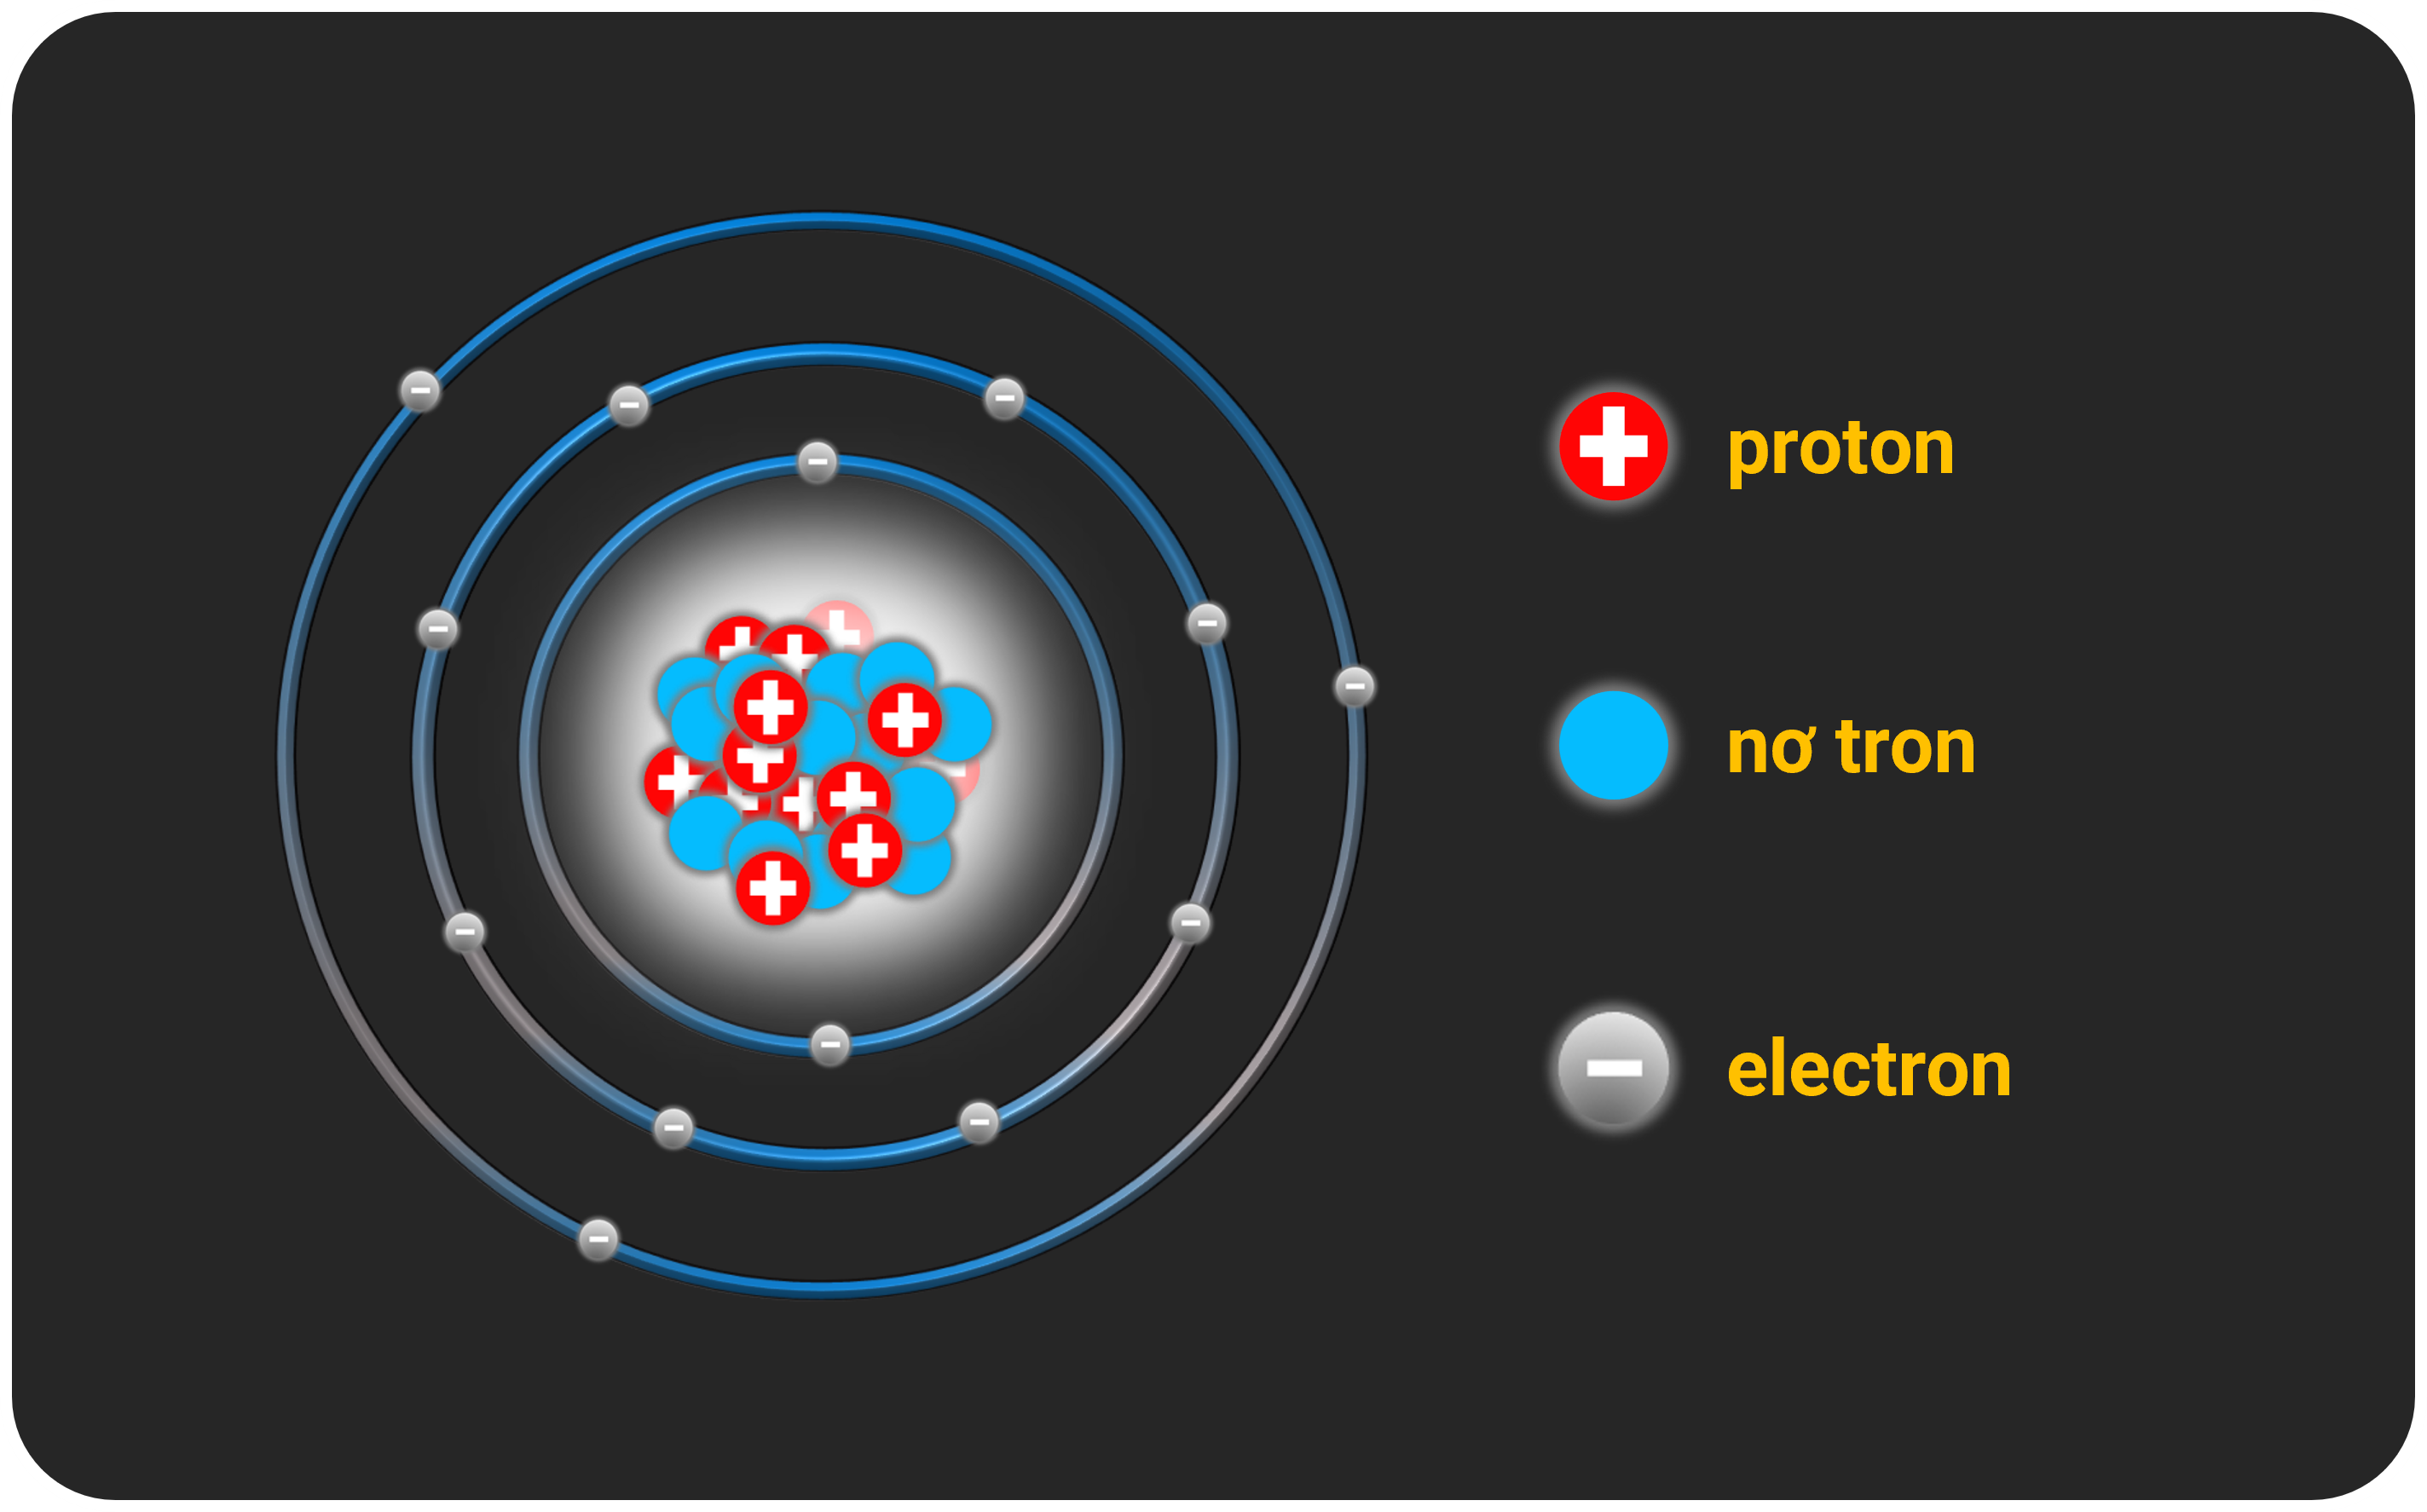
\includegraphics[width=5cm]{Images/anhhoahoc10/Mohinhnguyentu.png}
		\end{center}
		\loigiai{
			a) Hiện tượng nước phun vào bình cho thấy áp suất khí HCl trong bình đã giảm rất nhanh.
			\\
			Giải thích: Khi nhúng ống thủy tinh vào cốc nước, khí HCl hòa tan mạnh vào nước, làm giảm số lượng phân tử khí HCl trong bình. Do đó, áp suất trong bình giảm mạnh so với áp suất khí quyển bên ngoài, tạo ra sự chênh lệch áp suất khiến nước phun mạnh vào bình.
			\\
			b) Sự biến đổi áp suất như vậy đã chứng tỏ khí HCl tan rất tốt trong nước.
		}
	\end{bt}
\end{document}
